\documentclass[12pt,a4paper]{article}
\input{packages.tex}
\author{Mansilla, Kevin Gaston\footnote{\href{mailto:kevingston47@gmail.com}{kevingston47@gmail.com}}}
\title{Discreta II: Carpeta}
\date{\today}
\begin{document}
\maketitle{}

\tableofcontents

\section{Coloreo}
\underline{Algo de notación:}
\medskip

$d(x)$ es el grado de $x$, $\delta = \min \llaves{d(x):x\in V}$, $\Delta = \max \llaves{d(x):x\in V}$.
Si $\delta = \Delta$ es un grafo regular.

\subsection{Greedy}

\begin{teorema}(VIT) Sea $G$ un grafo que tiene un coloreo propio con $r$ colores. Y 
    sea $c_{1},c_{2},\ldots,c_{r}$ un ordenamiento de $r$ colores. Sea $V_{i} = \llaves{x\in V :\, color(x)=i}$
    ordenamos los vertices de $G$ tal que $V_{i}$ este antes de $V_{2}\ldots$ y corremos 
    greedy con ese orden. Entonces greedy colorea a $G$ con $\< r$ colores.
\end{teorema}
\underline{Demostración:} Se hace por inducción, cabe resaltar que greedy tiene 
complejidad $O(n)$.
\medskip

Sea el orden de coloreo: $w_{i} = V_{1} \cup V_{2} \cup \ldots \cup V_{i}$ con  $i=1,2,\ldots,r$.
\medskip

\underline{Hipotesis inductiva:} Greedy en ese orden, colorea $w_{i}$ con $\< i$ colores, si 
probamos HI como $w_{r} = V$ ya está.
\medskip

\underline{Caso Base:} $i=1$
\medskip

Tenemos que probar que Greedy colorea $V_{1}$ con $1$ color. Pero 
$V_{1} = \llaves{x \in G : \, color(x) = c_{1}}$ (con el que viene coloreado). 
Como $color(x)$ es un coloreo propio y todos los vertices de $V_{1}$ tienen el 
mismo color, no puede haber lados entre vertices de $V_{1}$. Entonces, Greedy los 
colorea a todos con un solo color.
\medskip

\underline{Paso Inductivo:} $i \rightarrow i+1$.
\medskip

Supongamos que \textbf{no vale} para $i+1$, es decir, que es falso que Greedy colorea $w_{i+1}$ 
con $\< i+1$ colores.
\medskip

Entonces \textbf{debe existir vertice $x \in w_{i+1}$ coloreado con color $i+2$} (si coloreamos 
con colores $1,2,\ldots,r+i$). Para que Greedy se vea forzado a colorear $x$ con 
$i+2$ debe existir un vecino de $x$ anterior a $x$ en el orden que estoy coloreando 
que tenga color $i+1$, llamemoslo $y$.
\medskip

Por HI, $w_{i}$ puede ser coloreado por Greedy con a lo sumo $i$ colores y como 
$i+1, i+2 > i$ entonces $x,y \notin w_{i}$. Pero $x \in w_{i+1}$ e $y$ es anterior 
a $x$ entonces $y \in w_{i+1}$. Entonces Tenemos:
$$x,y \in w_{i+1} = V_{1} \cup V_{2} \cup \ldots V_{i} \cup V_{i+1}$$
$$x,y \notin w{i} = V_{1} \cup V_{2} \cup \ldots V_{i}$$

Entonces si $x,y \in V_{i+1}$, por lo que $color(x)=color(y)=c_{i+1}$. Pero es un 
absurdo porque el coloreo original era propio y $x,y$ son vecinos.
$\square$

\begin{corolario} Existe un orden de los vértices tal que Greedy, en ese orden, 
    colorea $G$ con $\< \chi(G)$ colores.
\end{corolario}

\underline{Demostración:} 
\medskip

Sea $\chi(G) = min\llaves{k: \exists\, \text{coloreo propio de $G$ en $k$ colores}}$
\medskip

Entonces existe un coloreo propio de $G$ con $\chi(G)$ colores. Usamos el VIT 
ordenando los colores de alguna forma. Además por el VIT Greedy en ese orden colorea 
$G$ con $\chi(G)$ colores o menos.
\medskip

Es importante dar una una cota para $\chi(G)$. \underline{Prueba:}
\medskip

Cuando vamos a colorear un vertice $x$ con Greedy debemos mirar los colores de 
los vecinos anteriores a $x$ y no le podemos dar ninguno de esos colores. El peor 
caso posible es que todos los vecinos de $x$ sean vecinos anteriores y que todos 
tengan colores distintos.
\medskip

En el peor caso posible debo \textbf{eliminar} $d(x)$ colores con $d(x) = \Delta$ 
a lo sumo elimino $\Delta$ colores. Asi que si tengo $\Delta +1$ colores disponibles 
siempre habrá uno que sobre. Entonces $\chi(G) \< \Delta + 1$. 
\medskip

Los grafos completos alcanzan la cota $\Delta(K_{n}) = n-1 \rightarrow \chi(K_{n}) = n = \Delta +1$.
Y los grados impares $\Delta(C_{2r+1}) = 2 \rightarrow \chi(C_{2r+1}) = 3 = \Delta +1$.
$\square$

\begin{definition} Un camino en $G$ es una sucesión de vértices $x_{1},x_{2},\ldots,x_{r}$
    tales que $x_{i}x_{i+1} \in E$. $x \thicksim y \Longleftrightarrow \exists \,\text{camino entre $x$ e $y$}$
    (es una relación de equivalencia).
\end{definition}

\begin{teorema} (Broks) Sea $G$ un grado conexo que no sea un $K_{n}$ o $C_{2r+1}$. 
    Entonces $\chi(G) \< \Delta(G)$.
\end{teorema}

\underline{Demostración:} Para el caso no regular.
\medskip

Sea $x \in V$, tal que el grado $d(x) = \delta$. Corramos DFS o BFS a partir 
de $x$, como $G$ es conexo, encuentro todos los vertices, en el orden DFS o BFS.
\medskip

Vamos a correr Greedy en orden inverso. Por lo que si $x$ es el último vértice, 
en el orden DFS o BFS todo vertice es puesto por algún vecino que ya estaba. 
Entonces implica que todo vértice $(\neq x)$ tiene un vecino anterior en el orden 
BFS (o DFS) implica que en el orden inverso todo vertice $\neq x$ tiene un vecino 
posterior.
\medskip

Entonces cuando Greedy colorea un vértice $z$, debe mirar los vecinos anteriores 
$(z \neq x)$ como $z$ tiene un vecino posterior, los anteriores son $\< d(x) -1$.
\medskip

Entonces Greedy va a eliminar a los sumo $d(z) -1 \< \Delta -1$ colores. Entonces 
si tengo $\Delta$ colores, siempre va a sobrar uno para colorear a $z$ si $z \neq x$ 
y para colorear $x$ eliminamos a lo sumo $d(x) = \delta < \Delta$ colores. Por lo 
tanto lo puedo colorear. $\square$.
\medskip

\textbf{Problema:} "k-color": Dado $G$ es $\chi(G) \< k$? $1-$color es trivial 
(no es polinomial). $2-$color es polinoimal (hay algún algoritmo que corre en tiempo 
polinomial en un rango de la entrada). Idea (la demostración por ahora no) Basta 
correrlo para grados conexos. Tomamos un $x\in V$, corremos BFD empezando en $x$. Si:
\begin{align*}
    N(z) &=\, \text{nivel $z$ en el arbol BFS}\\
         &=\, \text{distancia entre $z$ y $x$ en el arbol BFS}\\
         &=\, \text{distancia entre $z$ y $x$ en $G$}
\end{align*}
Sea: 
\begin{align*}
    C(z) &= (N(z)\, mod\, 2)\\
    &IF(\text{$C$ es propio, return si, es $2-$colorable})\\
    &ELSE(\text{return no es $2-$colorable})
\end{align*}

El algoritmo es polinomial porque BFS es $O(m)$ y chequear que es propio es $O(m)$,
lo que hay que probar es si es correcto. Entonces supongamos que la respuesta es 
"no es $2-$colorable". 

$$\Rightarrow \exists v,x : c(v) = c(z) \wedge vz \in E$$

Entonces $d(x,v) = d(x,z)\,\,mod\,\, 2$
\medskip

tomamos un camino entre $x$ y $v$ en BFS y un camino entre $x$ y $z$ en BFS y sea 
$w$ el único vertice en común (como lo muestra la siguiente figura).

\begin{figure}[h!]
    \centering
    \tikzset{every picture/.style={line width=0.75pt}} %set default line width to 0.75pt        
    \begin{tikzpicture}[x=0.75pt,y=0.75pt,yscale=-1,xscale=1]
    %uncomment if require: \path (0,300); %set diagram left start at 0, and has height of 300
    \centering
    %Curve Lines [id:da9660361289294499] 
    \draw    (185,174) .. controls (254,182) and (276,96) .. (315,54) ;
    %Curve Lines [id:da45622019482482745] 
    \draw    (285,98) .. controls (325,68) and (330,217) .. (370,187) ;
    % Text Node
    \draw (312,31.8) node [anchor=north west][inner sep=0.75pt]    {$x$};
    % Text Node
    \draw (380,180.8) node [anchor=north west][inner sep=0.75pt]    {$z$};
    % Text Node
    \draw (172,170.8) node [anchor=north west][inner sep=0.75pt]    {$v$};
    % Text Node
    \draw (270,86.8) node [anchor=north west][inner sep=0.75pt]    {$w$};
    \end{tikzpicture}
\end{figure}

Miramos el ciclo en $G$: $w \ldots \underbrace{vz}_{\text{cruzo a $z$}} \ldots \underbrace{w}_{\text{vuelvo a $x$}}$ 
(como lo muestra la siguiente imagen).
\begin{figure}[h!]
    \centering
    \tikzset{every picture/.style={line width=0.75pt}} %set default line width to 0.75pt        
    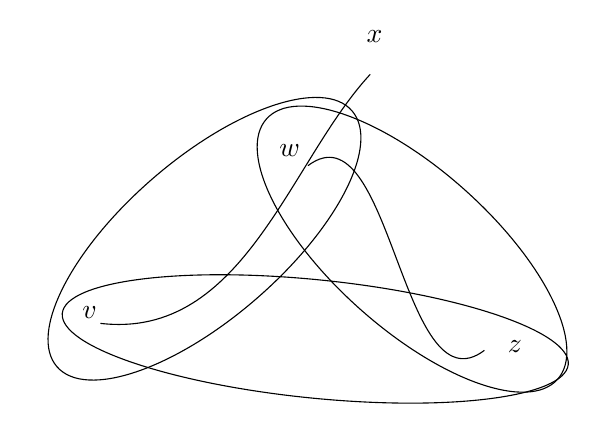
\begin{tikzpicture}[x=0.75pt,y=0.75pt,yscale=-1,xscale=1]
    %uncomment if require: \path (0,300); %set diagram left start at 0, and has height of 300
    %Curve Lines [id:da9660361289294499] 
    \draw    (185,174) .. controls (254,182) and (276,96) .. (315,54) ;
    %Curve Lines [id:da45622019482482745] 
    \draw    (285,98) .. controls (325,68) and (330,217) .. (370,187) ;
    %Shape: Ellipse [id:dp8919263115782621] 
    \draw   (164.05,194.88) .. controls (150.21,178.93) and (170.82,138.4) .. (210.07,104.35) .. controls (249.32,70.3) and (292.36,55.63) .. (306.19,71.58) .. controls (320.02,87.52) and (299.42,128.05) .. (260.17,162.1) .. controls (220.92,196.15) and (177.88,210.83) .. (164.05,194.88) -- cycle ;
    %Shape: Ellipse [id:dp6731791355972647] 
    \draw   (166.62,169.16) .. controls (168.21,153.5) and (224.06,146.33) .. (291.37,153.14) .. controls (358.68,159.96) and (411.96,178.18) .. (410.38,193.84) .. controls (408.79,209.5) and (352.94,216.67) .. (285.63,209.86) .. controls (218.32,203.04) and (165.04,184.82) .. (166.62,169.16) -- cycle ;
    %Shape: Ellipse [id:dp4061401367808297] 
    \draw   (265.02,75.48) .. controls (279.1,59.75) and (321.9,75.09) .. (360.61,109.74) .. controls (399.33,144.4) and (419.3,185.24) .. (405.22,200.97) .. controls (391.14,216.7) and (348.34,201.36) .. (309.63,166.71) .. controls (270.91,132.06) and (250.94,91.21) .. (265.02,75.48) -- cycle ;
    % Text Node
    \draw (312,31.8) node [anchor=north west][inner sep=0.75pt]    {$x$};
    % Text Node
    \draw (380,180.8) node [anchor=north west][inner sep=0.75pt]    {$z$};
    % Text Node
    \draw (175,164.8) node [anchor=north west][inner sep=0.75pt]    {$v$};
    % Text Node
    \draw (270,86.8) node [anchor=north west][inner sep=0.75pt]    {$w$};
    \end{tikzpicture}
\end{figure}

Calculamos la longitud de este ciclo:
\begin{align*}
    longitud &= 1 + d(v,w) + d(z,w) \\
    longitud\, mod\, 2 &= (1 + d(v,w) + \ldots + d(z,w)) \, mod\, 2\\
    &= (1 + d(v,w) + d(z,w) + 2d(x,w))\, mod\, 2\\
    &= (1 + d(x,v) + d(x,z))\, mod\, 2 = (1 + \overbrace{c(x) + c(z)}^{=0})\, mod\, 2\\
    &= 1
\end{align*}
Es un ciclo impar, entonces no se puede colorear con 2 colores $\Rightarrow$ $\chi_(G) \> 3$.
$\square$

\section{Flujos y networks:}

Un grafo dirigido es un par $(V,E)$ con $E \subseteq V \times V$. Un network (estructura) 
es un triple $(V,E,C)$ donde $(V,E)$ es un grafo dirigido y $C: E \to \mathbb{R}_{\>0}$ 
es la capacidad.
\medskip

Notación: Si $g$ está definida en $E$ y $A,B \subseteq V$ definimos:
$$g(A,V) = \sum_{x\in A,y\in B,xy \in E} g(x,y)$$

Dado $x \in V$, $g$ definida en $E$. Definimos:
\begin{align*}
    out_{g}(x) &= g(\llaves{x},V) = \sum_{y \in V, xy \in E} g(x,y)\\
    in_{g}(x) &= g(V,\llaves{x}) = \sum_{y \in V, yx \in E} g(y,x)\\
\end{align*}

Si $\overrightarrow{xy} = (x,y)$, entonces:
$$\Gamma^{+}(x) = \llaves{y : (x,y) \in E}$$

En cambio si $\overrightarrow{yx} = (y,x)$, tenemos:
$$\Gamma^{-}(x) = \llaves{y : (y,x) \in E} $$

Entonces, podemos definir:
\begin{align*}
    out_{g}(x) &= \sum_{y \in \Gamma^{+}(x)} g(\overrightarrow{xy})\\
    in_{g}(x) &= \sum_{y \in \Gamma^{-}(x)} g(\overrightarrow{yx})\\
\end{align*}
Dado un network $(V,E,C)$ y vertices $s,t$ un flujo de $s$ a $t$ es una función 
$f$ en los lados con ($s$ es la fuente y $t$ el sumidero):
\begin{itemize}
    \item [a)] $0 \< f(\overrightarrow{xy}) \< c(\overrightarrow{xy})$ para todo $\overrightarrow{xy} \in E$.
    \item [b)] $In_{f}=Out_{f}, \,\forall x \neq s,t$ (la red no tiene perdidas en los vertices de transito).
    \item [c)] $In_{f}(s) = Out_{f}(t) = 0$ 
\end{itemize}

El valor del flujo es $v(f) = out_{f}(s) - in_{f}(s) = out_{f}(s)$. Un flujo es 
máximal si $v(g) \< v(f), \, \forall g$ flujo de $s$ a $t$. Entonces, el problema 
de maxflow, dado un network hallar flujo maximal.
\medskip

\underline{Propiedad:} $V(f) = In_{f}(t)$
\begin{align*}
    f(V,V) = \sum_{x,y \in V, x,y\in E} f(\overrightarrow{xy}) &= \sum_{x\in V} \parent{\sum_{y\in V, \overrightarrow{xy}\in E}f(\overrightarrow{xy})}\\
    &= \sum_{x \in V} out_{f}(x)
\end{align*}
Por otro lado,
\begin{align*}
    f(V,V) = \sum_{z \in V, \overrightarrow{zx}\in E} f(\overrightarrow{zx}) &= \sum_{x\in V} \parent{\sum_{z\in V, \overrightarrow{zx}\in E} f(\overrightarrow{zx})}\\
    &= \sum_{x\in V} In_{f}(x)\\
\end{align*}
Entonces
\begin{align*}
    &\sum In_{f}(x) = \sum out_{f}(x)\\
    &\sum_{x\in V}\parent{In_{f}(x) - out_{f}(x)} = 0,\, \text{si $x=s,t$}\\
    &=\llaves{\text{Como en $s$ no entra flujo y en $t$ no sale}}\\
    \Rightarrow &\underbrace{In_{f}(s)}_{=0} - out_{f}(s) + In_{f}(t) - \underbrace{out_{f}(t)}_{=0} = 0\\
    \Rightarrow &- out_{f}(s) + in_{f}(t) = 0\\
    &out_{f}(s) - In_{f}(t) = v(f) \geq 0\\
    &\square
\end{align*} 

\begin{definition} Un camino dirigido desde $x$ a $y$ es una sucesión de vértices 
    $x_{0}, x_{1}, \ldots, x_{r}$ con $x_{0} = x, x_{r} = y$. Pues $\overrightarrow{x_{i}x_{i+1}}\in E$.
\end{definition}

\subsection{Algoritmo Greedy aplicado a networks:}
\begin{align*}
    &\text{Empezar con flujo $f = 0$}\\
    &\text{Mientras se pueda, hacer lo siguiente}\\
    &\,\,\,\,\,\,\text{Hallar camino dirigido desde $s$ a $t$ tal que $f(\overrightarrow{x_{i}x_{i+1}}) < c(\overrightarrow{x_{i}x_{i+1}})$}\\
    &\,\,\,\,\,\,\text{Tomar $e = min \llaves{c(\overrightarrow{x_{i}x_{i+1}}) - f(\overrightarrow{x_{i}x_{i+1}}) : \overrightarrow{x_{i}x_{i+1}} \in E}$}\\
    &\,\,\,\,\,\,\text{Tomar $f^{*}$ tal que:} \\
    &\,\,\,\,\,\,f^{*}(\overrightarrow{xy})= \left\{ \begin{array}{lcc}
            f(\overrightarrow{xy}) & si & xy \neq \overrightarrow{x_{i}x_{i+1}}\, \forall i \\
            \\ f(\overrightarrow{x_{i}x_{i+1}}) + e& si & \overrightarrow{xy} = \overrightarrow{x_{i}x_{i+1}}\\
            \end{array}
            \right.\\
    &\,\,\,\,\,\,\text{Hacer $f=f^{*}$}\\
\end{align*}

\subsection{FF (Greedy alterado)}
Es alterado porque ahora se puede devolver flujo además de mandar.
\medskip

\begin{definition} Dado un flujo $f$ en un network un camino aumentante (o $f-$camino aumentante)
    es una sucesión de vertices $x_{0},x_{1},\ldots x_{r}$ tal que $x_{0}=s$ y $x_{r}=t$ y tal que 
    $\forall t < r$ pasa una de las siguientes dos cosas:
    \begin{itemize}
        \item [1.] $\overrightarrow{x_{i}x_{i+1}} \in E \land f(\overrightarrow{x_{i}x_{i+1}}) < c(\overrightarrow{x_{i}x_{i+1}})$
            (puedo mandar más flujo por ese lado - lado fordward).
        \item [2.] $\overrightarrow{x_{i+1}x_{i}} \in E \land f(\overrightarrow{x_{i+1}x_{i}}) > 0$ 
            (importa que haya mandado flujo - lado backward).
    \end{itemize}
\end{definition}

\underline{Algoritmo de Ford-Fulkerson (Greedy con camino aumentante):}
\begin{itemize}
    \item [1.] $f = 0$
    \item [2.] Buscar un camino aumentante $s=x_{0},x_{1},\ldots,x_{r}=t$.
    \item [3.] Defino:
        $$\epsilon_{i}= \left\{ \begin{array}{lcc}
        c(\overrightarrow{x_{i}x_{i+1}}) - f(\overrightarrow{x_{i}x_{i+1}}) & \text{en los lados fordward} \\
        \\ f(\overrightarrow{x_{i+1}x_{i}})& \text{no puedo devolver más de lo que me mandan}\\
        \end{array}
        \right.$$
        $\epsilon = min\llaves{\epsilon_{i}}$
    \item [4.] Cambiar $f$ a lo largo del camino.
        \begin{align*}
            f(\overrightarrow{x_{i}x_{i+1}}) &= f(\overrightarrow{x_{i}x_{i+1}}) + \epsilon\,\, \text{en fordward}\\
            f(\overrightarrow{x_{i+1}x_{i}}) &= f(\overrightarrow{x_{i+1}x_{i}}) - \epsilon\,\, \text{en backward}
        \end{align*}
        y repetir 2 hasta que se pueda.
    \item [5.]
        return $f$.
\end{itemize}

\underline{Correctitud de F-F:}
\begin{definition} Un corte es un $S \subseteq V$ tal que $s \in S, t \notin S$.
\end{definition}

Ejemplo:
\begin{align*}
    S_{1} = \llaves{s}\\
    S_{2} = V - \llaves{t}\\
\end{align*}

Son los cortes triviales, cabe resaltar que puede haber a lo sumo hay $2^{n-2}$ cortes.
\medskip

La capacidad de un corte es:
\begin{align*}
    cap(S) &= c(S,\overline{S} ) \\
    &= \sum_{x \in S, y\notin S, \overrightarrow{xy}\in E} c(\overrightarrow{xy})\\
\end{align*}
Un corte $S$ es minimal si $cap(S) = cap(T), \forall T$ corte.

\begin{lema} Al cambiar el flujo $f$ como en el algoritmo de F-F a un $f^{*}$, lo 
    que queda es flujo y $v(f^{*}) = v(f) + \epsilon$
\end{lema}
\underline{Demostración:}
\medskip

Lados fordward:
\begin{align*}
    f^{*}(\overrightarrow{x_{i}x_{i+1}}) &= f(\overrightarrow{x_{i}x_{i+1}}) + \epsilon \< c(\overrightarrow{x_{i}x_{i+1}})\\
    & \text{con}\, \epsilon \in \epsilon_{i} = c(\overrightarrow{x_{i}x_{i+1}}) - f(\overrightarrow{x_{i}x_{i+1}})\\
\end{align*}

Lados backward:
\begin{align*}
    &f^{*}(\overrightarrow{x_{i+1}x_{i}}) = f(\overrightarrow{x_{i+1}x_{i}}) - \epsilon \> 0\\
    &\epsilon \in \epsilon_{i} = f(\overrightarrow{x_{i+1}x_{i}})\\
\end{align*}

\textbf{Tenemos que ver que} $in_{f}(x) = out_{f}(x), \forall x \neq s,t$.
\medskip

Si $x \neq x_{i}$ entonces: 
\begin{align*}
    &in_{f^{*}}(x) = in_{f}(x)\\
    &out_{f^{*}}(x) = out_{f}(x)\\
    &\Rightarrow in_{f^{*}}(x) = out_{f^{*}}(x)
\end{align*}

Supongamos ahora que $x = x_{i}, x=s,t \Rightarrow \exists x_{i-1},x_{i+1}$. Tenemos lo siguientes casos:
\medskip

\underline{Caso 1:} $x_{i-1}x_{i}, x_{i}x_{i+1}$ fordwards. Como lo muestra la siguiente imagen:
\begin{figure}[h!]
    \centering
    \tikzset{every picture/.style={line width=0.75pt}} %set default line width to 0.75pt        

    \begin{tikzpicture}[x=0.75pt,y=0.75pt,yscale=-1,xscale=1]
    %uncomment if require: \path (0,300); %set diagram left start at 0, and has height of 300

    %Curve Lines [id:da05255710943316538] 
    \draw    (205,177) .. controls (212,107) and (326,83) .. (374,92) ;

    % Text Node
    \draw (188,182.8) node [anchor=north west][inner sep=0.75pt]    {$x_{i-1}$};
    % Text Node
    \draw (246,88.8) node [anchor=north west][inner sep=0.75pt]    {$x$};
    % Text Node
    \draw (376,86.8) node [anchor=north west][inner sep=0.75pt]    {$x_{i+1}$};
    \end{tikzpicture}
\end{figure}

Si mandamos $\epsilon$ de $x_{i-1}$ a $x_{i}$ y de $x_{i}$ a $x_{i+1}$ entonces:
\begin{figure}[h!]
    \centering
    \tikzset{every picture/.style={line width=0.75pt}} %set default line width to 0.75pt        
    \begin{tikzpicture}[x=0.75pt,y=0.75pt,yscale=-1,xscale=1]
    %uncomment if require: \path (0,300); %set diagram left start at 0, and has height of 300
    %Curve Lines [id:da05255710943316538] 
    \draw    (205,177) .. controls (212,107) and (326,83) .. (374,92) ;
    \draw   (199.97,154.97) .. controls (207.02,153.34) and (212.47,150.6) .. (216.35,146.75) .. controls (214.07,151.71) and (213.38,157.78) .. (214.28,164.95) ;
    \draw   (286.9,93.5) .. controls (293.74,95.85) and (299.82,96.4) .. (305.15,95.19) .. controls (300.58,98.19) and (296.79,102.97) .. (293.76,109.54) ;
    % Text Node
    \draw (188,182.8) node [anchor=north west][inner sep=0.75pt]    {$x_{i-1}$};
    % Text Node
    \draw (249,95.8) node [anchor=north west][inner sep=0.75pt]    {$x$};
    % Text Node
    \draw (376,86.8) node [anchor=north west][inner sep=0.75pt]    {$x_{i+1}$};
    % Text Node
    \draw (203,120.8) node [anchor=north west][inner sep=0.75pt]    {$+\epsilon $};
    % Text Node
    \draw (299,74.8) node [anchor=north west][inner sep=0.75pt]    {$+\epsilon $};
    \end{tikzpicture}
\end{figure}

Entonces tenemos:
\begin{align*}
    in_{f^{*}}(x_{i}) &= in_{f}(x) + \epsilon\\
    out_{f^{*}}(x_{i}) &= out_{f}(x) + \epsilon\\
    \Rightarrow in_{f^{*}}(x_{i}) &= out_{f^{*}}(x_{i})
\end{align*}

\underline{Caso II:} Ambos lados backwards
\begin{figure}[h!]
    \centering
    \tikzset{every picture/.style={line width=0.75pt}} %set default line width to 0.75pt        
    \begin{tikzpicture}[x=0.75pt,y=0.75pt,yscale=-1,xscale=1]
    %uncomment if require: \path (0,300); %set diagram left start at 0, and has height of 300
    %Curve Lines [id:da05255710943316538] 
    \draw    (205,177) .. controls (212,107) and (326,83) .. (374,92) ;
    \draw   (229.21,142.29) .. controls (222.42,144.78) and (217.35,148.18) .. (213.98,152.48) .. controls (215.63,147.28) and (215.56,141.17) .. (213.77,134.16) ;
    \draw   (308.39,103.62) .. controls (301.64,101.01) and (295.58,100.22) .. (290.21,101.24) .. controls (294.89,98.41) and (298.86,93.77) .. (302.14,87.32) ;
    % Text Node
    \draw (188,182.8) node [anchor=north west][inner sep=0.75pt]    {$x_{i-1}$};
    % Text Node
    \draw (249,95.8) node [anchor=north west][inner sep=0.75pt]    {$x$};
    % Text Node
    \draw (376,86.8) node [anchor=north west][inner sep=0.75pt]    {$x_{i+1}$};
    % Text Node
    \draw (201,111.8) node [anchor=north west][inner sep=0.75pt]    {$-\epsilon $};
    % Text Node
    \draw (299,74.8) node [anchor=north west][inner sep=0.75pt]    {$-\epsilon $};
    \end{tikzpicture}
\end{figure}

Entonces:
\begin{align*}
    out_{f^{*}}(x_{i}) &= out_{f}(x_{i}) - \epsilon\\
    in_{f^{*}}(x_{i}) &= in_{f}(x_{i}) - \epsilon\\
    \Rightarrow in_{f^{*}}(x_{i}) &= out_{f^{*}}(x_{i})
\end{align*}

\underline{Caso III:}
\begin{figure}[h!]
    \centering
    \tikzset{every picture/.style={line width=0.75pt}} %set default line width to 0.75pt        
    \begin{tikzpicture}[x=0.75pt,y=0.75pt,yscale=-1,xscale=1]
    %uncomment if require: \path (0,300); %set diagram left start at 0, and has height of 300
    %Curve Lines [id:da05255710943316538] 
    \draw    (205,177) .. controls (212,107) and (326,83) .. (374,92) ;
    \draw   (203.03,150.33) .. controls (210.03,148.49) and (215.39,145.58) .. (219.15,141.61) .. controls (217.01,146.64) and (216.51,152.72) .. (217.64,159.87) ;
    \draw   (308.39,103.62) .. controls (301.64,101.01) and (295.58,100.22) .. (290.21,101.24) .. controls (294.89,98.41) and (298.86,93.77) .. (302.14,87.32) ;
    % Text Node
    \draw (188,182.8) node [anchor=north west][inner sep=0.75pt]    {$x_{i-1}$};
    % Text Node
    \draw (249,95.8) node [anchor=north west][inner sep=0.75pt]    {$x$};
    % Text Node
    \draw (376,86.8) node [anchor=north west][inner sep=0.75pt]    {$x_{i+1}$};
    % Text Node
    \draw (197,117.8) node [anchor=north west][inner sep=0.75pt]    {$+\epsilon $};
    % Text Node
    \draw (299,74.8) node [anchor=north west][inner sep=0.75pt]    {$-\epsilon $};
    \end{tikzpicture}
\end{figure}

Entonces:
\begin{align*}
    out_{f^{*}}(x_{i}) &= out_{f}(x_{i})\\
    in_{f^{*}}(x_{i}) &= in_{f}(x_{i}) - \epsilon + \epsilon\\
    \Rightarrow in_{f^{*}}(x_{i}) &= out_{f^{*}}(x_{i})
\end{align*}

\underline{Caso IV:}
\begin{figure}[h!]
    \centering
    \tikzset{every picture/.style={line width=0.75pt}} %set default line width to 0.75pt        
    \begin{tikzpicture}[x=0.75pt,y=0.75pt,yscale=-1,xscale=1]
    %uncomment if require: \path (0,300); %set diagram left start at 0, and has height of 300
    %Curve Lines [id:da05255710943316538] 
    \draw    (205,177) .. controls (212,107) and (326,83) .. (374,92) ;
    \draw   (229.21,142.29) .. controls (222.42,144.78) and (217.35,148.18) .. (213.98,152.48) .. controls (215.63,147.28) and (215.56,141.17) .. (213.77,134.16) ;
    \draw   (286.44,94.68) .. controls (293.5,96.29) and (299.6,96.19) .. (304.77,94.41) .. controls (300.55,97.89) and (297.29,103.05) .. (294.98,109.91) ;
    % Text Node
    \draw (188,182.8) node [anchor=north west][inner sep=0.75pt]    {$x_{i-1}$};
    % Text Node
    \draw (249,95.8) node [anchor=north west][inner sep=0.75pt]    {$x$};
    % Text Node
    \draw (376,86.8) node [anchor=north west][inner sep=0.75pt]    {$x_{i+1}$};
    % Text Node
    \draw (201,111.8) node [anchor=north west][inner sep=0.75pt]    {$-\epsilon $};
    % Text Node
    \draw (299,74.8) node [anchor=north west][inner sep=0.75pt]    {$+ \epsilon $};
    \end{tikzpicture}
\end{figure}

Entonces:
\begin{align*}
    in_{f^{*}}(x_{i}) &= in_{f}(x_{i})\\
    out_{f^{*}}(x_{i}) &= out_{f}(x_{i}) - \epsilon + \epsilon\\
    \Rightarrow in_{f^{*}}(x_{i}) &= out_{f^{*}}(x_{i})
\end{align*}

Por lo que:
\begin{align*}
    v(f^{*}) &= out_{f^{*}}(S) \\
    &= out_{f}(S) + \epsilon\\
    &= v_{f}(S) + \epsilon
\end{align*}

\subsection{Max-flow-min-cut theorem}
\begin{teorema} 
    \begin{itemize}
        \item [a.] $f$ flujo, $S$ corte $\Rightarrow v(f) = f(S,\overline{S}) - f(\overline{S},S)$
        \item [b.] $f$ flujo, $S$ corte $\Rightarrow v(f) \< cap(S)$
        \item [c.] Si $f$ es flujo las siguientes son equivalentes:
            \begin{itemize}
                \item [1.] $\exists S$ corte: $v(f) = cap(S)$
                \item [2.] $f$ es maximal.\\
                $(1=2)$ dice: \\
                "$f$ maximal $\Longleftrightarrow \exists S$ corte $v(f) = cap(S)$"\\
                y se suele llamar 'max-flow-min-cut theorem'.
                \item [3.] $\nexists f-$caminos aumentanes entre $s$ y $t$ 
            \end{itemize}
    \end{itemize}
\end{teorema}

\underline{Demostración:}
\medskip

\begin{itemize}
    \item [a.] $f$ flujo, $S$ corte $\Rightarrow v(f) = f(S,\overline{S}) - f(\overline{S},S)$
\end{itemize}

\underline{Prueba:}
\medskip

Sea $A = \sum_{x\in S} \corchet{out_{f}(x) - in_{f}(x)}$, como $out_{f}(x) = in_{f}(x), \forall x \in s,t$. 
Si tenemos que $s \in S$ (todos ceros menos el correspondiente al $S$) y $t \notin S$, entonces:
\begin{align*}
    A &= out_{f}(S) - \overbrace{in_{f}(S)}^{=0} + 0 + 0\\
    A &= v(f)
\end{align*}

Por otro lado:
\begin{align*}
    A = \sum_{x\in S} \corchet{out_{f}(x) - in_{f}(x)} &= \sum_{x\in S} out_{f}(x) - \sum_{x\in S} in_{f}(x)\\
    &= \sum_{x\in S} \overbrace{f(\llaves{x},V)}^{\text{todo lo que sale}} - \sum_{x\in S} \overbrace{f(V,\llaves{x})}^{\text{todo lo que entra}}\\
    &\text{por definición:}\\
    &= f(S,V) - f(V,S)\\
    &= f(S,S \cup \overline{S}) - f(S \cup \overline{S},S)\\
    &= \cancel{f(S,S)} + f(S,\overline{S}) \cancel{- f(S,S)} - f(\overline{S},S)\\
    &= f(S,\overline{S}) - f(\overline{S},S)
\end{align*}

\begin{itemize}
    \item [b.] $f$ flujo, $S$ corte $\Rightarrow v(f) \< cap(S)$
\end{itemize}
\underline{Prueba:}

Sale directo de $a)$:
\begin{align*}
    v(f) &= f(S,\overline{S}) \underbrace{- \underbrace{f(\overline{S},S)}_{\> 0}}_{\<0}\\
    &\< f(S,\overline{S}) \< \underbrace{c(S,\overline{S})}_{0\< f \< c} = cap(S)\\
\end{align*}

\begin{itemize}
    \item [c.] Si $f$ es flujo las siguientes son equivalentes:
    \begin{itemize}
        \item [1.] $\exists S$ corte: $v(f) = cap(S)$
        \item [2.] $f$ es maximal.\\
        $(1=2)$ dice: \\
        "$f$ maximal $\Longleftrightarrow \exists S$ corte $v(f) = cap(S)$"\\
        y se suele llamar 'max-flow-min-cut theorem'.
        \item [3.] $\nexists f-$caminos aumentanes entre $s$ y $t$\\
        y si se cumplen, el $s$ es minimal.
    \end{itemize}
\end{itemize}

\underline{Prueba} $1) \Rightarrow 2) \Rightarrow 3) \Rightarrow 1)$.
\medskip

$1) \Rightarrow 2)$ Sea $g$ un flujo por la parte b, del teorema:
$$v(g) \< cap(S) = v(f) \Rightarrow v(g) \< v(f) \Rightarrow f\, \text{maximal}$$

Además $S$ es minimal pues $T$ corte:
$$\Rightarrow cap(T) \> v(f) = cap(S) \Rightarrow S\, \text{minimal}$$

$2) \Rightarrow 3)$ Supongamos $f$ maximal y que es falso, $\lnot\, 3) \Rightarrow \lnot\, 2)$ (contrareciproca)
\medskip

Entonces, existe un $f-$camino aumentante entre $s$ y $t$, entonces usando ese camino aumentante 
podemos construir un nuevo flujo con valor $f^{*}$ tal que $v(f^{*}) = v(f) + \epsilon$ 
esto implica que $f$ no es maximal.
\medskip

$3) \Rightarrow 1)$, la idea es $\nexists \Rightarrow \exists$ (parte dificil)
\medskip

Definamos:
$$S = \llaves{s} \cup \llaves{x: \exists \, \text{un $f$ ca entre $s$ y $x$}}$$

Como $f$ es flujo y $S$ es corte, por la parte a:
$$v(f) = f(S,\overline{S}) - f(\overline{S},S)$$

Entonces:
$$f(S,\overline{S}) = \sum_{x\in S, y\in \overline{S}, xy \in E} f(\overrightarrow{xy})$$

Y tomemos un par $(x,y)$ cualquiera con $x\in S, y \notin S, xy \in E$, entonces 
existe un $f-$camino aumentante entre $s\ldots x$ y como $y \notin S$ no existe $f-$ca entre $s\ldots y$.
\medskip

Supongamos que $f(\overrightarrow{xy}) < c(\overrightarrow{xy})$, no se satura, 
entonces el lado $\overrightarrow{xy}$ puede usarse en algún ca. Como $s\ldots x$ 
es $f-$ca, entonces $s\ldots xy$ es $f-$ca, entonces $y \in S$, lo que es un absurdo.
\medskip

Conclusión: $f(\overrightarrow{xy}) \nless c(\overrightarrow{xy}) \Rightarrow f(\overrightarrow{xy}) = c(\overrightarrow{xy})$ 
esto vale $\forall x\in S, y\notin S, \overrightarrow{xy}\in E$. Por lo tanto:
$$f(S,\overline{S}) = \sum_{x\in S, y\notin S, xy \in E} f(\overrightarrow{xy}) = \sum_{x\in S, y\notin S}c(\overrightarrow{xy}) = c(S,\overline{S}) = cap(\overline{S})$$

Por otro lado, si es un lado backward:
$$f(\overline{S},S) = \sum_{x\notin S, y\in S, xy \in E} f(\overrightarrow{xy})$$

tomemos un par $(x,y)$ cualquiera con $\overrightarrow{xy} \in E, x\notin S, y\in S$, 
entonces $\exists f-$ca, $s\ldots y$
\medskip

Supongamos que $f(\overrightarrow{xy}) > 0$, entonces podemos devolver flujo por 
$\overrightarrow{xy}$ por lo que:
$$\underbrace{s\ldots y}_{ca}\overleftarrow{x}$$ 

también es ca, entonces $x\in S$ lo que es un absurdo, entonces $f(\overrightarrow{xy}) = 0, \forall x\notin S, y\in S, \overrightarrow{xy}\in E$
\medskip

Entonces:
$$f(\overline{S},S) = \sum_{x\notin S, y\in S, xy\in E} f(\overrightarrow{xy}) = 0$$

Por lo tanto:
$$v(f) = f(S,\overline{S}) - f(\overline{S},S) = cap(S) - 0 = cap(S)$$
$$\square$$


\begin{corolario} Si F-F termina, termina con flujo minimal
\end{corolario}

\underline{Complejidad de F-F:} Primero veamos.
\medskip

\underline{Complejidad de Greedy con camino aumentante solo con lados fwd:}
\begin{itemize}
    \item [1.] Buscamos camino dirigido $\to O(m)$.
    \item [2.] Cada camino que se usa, satura al menos un lado.
    \item [3.] Por 2, hay $O(m)$ caminos. $\Rightarrow O(m^{2})$.
\end{itemize}

\underline{F-F:}
\begin{itemize}
    \item [1.] Buscamos camino dirigido $\to O(m)$.
    \item [2.] Cada camino que se usa, satura o vacia al menos un lado.
    \item [3.] \textbf{No vale en greedy porque no devuelvo flujo.}\\
        Como en F-F un lado puede desaturarse y luego volver a saturarse o vaciarse 
        o luego llenarse, entonces $2) \Rightarrow 3)$ en F-F. Entonces, la complejidad 
        es $\infty$ porque puede no terminar. Hay que buscar caminos de longitud 
        minima, en ese caso si términa.
\end{itemize}

\subsection{Teorema de integralidad}
\begin{teorema} (Integralidad) Si las capacidades son enteras F-F termina y el 
    flujo maximal que se obtiene es entero.
\end{teorema}

\underline{Demostración:}
\medskip

Si $f$ es entero, entonces:
$$\epsilon_{i}= \left\{ \begin{array}{lcc}
    c(\overrightarrow{x_{i}x_{i+1}}) - f(\overrightarrow{x_{i}x_{i+1}}) & \to & \text{entero} \\
    \\ f(\overrightarrow{x_{i+1}x_{i}})& \to & \text{entero}\\
    \end{array}
    \right.$$

los $\epsilon_{i}$ serán enteros entonces $\epsilon$ sera entero, entonces:
$$f= \left\{ \begin{array}{lcc}
    f+\epsilon & \to & \text{entero} \\
    \\ f-\epsilon& \to & \text{entero}\\
    \end{array}
    \right.$$

seguira siendo entero. Además como empezamos con $f=0$ (entero), entonces $f$ entero 
es un invariante, que al terminar nos dice que $f$ será entero y termina porque:
$$v(f_{nuevo}) = v(f_{viejo}) + \epsilon \> v(f_{viejo}) + 1$$

Alguna vez termina pues $v(f) \< cap(\llaves{s})$

\subsection{Complejidad EK}
\begin{teorema} La complejidad de EK es $O(m^{2}n)$
    \label{teo:ek}
\end{teorema}

\begin{corolario} Siempre existen flujos maximales (siempre termina y termina con 
    un flujo maximal).
\end{corolario}
\underline{Prueba:}
\medskip

Dados $x,z$ vértices y $f$ flujo, definimos:
\begin{align*}
    d_{f}(x,z) &= \text{menor longitud de un $f-$ca entre $x$ y $z$}\\
    &=0\,, \text{si $x=z$}\\
    &=\infty\,, \text{si no existe $f-$ca entre $x$ y $z$}
\end{align*}

Sean $f_{0},f_{1},f_{2},f_{3},\ldots$ los flujos producidos por EK. Denotamos para 
un flujo $k$.
\begin{align*}
    d_{k}(x) = d_{f_{k}}(s,x)\\
    b_{k}(x) = d_{f_{k}}(x,t)
\end{align*}

que representan lo siguiente:
\begin{figure}[h!]
    \centering
    \tikzset{every picture/.style={line width=0.75pt}} %set default line width to 0.75pt        
    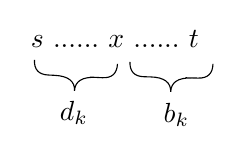
\begin{tikzpicture}[x=0.75pt,y=0.75pt,yscale=-1,xscale=1]
    %uncomment if require: \path (0,300); %set diagram left start at 0, and has height of 300
    %Shape: Brace [id:dp738535768547266] 
    \draw   (101,123) .. controls (100.77,127.66) and (102.98,130.11) .. (107.64,130.34) -- (110.66,130.49) .. controls (117.32,130.82) and (120.53,133.32) .. (120.3,137.98) .. controls (120.53,133.32) and (123.98,131.16) .. (130.64,131.49)(127.64,131.34) -- (133.66,131.64) .. controls (138.32,131.87) and (140.77,129.66) .. (141,125) ;
    %Shape: Brace [id:dp2855958534702414] 
    \draw   (147,124) .. controls (146.89,128.67) and (149.16,131.06) .. (153.82,131.17) -- (156.83,131.25) .. controls (163.5,131.42) and (166.77,133.83) .. (166.65,138.49) .. controls (166.77,133.83) and (170.16,131.58) .. (176.82,131.75)(173.82,131.67) -- (179.83,131.82) .. controls (184.5,131.94) and (186.89,129.67) .. (187,125) ;
    % Text Node
    \draw (98,107.8) node [anchor=north west][inner sep=0.75pt]    {$s\ ......\ x\ ......\ t$};
    % Text Node
    \draw (112,141.8) node [anchor=north west][inner sep=0.75pt]    {$d_{k}$};
    % Text Node
    \draw (162,142.8) node [anchor=north west][inner sep=0.75pt]    {$b_{k}$};
    \end{tikzpicture}
\end{figure}

Vamos a demostrar que $d_{k} \< d_{k+1}$, $b_{k} \< b_{k+1}$ (las distancias no 
disminuyen, la demostración para $b_{k} \< b_{k+1}$ es análoga)
\medskip

Sea $A = \llaves{y: d_{k+1}(y) < d_{k}(y)}$. Queremos ver que $A = \emptyset$ vamos 
a suponer que no es $\emptyset$ y llegar a un absurdo.
\medskip

Suponemos $A \neq \emptyset$, es decir, que tiene $1$ o muchos elementos, y de 
entre todos los elementos elegimos $x \in A$ tal que:
\begin{equation}
    d_{k+1}(x) \< d_{k+1}(y)\,\, \forall y \in A
    \label{EK:1}
\end{equation}

Como $x \in A$, entonces $d_{k+1}(x) < d_{k}(x) \Rightarrow d_{k+1} < \infty$, por 
definición de $A$.
Entonces, existe $f_{k+1}-$ca entre $s$ y $x$, tomemos uno de menor longitud, es decir,
\begin{align*}
    \underbrace{s .... x}_{longitud = d_{k+1}(x)}\\
\end{align*}

\underline{Observación:} $d_{k}(s) = d_{k+1}(s) = 0, s\notin A \ldots s \neq x$.
\medskip

Sea $z$ el vertice inmediatamente anterior a $x$ en ese camino $(s\ldots zx)$. 
Como el camino es de \textbf{longitud minima}, entonces:
\begin{equation}
    d_{k+1}(x) = d_{k+1}(z) + 1
    \label{EK:2}
\end{equation}

En particular, $d_{k+1}(z) < d_{k+1}(x) \Rightarrow_{Por \eqref{EK:1}} z \notin A$. 
(tendría que ser $\leq$)
\medskip

Como $z \notin A$, entonces se da lo contrario:
\begin{equation}
    d_{k}(z) \< d_{k+1}(z) \Rightarrow d_{k}(z) < \infty
    \label{EK:3}
\end{equation}

Como $d_{k+1}(z) < d_{k+1}(x) < \infty$. Por \eqref{EK:3} existe un $f_{k}-$ca 
entre $s$ y $z$, y de ellos voy a tomar uno de longitud minima.
\medskip

Pero primero supongamos que $\overrightarrow{zx} \in E$. Es $f_{k}(\overrightarrow{zx}) = c(\overrightarrow{zx})$ o no?.
Entonces, si suponemos primero que esta saturado $(f_{k}(\overrightarrow{zx}) = c(\overrightarrow{zx})$, 
pero $\underbrace{s\ldots z}_{f_{k+1}}x$ es un ca relativo. Entonces, $f_{k+1}(\overrightarrow{zx}) < c(\overrightarrow{zx})$.
Esto implica que para pasar de $f_{k}$ a $f_{k+1}$ el lado se uso backward.
\medskip

Entonces, para pasar de $f_{k}$ a $f_{k+1}$ debe haber un ca de la forma 
$s \ldots \overleftarrow{xz} \ldots t$ y como estamos usando EK este camino es de 
longitud minima.
\begin{equation}
    d_{k}(z) = d_{k}(x) + 1
    \label{EK:4}
\end{equation}

Entonces:
\begin{align*}
    d_{k}(x) =_{\eqref{EK:4}} d_{k}(z)-1 \< _{\eqref{EK:3}} d_{k+1}(z) -1 = (d_{k+1}(x)-1)-1 &= d_{k+1}(x) -2\\
    &<d_{k}(x) -2\\
    &\Rightarrow d_{k}(x) < d_{k+1}(x)-2 \\
    &\Rightarrow 0 < 2 \,\,\text{Absurdo}
\end{align*}

Llegamos a un absurdo por suponer que $f_{k}(\overrightarrow{zx}) = c(\overrightarrow{zx})$. 
Ahora veamos el otro caso, $f_{k}(\overrightarrow{zx}) < c(\overrightarrow{zx})$ (no esta saturado).
Pero teniamos el $f-k$ ca, $s \ldots z$ entonces existe un $f-k$ ca del tipo $s\ldots zx$.
\medskip

Entonces: 
\begin{align*}
    d_{k}(x) &\< d_{k}(z)+1\\
    & \< d_{k+1}(z) +1 = d_{k+1}(x)\\
    & < d_{k}(x) \Rightarrow 0 < 0 \,\,\text{Absurdo}
\end{align*}

Por lo tanto en cualquier caso, si $\overrightarrow{zx} \in E$, llegamos a un absurdo, 
supongamos que $\overrightarrow{xz} \in E$, en este caso también llegamos a un absurdo 
dependiendo si $f_{k}(\overrightarrow{xz}) = 0$ o no.
\medskip

Si $f_{k}(\overrightarrow{xz}) = 0$. Como $\underbrace{s\ldots z}_{f_{k+1}}x$ es ca. 
Entonces, $zx$ es backward, $s\ldots \overleftarrow{zx}$, entonces $f_{k+1}(\overrightarrow{xz}) > 0$.
\medskip

Entonces para pasar de $f_{k}$ a $f_{k+1}$ usamos un ca, $s\ldots xz \ldots t\Rightarrow_{EK} d_{k}(z) = d_{k}(x)+1$ 
y es un absurdo como antes. Por otro lado si $f_{k}(\overrightarrow{xz}) > 0$ entonces 
tenemos que $\underbrace{s\ldots \overleftarrow{zx}}_{f_{k} ca}$ es un ca, entonces 
$d_{k}(x)\< d_{k}+1$ y llegamos a un absurdo.
\medskip

Entonces hemos llegado a un absurdo en todos los casos, por lo tanto, $A = \emptyset$ 
y $d_{n} < d_{n+1}$ (las distancias no disminuyen).
\medskip

\underline{Parte final de la demo, esto sería la complejidad de EK (teorema \ref{teo:ek}):} 
lo anterior era que las distancias no disminuyen que es muy importante para esta prueba.
\medskip

Entonces, diremos que un lado se vuelve critico al pasar de $f_{k}$ a $f_{k+1}$ si 
se \textbf{satuta} o \textbf{vacia}. Entonces cuántas veces puede un lado volverse 
crítico?
\medskip

Supongamos que un lado se vuelve critico en el paso $k$ y luego en el paso $j$, 
donde $k < j$. Entonces:
$$s \ldots \underbrace{xz}_{critico}\ldots t$$
pasa de $f_{k}$ a $f_{k+1}$.
\medskip

Si $\overrightarrow{xz} \in E$ se satura, para volverse critico otra vez, o bien se 
vacia o bien se vuelve a saturar, pero para esto último primero tiene que devolver 
flujo.
\medskip

En cualquier caso, $\exists l: k \< l \< j$ en donde devolvio flujo, es decir, tal que 
para pasar de $f_{l}$ a $f_{l+1}$, devolvimos flujo (lado backward), como se muestra 
en el siguiente camino:
$$s \ldots \overleftarrow{zx} \ldots t, f_{l} \to f_{l+1}$$

por EK sabemos que $d_{l}(x) = d_{l}(z) + 1$ (distancias no disminuyen).
\medskip

Si lo que tenemos es $\overrightarrow{zx} \in E$, el analisis es similar, se volvio 
critico porque se vacio, entonces para volver a ser critico debe saturarse o volverse 
a vaciar, para lo cual debo haber enviado flujo.
\medskip

Entonces, $\exists l: k \< l \< j$ para pasar de $f_{l}$ a $f_{l+1}$, enviamos flujo, 
como se muestra en el siguiente camino:
$$s\ldots \overrightarrow{zx} \ldots t, f_{l} \to f_{l+1}$$

Entonces, por EK sabemos: $d_{l}(x) = d_{l}(z) + 1$.
\medskip

En cualquier caso, tenemos en terminos de $f_{k}$ y $f_{k+1}$
\begin{align*}
    d_{k}(z) = d_{k}(x) +1\\
    d_{k}(x) = d_{l}(z) +1
\end{align*}
Entonces
\begin{align*}
    d_{l}(t) = d_{l}(x) + b_{l}(x) &= d_{l}(z) + 1 + b_{l}(x)\\
    &=\llaves{\text{Como las distancias no disminuyen}}\\
    &\> d_{k}(z) + b_{k}(x) + 1 = d_{k}(x) + 1 + b_{k}(x) +1 = d_{k}(x) + b_{k}(x)+2\\
    &\Rightarrow d_{l}(t) = d_{k}(t) +2
\end{align*}

Conclusión: Una vez que un lado se vuelve crítico solo puede volver a ser crítico 
si la distancia entre $s$ y $t$ aumenta en por lo menos $2$. Un lado puede volverse 
crítico a lo sumo $\frac{n-1}{2}$ veces entonces es $O(n)$.
\medskip

\begin{itemize}
    \item [1.] Para pasar de $f_{k}$ a $f_{k+1}$ al menos un lado se vuelve crítico.
    \item [2.] Hay $m$ lados.
    \item [3.] Cada lado se vuelve critico $O(n)$ veces.\\
        Por lo tanto el número total de pasos es $O(nm)$.\\
        La complejidad de hallar un camino aumentate es $O(m)$ por BFS.\\
        Entonces la complejidad total es $O(m)*O(nm)=O(nm^{2})$.
\end{itemize}

\subsection{Dinitz}
\begin{teorema} (Dinitz) La cantidad de NA usados es $O(n)$
\end{teorema}
\underline{Prueba:}
\medskip

Sea NA un network auxiliar y NA' el siguiente network auxiliar. Sea $d_{i}(x) = d_{f}(s,x)$ 
las distancias de FF usadas para construir NA y $d'$ para NA'. Vamos a demostrar que 
$d(y) < d'(t)$.
\medskip

Sabemos por EK que $d \< d'$, acá queremos ver solo el $<$. Si lo probamos, entonces 
como las distancias entre $s$ y $t$ aumentan entre NA, solo podemos tener $O(n)$ 
networks auxiliares y estaría demostrando el teorema.
\medskip

Entonces, si $d'(t) = \infty$, ya está.
\medskip

Suponiendo, $d'(t) < \infty$, entonces existe al menos un camino aumentante (ca), 
entre $s$ y $t$ en el network original, por lo tanto existe un camino dirigido de 
$s$ a $t$ en NA'.
\medskip

Sea $s=x_{0},x_{1},\ldots,x_{n}=t$ un caminio dirigido entre $s$ y $t$ en NA', como 
NA' es un network por niveles, entonces $d(x_{i}) = i, i=0,\ldots,r$, pues mando flujo,
ese camino no pude estar en NA, porque para pasar de NA a NA' se bloquean todos lo 
caminos de NA por lo tanto si ese camino estuviera en NA se hubiera bloqueado y no 
estaría en NA'. Sino es camino en NA entonces puede suceder:
\begin{itemize}
    \item [a.] Falta un vertice 
    \item [b.] Falta un lado
\end{itemize}

Veamos el a. primero. Entonces si falta un vertice, tomamos un $x$ cualquiera por 
lo que $x_{i} \notin NA \Rightarrow d(t) < d(x_{i})$.
\medskip

Pero por EK, sabemos que $d \< d'$ en un caso:
\begin{align*}
    d(t) \< d(x_{i}) \<_{EK} d'(x_{i}) &= i\\
    &<_{x\neq t} r = d'(t)\\
    &\Rightarrow d(t) < d'(t)
\end{align*}

Si falta al menos un lado (parte b). Sea $i$ el primer indice tal que $\overrightarrow{x_{i}x_{i+1}} \notin NA$, con 
esto me aseguro que todos los anteriores esten.
\begin{itemize}
    \item [Caso 1.] $d(x_{i+1}) < i+1$
        Entonces hacemos algo similar al caso a. pero con $x_{i+1}$.
        \begin{align*}
            d(t) &= d(x_{i+1}) + b(x_{i+1})\\
            &\< d(x_{i+1}) + b'(x_{i+1})\\
            &< i + 1 + b'(x_{i+1})\\
            &\text{por hip}\\
            &d'(x_{i+1}) + b'(x_{i+1})\\
            &=d'(t) \Rightarrow d(x) < d'(t)\\
        \end{align*}
    \item [Caso 2.] $d(x_{i+1}) \nless i+1$\\
        Pero $d(x_{i+1}) \< d'(x_{i+1}) = i+1$. \\
        Como $i$ es el primer indice con $\overrightarrow{x_{i}x_{i+1}} \notin NA$ \\
        $\overrightarrow{x_{j}x_{j+1}} \in NA,\, \forall j<i$, como NA es por niveles.\\
        $\Rightarrow d(x_{j}) = j, \forall j<i$. Es decir, que vale $\forall j \< i+1$.
\end{itemize}

En particular $d(x_{i}) = i, d(x_{i+1})=i+1$. Entonces, $x_{i}$ este en el nivel $i$ 
y $x_{i+1}$ esta en el nivel $i+1$. Entonces $\overrightarrow{x_{i+1}x_{i}} \notin NA$.
\medskip

Como sabemos que $\overrightarrow{x_{i+1}x_{i}} \notin NA$. Entonces tenemos que no 
esta ninguno de los dos, es decir, que $\overrightarrow{x_{i}x_{i+1}} \notin NA$ y 
$\overrightarrow{x_{i+1}x_{i}} \notin NA$.
\medskip

Pero $x_{i}$ pertenece al nivel $i$ y $x_{i+1}$ al nivel $i+1$, entonces 
$\overrightarrow{x_{i}x_{i+1}}$ podría estar, pero no puede mandar ni devolver flujo.
\medskip

Como no esta, caso fw saturado o caso bw vacio. Pero $\overrightarrow{x_{i}x_{i+1}} \in NA'$,
entonces que se desaruto o lleno un poco según el caso al ir de NA a NA'.
\medskip

Pero entonces, para pasar de NA a NA' tengo que hacer usado el lado al revés, pero 
no lo puedo haver usado porque $x_{i}x_{i+1}$ no existe.
$\square$

\begin{corolario} La complejidad de cualquier algoritmo que use NA, es 
    $$\underbrace{O(n)}_{\text{Num de NA}}\parent{\underbrace{O(m)}_{\text{Contruir NA con BFS}} + \,\text{Complejidad de hallar un FB}}$$
\end{corolario}

\underline{Dinitz original:} Además de NA como lo construimos se depura con la 
poda al principio y luego de cada camino usado borrando todos los vértices que 
no tengan lado de salida.
\medskip

Esto garantiza que cuando buscamos caminos todo vertice recisado tiene al menos 
un lado par adelante.

\subsubsection{Complejidad Diniz}
\begin{teorema} Complejidad de Diniz es $O(n^{2}m)$
\end{teorema}

\underline{Prueba:}
\medskip

Por el teorema anterior, basta ver que la complejidad de hallar un \textbf{flujo bloqueante} 
es $O(nm)$.
\medskip

En el primer NA, tengo que depurar DFS esto funciona en $O(r) = O(n)$, pues tenemos 
que retroceder.
\medskip

Cada camino satura al menos un lado, y luego borramos ese lado (del NA), por lo 
tanto hay a lo sumo $O(\# \,\text{lados del NA}) = O(m)$ caminos.
\medskip

Por lo tanto la complejidad de hallar todos los caminios es $O(n)O(m) = O(nm)$, 
pero falta la complejidad de todos los "Podar", pero cómo funciona podar?
\medskip

Se recorre en los niveles desde $t$ a $s$ mirando cada vertice y sino tiene lados 
lo borramos a él y a todos los lados que llegaban a él.
\medskip

Podar tiene $2$ partes:
\begin{itemize}
    \item [1.] Revisa los vertices.
    \item [2.] Si es necesario borrar los lados.
\end{itemize}

En $1)$ es para cada vertice, entonces es $O(1)$ y como hay $n$ vertices, el costo total 
de un podar es $O(n)$. Cuántos podar hay? Hay uno por camino y había $O(m)$ caminos,
por lo tanto hay $O(m)$ podar y la complejidad de revisar los vertices es $O(n)$,
por lo tanto esta parte también es $O(nm)$.
\medskip

Por otra parte en $2)$ no queremos la complejidad de un podar sino la de todos 
(la de un podar puede ser muy grande y va reduciendo a medida que se borran lados).
Como la segunda parte cada vez que se llama borra al menos un lado, la suma total 
sobre todos los podar es $O(m)$.

$$\text{Complejidad Total} = O(nm) + O(nm) + O(m) = O(nm) \square$$

\underline{Dinitz - Dinitz-Even (Versión Occidental):} La diferencia de la versión 
de Even es que el NA no esta depurado y por lo tanto un DFS puede demorar mas de 
$O(n)$ pero, va depurando a medida que se corre DFS, borrando los lados por los 
cuales tenemos que retroceder.
\medskip

Pseudocodigo: para flujo bloquenate del NA.
\begin{lstlisting}[language=C]
    g=0
    flag=1
    while (flag) {
        k = s (pivote)
        Inicializar el camino en s
        while (x != t and flag) {
            if ($\Gamma^{+}(x)$ != vacio) AVANZAR(x,p,g,NA)
            else if (x != s) RETROCEDER(...)
                else flag=0
        if (x == t) INCREMENTAR(g)
        }
    return g
    }
    AVANZAR
        tomar y \in $\Gamma^{+}(x)$
        agregar y al camino p
        x = y
    RETROCEDER
        tomar y = vertice anterior a x en el camino
        borrar el lado $\overrightarrow{y,x}$ del NA
        borrar x del camino
        x = y 
    INCREMENTAR
        recorrer el camino p para calcular $\epsilon$
        aumentar g en $\epsilon$ a lo largo de p
        borrar lados saturados
\end{lstlisting}

Entonces, AVANZAR es $O(1)$, RETROCEDER es $O(1)$ y INCREMENTAR es $O(r)=O(n)$.

\subsubsection{Complejidad Dinitz-Even}
\begin{teorema} Complejidad de Dinitz-Even es $O(n^{2}m)$
\end{teorema}

\underline{Prueba}
\medskip

Como antes basta ver que la complejidad del \textbf{flujo bloqueante} es $O(nm)$. 
Una corrida es una "palabra" que se obtiene con DFS de la forma:
$$IA\ldots AAAIAARARR \ldots AA \ldots IA\ldots$$ 
donde:
\begin{itemize}
    \item $A \to AVANZAR \Rightarrow O(1)$
    \item $R \to RETROCEDER \Rightarrow O(1)$
    \item $I \to INCREMENTAR\_E\_INICIALIZAR \Rightarrow O(r) = O(n)$
\end{itemize}

Calcular la complejidad de la palabla? Analizo un solo DFS hasta que no pueda 
AVANZAR, es decir, una subpalabra.
\medskip

$A \ldots AX$ con $X=I$ ó $X=R$, entonces la complejidad de cada palabra? Como hay 
$r$ niveles y cada $A$ $INCREMENTA$ el nivel del pivote, hay a lo sumo $r$ $A's$
seguidas, entonces:
$$\text{Complejidad}(A \ldots AX) = O(r) + complejidad(X)$$

$X$ puede ser $I$ o $R$, entonces si es $I$ es $O(r)$ y si es $R$ es $O(1)$. Entonces 
$$\text{Complejidad}(A \ldots AX)= \left\{ \begin{array}{lcc}
    O(r) + O(1) & \to & X=R \\
    \\O(r) + O(r)& \to & X=I\\
    \end{array}
    \right.$$

Entonces $=O(r) \Rightarrow O(m)$. 
\medskip

Cuantas palabras hay? Si $X=R$, $R$ borra un lado y si $X=I$, $I$ borra al menos 
un lado. Entonces, cada $A \ldots Ax$ borra al menos un lado por lo que hay a los 
sumo $O(m)$ palabras ($\#$ lados del NA).
\medskip

Entonces son $O(m)$ con complejidad $O(n)$ cada una, entonce $O(nm)$ total.$\square$

\subsection{Complejidad Wave}
\begin{teorema} La complejidad de Wave es $O(n^{3})$. Como es del tipo Dinic, la 
    complejidad es $O(n^{2})$ por la complejidad de hallar el flujo bloqueante.
    \label{teo:wave}
\end{teorema}

\underline{Lema:} Hay a lo sumo $O(n)$ olas hacia adelante (hacia atrás).
\medskip

\underline{Prueba teorema \ref{teo:wave}, usando el lema:}
\medskip

Pues en cada ola hacia adelante (salvo en la última) al menos un vertice se bloquea, 
si los Forwardbalence (fwb) no bloquean ningún vertice entonces todos quedan 
balanceados y es la última ola.
\medskip

Como los vertices nunca se desbloquean, hay a lo sumo $O(n)$ olas. Entonces tenemos 
que analizar dos casos, los fwb y los bwb y ver su complejidad. 
\medskip

En cada fwb vamos saturando lados salvo quizas uno. Entonces dividamos la 
complejidada en dos:
\begin{itemize}
    \item [1.] $S=$ complejidad total de los fwb saturado.
    \item [2.] $P=$ complejidad de fwb parcial.
\end{itemize}

$P$ es facil, en cada fwb solo se ejecura una vez, entonces es $O(1)$.
\begin{align*}
    P &= \#\,\text{total de fwb}\\
    &= \#\,\text{de fwb en una ola} * \,\text{olas}\\
    &= O(n) * O(n)\\
\end{align*}

En cuanto a $S$, cada vez que se ejecuta uno de esta parte, se borra un vecino de 
$\Gamma^{+}(x)$. Por lo tanto, será a lo sumo $O(\delta(x))$ en cada $x$, entonces:
$$s = \sum_{x} O(\delta(x)) = O(m)$$.
\medskip

Con backwardbalance (bwb) también lo dividimos en casos que vaciamos un lado $V$ y 
los que parcialmente vaciamos $Q$. El analisis de $Q$ es igual que el de $P$, es 
$O(1)$ en el bwb, por lo tanto
\begin{align*}
    Q &= \#\,\text{total de bwb(x)}\\
    &= \#\,\text{de bwx(x) en una ola} * \,\text{olas}\\
    &= O(n) * O(n)\\
\end{align*}

Y con respecto a $V$, cada vez que lo hacemos en un $bwb(x)$ borramos un vertice 
de $M(x)$, por lo que esta acotado por $O(\#\,\text{número de elementos máximos de $M(x)$}) = O(\delta(x))$, 
entonces $V = O(\delta(x)) = O(m)$.
\medskip

Un detalle importante es que $\Gamma^{+}(x)$ es fijo y le voy sacando elementos y 
$M(x)$ al inicio es vacio, pero le voy agregande vertices.
\medskip

Si lo saque, con bwb un fwb los puede volver a agregar, entonces $M(x)$ puede 
crecer y puede pasar que borremos un vertice de $M(x)$ pero después lo volvamos 
a agregar.
\medskip

Pero esto no pasa, pues para que un $bwb(x)$ remueva a $y$ de $M(x)$, lo primero 
que tiene que pasar para poder hacer esto es ejecurar $bwb(x)$, pero para 
poder ejecutarlo $x$ debe estar bloqueado. Y si esta bloqueado nadie nunca más 
le va a poder mandar flujo (en particular $y$), entonces una vez que removó a $y$ 
no lo voy a poder agregar nuevamente a $M(x)$. Entonces:
$$\text{Complejidad} = P + V + S + Q = O(n^{2}) + O(m) + O(n^{2}) + O(m) = O(n^{2}) \square$$


\section{Matchings}
\begin{definition} Un matching es un grafo $G$, y $M$ es un subgrafo con $d_{M} = 1, \forall x \in V(M)$
\end{definition}

\underline{Ejemplo:}
\newpage
\begin{figure}[h!]
    \centering
    \tikzset{every picture/.style={line width=0.75pt}} %set default line width to 0.75pt        
    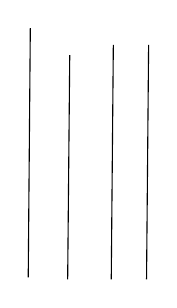
\begin{tikzpicture}[x=0.75pt,y=0.75pt,yscale=-1,xscale=1]
    %uncomment if require: \path (0,300); %set diagram left start at 0, and has height of 300
    
    %Straight Lines [id:da7690582805815367] 
    \draw    (201,99) -- (200,219) ;
    %Straight Lines [id:da936663735130838] 
    \draw    (220,112) -- (219,220) ;
    %Straight Lines [id:da7530223958992941] 
    \draw    (241,107) -- (240,220) ;
    %Straight Lines [id:da020592477605207327] 
    \draw    (258,107) -- (257,220) ;
    \end{tikzpicture}
\end{figure}

\underline{Problema:} Dado $G$, hallar un matching en $G$ con la mayor cantidad 
de lados posibles. Solo veremos matching en grafos bipartitos, como se muestra en 
figura de abajo.

\begin{figure}[h!]
    \centering
    \tikzset{every picture/.style={line width=0.75pt}} %set default line width to 0.75pt        
    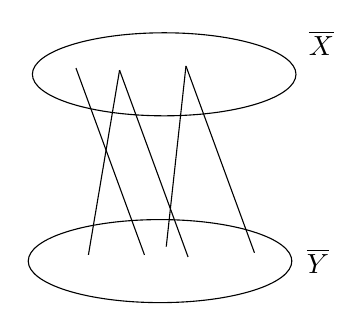
\begin{tikzpicture}[x=0.75pt,y=0.75pt,yscale=-1,xscale=1]
    %uncomment if require: \path (0,300); %set diagram left start at 0, and has height of 300

    %Straight Lines [id:da4723528897144176] 
    \draw    (225,77) -- (258,167) ;
    %Shape: Ellipse [id:dp5685481864376958] 
    \draw   (204,80) .. controls (204,68.95) and (232.43,60) .. (267.5,60) .. controls (302.57,60) and (331,68.95) .. (331,80) .. controls (331,91.05) and (302.57,100) .. (267.5,100) .. controls (232.43,100) and (204,91.05) .. (204,80) -- cycle ;
    %Shape: Ellipse [id:dp16624463198511918] 
    \draw   (202,170) .. controls (202,158.95) and (230.43,150) .. (265.5,150) .. controls (300.57,150) and (329,158.95) .. (329,170) .. controls (329,181.05) and (300.57,190) .. (265.5,190) .. controls (230.43,190) and (202,181.05) .. (202,170) -- cycle ;
    %Straight Lines [id:da5132940866558453] 
    \draw    (246,78) -- (231,167) ;
    %Straight Lines [id:da6633787446216199] 
    \draw    (246,78) -- (279,168) ;
    %Straight Lines [id:da7231441872259934] 
    \draw    (278,76) -- (311,166) ;
    %Straight Lines [id:da7002192762181896] 
    \draw    (278,76) -- (268.5,163) ;

    % Text Node
    \draw (336,57.8) node [anchor=north west][inner sep=0.75pt]    {$\overline{X}$};
    % Text Node
    \draw (335,162.8) node [anchor=north west][inner sep=0.75pt]    {$\overline{Y}$};
    \end{tikzpicture}
\end{figure}

Reduciremos el problema a un problema de flujo maximal. Tenemos que transformar un 
grafo bipartito $G$ en partes de $\bar{X}$ y $\bar{Y}$, en un network. Los vertices 
del network serán $\llaves{s,t} \cup \bar{X} \cup \bar{Y}$, y los lados 
$\llaves{\overrightarrow{xy}: x\in \bar{X}, y\in \bar{Y}, xy\in E} \cup \llaves{\overrightarrow{sx}: x\in \bar{X}} \cup \llaves{\overrightarrow{yt}: y\in \bar{Y}}$. Y 
las capacidades de los vertices son todas $1$. Ejemplo:

\begin{figure}[h!]
    \centering
    \tikzset{every picture/.style={line width=0.75pt}} %set default line width to 0.75pt        
    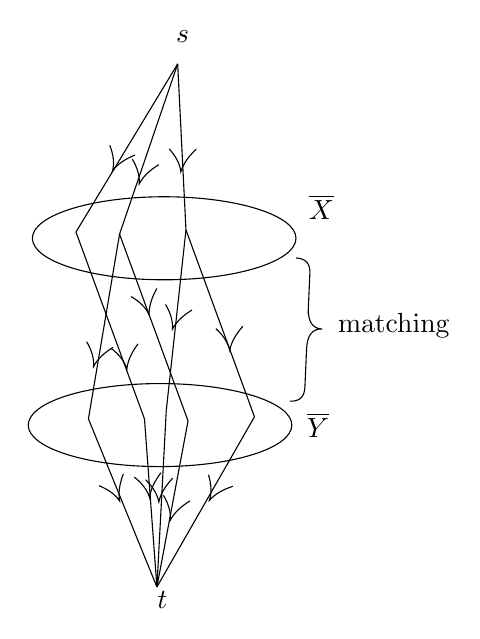
\begin{tikzpicture}[x=0.75pt,y=0.75pt,yscale=-1,xscale=1]
    %uncomment if require: \path (0,345); %set diagram left start at 0, and has height of 345
    %Straight Lines [id:da4723528897144176] 
    \draw    (233,116) -- (266,206) ;
    %Shape: Ellipse [id:dp5685481864376958] 
    \draw   (212,119) .. controls (212,107.95) and (240.43,99) .. (275.5,99) .. controls (310.57,99) and (339,107.95) .. (339,119) .. controls (339,130.05) and (310.57,139) .. (275.5,139) .. controls (240.43,139) and (212,130.05) .. (212,119) -- cycle ;
    %Shape: Ellipse [id:dp16624463198511918] 
    \draw   (210,209) .. controls (210,197.95) and (238.43,189) .. (273.5,189) .. controls (308.57,189) and (337,197.95) .. (337,209) .. controls (337,220.05) and (308.57,229) .. (273.5,229) .. controls (238.43,229) and (210,220.05) .. (210,209) -- cycle ;
    %Straight Lines [id:da5132940866558453] 
    \draw    (254,117) -- (239,206) ;
    %Straight Lines [id:da6633787446216199] 
    \draw    (254,117) -- (287,207) ;
    %Straight Lines [id:da7231441872259934] 
    \draw    (286,115) -- (319,205) ;
    %Straight Lines [id:da7002192762181896] 
    \draw    (286,115) -- (276.5,202) ;
    %Straight Lines [id:da5648258187550763] 
    \draw    (282,35) -- (233,116) ;
    %Straight Lines [id:da9766449049879795] 
    \draw    (282,35) -- (254,117) ;
    %Straight Lines [id:da06551185541471649] 
    \draw    (282,35) -- (286,115) ;
    %Straight Lines [id:da3852349618768396] 
    \draw    (239,206) -- (272,287) ;
    %Straight Lines [id:da2858395024028979] 
    \draw    (266,206) -- (272,287) ;
    %Straight Lines [id:da2559470060990032] 
    \draw    (276.5,202) -- (272,287) ;
    %Straight Lines [id:da5993012387391004] 
    \draw    (287,207) -- (272,287) ;
    %Straight Lines [id:da11346550360025387] 
    \draw    (319,205) -- (272,287) ;
    \draw   (308.61,238.48) .. controls (303.53,240.13) and (299.75,242.41) .. (297.28,245.3) .. controls (298.44,241.79) and (298.28,237.66) .. (296.82,232.92) ;
    \draw   (272.91,83.54) .. controls (268.35,86.33) and (265.2,89.42) .. (263.47,92.8) .. controls (263.78,89.12) and (262.67,85.14) .. (260.15,80.86) ;
    \draw   (261.45,78.88) .. controls (256.49,80.89) and (252.88,83.42) .. (250.63,86.48) .. controls (251.54,82.9) and (251.09,78.79) .. (249.29,74.16) ;
    \draw   (290.98,76.06) .. controls (287.05,79.69) and (284.57,83.34) .. (283.54,87) .. controls (283.13,83.33) and (281.25,79.64) .. (277.94,75.94) ;
    \draw   (313.41,161.4) .. controls (309.86,165.4) and (307.75,169.28) .. (307.08,173.02) .. controls (306.31,169.4) and (304.09,165.92) .. (300.42,162.56) ;
    \draw   (288.91,153.54) .. controls (284.35,156.33) and (281.2,159.42) .. (279.47,162.8) .. controls (279.78,159.12) and (278.67,155.14) .. (276.15,150.86) ;
    \draw   (250.91,171.54) .. controls (246.35,174.33) and (243.2,177.42) .. (241.47,180.8) .. controls (241.78,177.12) and (240.67,173.14) .. (238.15,168.86) ;
    \draw   (262.89,169.9) .. controls (259.68,174.18) and (257.89,178.21) .. (257.53,181.99) .. controls (256.47,178.45) and (253.97,175.16) .. (250.05,172.11) ;
    \draw   (271.97,143.19) .. controls (269.35,147.85) and (268.11,152.08) .. (268.25,155.88) .. controls (266.73,152.51) and (263.82,149.57) .. (259.53,147.06) ;
    \draw   (287.91,245.54) .. controls (283.35,248.33) and (280.2,251.42) .. (278.47,254.8) .. controls (278.78,251.12) and (277.67,247.14) .. (275.15,242.86) ;
    \draw   (279.58,234.59) .. controls (275.92,238.48) and (273.7,242.3) .. (272.93,246.02) .. controls (272.25,242.38) and (270.13,238.84) .. (266.57,235.38) ;
    \draw   (273.96,231.96) .. controls (270.7,236.21) and (268.87,240.22) .. (268.47,244) .. controls (267.45,240.45) and (264.98,237.13) .. (261.09,234.04) ;
    \draw   (255.81,232.52) .. controls (253.92,237.52) and (253.33,241.89) .. (254.05,245.62) .. controls (252.03,242.53) and (248.71,240.06) .. (244.1,238.23) ;
    %Shape: Brace [id:dp04371001661242979] 
    \draw   (336,197.5) .. controls (340.66,197.7) and (343.09,195.47) .. (343.3,190.81) -- (344.1,172.39) .. controls (344.39,165.73) and (346.86,162.5) .. (351.53,162.71) .. controls (346.86,162.5) and (344.68,159.07) .. (344.97,152.41)(344.84,155.41) -- (345.69,135.8) .. controls (345.89,131.13) and (343.66,128.7) .. (339,128.5) ;
    % Text Node
    \draw (344,96.8) node [anchor=north west][inner sep=0.75pt]    {$\overline{X}$};
    % Text Node
    \draw (343,201.8) node [anchor=north west][inner sep=0.75pt]    {$\overline{Y}$};
    % Text Node
    \draw (280,17.8) node [anchor=north west][inner sep=0.75pt]    {$s$};
    % Text Node
    \draw (271,287.8) node [anchor=north west][inner sep=0.75pt]    {$t$};
    % Text Node
    \draw (358,154) node [anchor=north west][inner sep=0.75pt]   [align=left] {matching};
    \end{tikzpicture}
\end{figure}

\underline{Propiedad:} Flujos enteros maximales en ese network se corresponden 
con matching maximales en $G$.
\medskip

\underline{Prueba:} Dado un flujo $f$ (maximal entero o no) en el network definimos:
\begin{align*}
    M_{f} = (V_{f}, E_{f})\,\, \text{con}\,\, V_{f} &= \llaves{v \in V: n_{f}(v)=1}\\
    E_{f} &= \llaves{xy, x\in \bar{X}, y\in \bar{Y}: f(xy)=1}
\end{align*}

\underline{$M_{f}$ es un matching} Sea $v \in V_{q}$. Si $v \in \bar{X}$, supongamos 
que $\delta_{M}(v) \neq 1$, pero $v\in V_{f} \Rightarrow In_{f}(v)=1 \Rightarrow out_{f}(v)=1$.
$\Rightarrow \exists y \in \bar{Y}: f(\overrightarrow{xy}) = 1 \Rightarrow In_{f}(y)=1$.
(observacion: como $f$ es entero y $c=1$ entonces $In_{f}(v)=0$ ó $1\,\, \forall v \neq s,t$)
\medskip

Entonces $y\in V_{f}$ y $vy \in E_{f} \Rightarrow \delta_{M_{f}}(v) \> 1$. Sino es $1$,
entonces $\exists z \neq y: vz \in E_{f} \Rightarrow f(\overrightarrow{vz}) = 1 \Rightarrow out_{f}(v) \> f(\overrightarrow{vy}) + f(\overrightarrow{vz}) = 2$.
Lo que es un absurdo, pues $in_{f}(v) = 1$.
\medskip

Entonces $\delta_{M}(v) =1, \,\, \forall v\in V_{f} \cap \bar{X}$.
\medskip

De la misma forma lo demostramos si $v \in \bar{Y}$.
$In_{f}(v)=1 \Rightarrow \exists x\in \bar{X}: f(\overrightarrow{xv}) = 1 \Rightarrow \delta_{M}(v) \> 1$ 
y si fuera $2$ o más $\exists x \neq x: f(\overrightarrow{zv}) =1 \Rightarrow In_{f}(v) \> 2$ Absurdo.
\medskip

Por lo tanto $M_{f}$ es un matching. Entonces:
\begin{align*}
    |E_{M_{f}}|&=\# \llaves{xy\in E_{f}}\,\, \text{como es un matching}\\
    &=\# \llaves{x \in \bar{X}: In_{f}(x)=1} = out_{f}(s) = v(f)\\
\end{align*}

Y viceversa, sea $M$ un matching en $G$ y definimos:
$$f(\overrightarrow{xy})= \left\{ \begin{array}{lcc}
    1 & \to & xy \in E(M)\\
    \\ 0& \to & \text{c.c.}\\
    \end{array}
    \right.$$

$$f(\overrightarrow{yt})= \left\{ \begin{array}{lcc}
    1 & \to & y \in V(M) \cap \bar{Y}\\
    \\ 0& \to & \text{c.c.}\\
    \end{array}
    \right.$$

$$f(\overrightarrow{sx})= \left\{ \begin{array}{lcc}
    1 & \to & xy \in V(M) \cup \bar{X}\\
    \\ 0& \to & \text{c.c.}\\
    \end{array}
    \right.$$

\begin{definition} Si $W \subseteq V$, entonces
    \begin{align*}
        \Gamma(\bar{W}) &= \llaves{z: \exists w \in \bar{W}: zw\in E}\\
        &= \cup_{w\in \bar{W}} \Gamma(w)\\
    \end{align*}
\end{definition}

\begin{definition} Un matching $M=(V_{M}, E_{M})$ en $G$ es perfecto si $V_{M} = V(G)$ 
    (si sus vertices coinciden con los de $G$).
\end{definition}

\begin{definition} (matching completo) Si $G = (\bar{X} \cup \bar{Y}, E)$ es bipartito. 
    Un matching $M = (V_{M}, E_{M})$ es completo de $\bar{X} \cap \bar{Y}$ si $V_{M} \cap \bar{X} = \bar{X}$.
\end{definition}

\subsection{Teorema de Hall}
\begin{teorema} (Hall) Si $G = (\bar{X} \cup \bar{Y}, E)$ es bipartito con partes 
    $\bar{X}$ e $\bar{Y}$, entonces existe matching completo de $\bar{X}$ en $\bar{Y}$
    si y solo si $|S| \< |\Gamma(S)| \,\, \forall S \subseteq \bar{X}$.
\end{teorema}

\underline{Prueba:}
\medskip

$(\Rightarrow)$ Si existe un matching completo de $\bar{X}$ en $\bar{Y}$, el matching 
induce una función inyectiva de $\bar{X} \cap \bar{Y}$ tal que $\psi(x) \in E$, por lo tanto:
$$\psi(S) \subseteq \Gamma(S)$$

por lo tanto, $|\Gamma(S)| \> |\psi(S)| = |S|$
\medskip

$(\Leftarrow)$ Queremos ver que si $\underbrace{|S| \< |\Gamma(S)|}_{P} \Rightarrow \underbrace{\exists\,\, \text{un matching completo de $\bar{X} \cap \bar{Y}$}}_{Q}$.
\medskip

Lo veremos de la siguiente forma $[P \Rightarrow Q] = [\neg Q \Rightarrow \neg P]$ 
por contrareciproca.
\medskip

Probaremos que sino existe matching entonces no se cumple Hall.
\medskip

\textbf{Si $\nexists$ matching completo de $\bar{X}$ en $\bar{Y}$, entonces al correr el 
algoritmo llegamos a un matching maximal que no cubre a $\bar{X}$}. Que es equivalente a 
hallar un flujo maximal entero $f$ cuyo valor no es $|\bar{X}|$.
\medskip

Al hallar $f$, también hallamos un corte minimal que vamos a denotar por $c$ (seria 
la última cola, la correr E-K).
\medskip

Sea $S = c \cap \bar{X}$, $T = c \cap \bar{Y}$, como en la siguiente imagen.
\begin{figure}[h!]
    \centering
    \tikzset{every picture/.style={line width=0.75pt}} %set default line width to 0.75pt        

    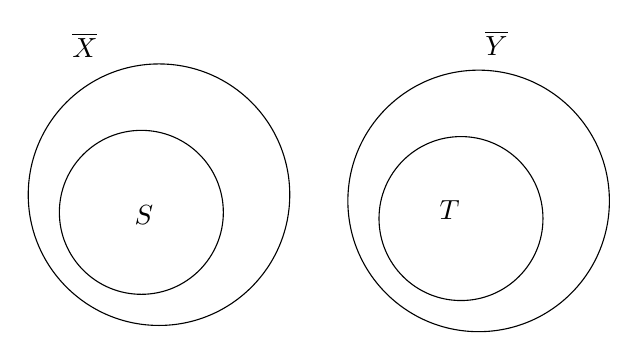
\begin{tikzpicture}[x=0.75pt,y=0.75pt,yscale=-1,xscale=1]
    %uncomment if require: \path (0,345); %set diagram left start at 0, and has height of 345
    
    %Shape: Circle [id:dp14718267969579513] 
    \draw   (118,156) .. controls (118,121.21) and (146.21,93) .. (181,93) .. controls (215.79,93) and (244,121.21) .. (244,156) .. controls (244,190.79) and (215.79,219) .. (181,219) .. controls (146.21,219) and (118,190.79) .. (118,156) -- cycle ;
    %Shape: Circle [id:dp9130235045197983] 
    \draw   (133,164.5) .. controls (133,142.68) and (150.68,125) .. (172.5,125) .. controls (194.32,125) and (212,142.68) .. (212,164.5) .. controls (212,186.32) and (194.32,204) .. (172.5,204) .. controls (150.68,204) and (133,186.32) .. (133,164.5) -- cycle ;
    %Shape: Circle [id:dp5449515002070981] 
    \draw   (272,159) .. controls (272,124.21) and (300.21,96) .. (335,96) .. controls (369.79,96) and (398,124.21) .. (398,159) .. controls (398,193.79) and (369.79,222) .. (335,222) .. controls (300.21,222) and (272,193.79) .. (272,159) -- cycle ;
    %Shape: Circle [id:dp4453429157761797] 
    \draw   (287,167.5) .. controls (287,145.68) and (304.68,128) .. (326.5,128) .. controls (348.32,128) and (366,145.68) .. (366,167.5) .. controls (366,189.32) and (348.32,207) .. (326.5,207) .. controls (304.68,207) and (287,189.32) .. (287,167.5) -- cycle ;
    
    % Text Node
    \draw (138,76.8) node [anchor=north west][inner sep=0.75pt]    {$\overline{X}$};
    % Text Node
    \draw (337,75.8) node [anchor=north west][inner sep=0.75pt]    {$\overline{Y}$};
    % Text Node
    \draw (168,159.8) node [anchor=north west][inner sep=0.75pt]    {$S$};
    % Text Node
    \draw (315,157.8) node [anchor=north west][inner sep=0.75pt]    {$T$};
    
    
    \end{tikzpicture}
\end{figure}

Entonces, $T$ forma parte de $c$ 
por lo tanto forma parte de la última cola. Entonces todos sus elementos fueron agregados 
por alguien (pues $S \notin T$), ese alguien debe ser vecino, y como el grafo es bipartito 
y $T \subseteq \bar{Y}$, esos vecinos deben estar en $\bar{X}$.
\medskip

Pero además deben hacer estado en la cola, es decir, que están en $c$. Entonces 
el vecino estaba en $S$. En resumen:
\medskip

$\forall y\in T, \exists x\in S: xy \in E \Rightarrow$ si $xy$ es lado $\Rightarrow$
$y$ es vecino $x$ con $x\in S$. Entonces, $y\in \Gamma(x) \subseteq \Gamma(S) \Rightarrow$
\begin{equation}
    T \subseteq \Gamma(S)
    \label{eq:1hall}
\end{equation}
Pero además:
\begin{equation}
    \Gamma(S) \subseteq T
    \label{eq:2hall}
\end{equation}

Ahora probemos \ref{eq:2hall}:
\medskip

Sea $y\in \Gamma(S) \Rightarrow \exists x\in S: xy\in E$ ($x$ esta en la cola).
\medskip

Supongamos que si $f(\overrightarrow{xy}) = 0$ entonces $x$ puede agregar a $y$ a la 
cola entonces $y \in T$.
\medskip

Supongamos que si $f(\overrightarrow{xy}) = 1$ entonces $x$ no puede agregar a $y$ a la 
cola pero $x\in S$ entonces algún vertice $z$ agrego a $x$ a la cola.
\medskip

Como $f(\overrightarrow{xy}) = 1$ entonces $out_{f}(x)=1 \Rightarrow In_{f}(x)=1 \Rightarrow f(\overrightarrow{sx})=1$.
Entonces, $s$ no agrego a $x$ a la cola por lo que $z \neq s$.
\medskip

Como $z$ debe ser un vecino de $x$ y $z \neq s$ entonces $z \in Y$. Y para agregar a $x$, 
lo debe haber hecho backward, entonces $f(\overrightarrow{xz})=1$ sino no puede. Entonces:
$f(\overrightarrow{xy})=1$ y $f(\overrightarrow{xz}) = 1$, por lo que $y=z$.
\medskip

Pero si $y=z$, agrego a $x$ a la cola, y esta en $c$, entonces $y\in c \cap Y = T$, 
con esto \ref{eq:2hall} queda demostrado.
\medskip

Además, \ref{eq:1hall} y \ref{eq:2hall} $\Rightarrow$ 
\begin{equation}
    T = \Gamma(S)
    \label{eq:3hall}
\end{equation}

Sea $S_{0} = \llaves{x\in \bar{X}: In_{f}(x)=0}$, entonces $s$ agrega a los vertices 
de $S_{0}$ a la cola, entonces:
\begin{equation}
    S_{0} \subseteq S
    \label{eq:4hall}
\end{equation}

Como estamos suponiendo que $v(f) \neq |x|$, entonces:
\begin{equation}
    S_{0} \neq \emptyset
    \label{eq:5hall}
\end{equation}
(me queda al menos un vertice sin matchear).
\medskip

Queremos comparar $S - S_{0}$ con $T$.
\medskip

$y\in T \Leftrightarrow y$ es puesto en la cola por alguien pero como $t\notin c$, 
y no puede poner a $t$. Entonces, $f(\overrightarrow{yt})=1 \Rightarrow out_{f}(y)=1$ 
y $In_{f}(y)=1$. Entonces $\exists x: f(\overrightarrow{xy})=1$.
\medskip

Como $f(\overrightarrow{xy})=1$ entonces, $y$ agrega a $x$ a la cola y $x\in S$ además 
$out_{f}(x) =1 \Rightarrow In_{f}(x)=1 \Rightarrow x \notin S_{0}$. Entonces, podemos 
concluir que $x\in S-S_{0}$. Y hay un solo $x$ con $f(\overrightarrow{xy})=1$.
\medskip

Entonces, tengo una función $y\to x$ y $T$ a $S-S_{0}$ inyectiva, pero además 
si $x\in S-S_{0}$ entonces $in_{f}(x)=1 \Rightarrow out_{f}(x)=1 \Rightarrow \exists y: f(\overrightarrow{xy})=1$.
\medskip

Entonces $y\in \Gamma(S) = T$ entonces tengo una biyección entre 
\begin{equation}
    T y S-S_{0}
    \label{eq:6hall}
\end{equation}
Finalmente:

\begin{equation}
    |\Gamma(S)| \underbrace{=}_{\ref{eq:3hall}} |T| \underbrace{=}_{\ref{eq:6hall}} = |S-S_{0}| \underbrace{=}_{\ref{eq:4hall}} |S| - |S_{0}| < |S|
\end{equation}

\subsection{Teorema del matrimonio de konig}
\begin{teorema} (matrimonio de konig) Todo grafo bipartito regular tiene un matching 
    perfecto (todos los vertices dorman parte del matching).
\end{teorema}

\underline{Prueba:} Dado un conjunto de vertices definimos:

$$E_{w} = \llaves{zw\in E: z\in W}$$

Sean $\bar{X}$ e $\bar{Y}$ las partes de $G$ y supongamos $w \subseteq \bar{X}$ 
(completamente contenido en $\bar{X}$). Entonces:
\begin{align*}
    |E_{w}| &= |\llaves{xw: x\in W}| \\
    &\text{Como $w \subseteq \bar{X}$ y no hay lados entre vertices de $\bar{X}$},\\ 
    &\text{cada lado que aparece en $E_{w}$, aparece una sola vez} \\
    &=\sum_{x\in W} |\Gamma(x)|\\
    &=\sum_{x\in W} \delta(x)\\
    &\text{Como $G$ es regular}\\
    &\sum_{x\in W} \Delta = \Delta |W|
\end{align*}
Si $W \subseteq Y$ vale el mismo analisis y tambien tenemos que $|G_{w}| = \Delta |W|$.
\medskip

Primero demostraremos que hay un matching completo (basta demostrar la condición de Hall).
\medskip

Sea $S \subseteq \bar{X}$ y sea $l \in E_{s}$, entonces $l$ es de la forma $l=xy$ con 
$x\in S$ y $y\in W$. Como $l$ es lado, entonces $y$ es vecino de $x$ entonces $y\in \Gamma(x)$. 
Pero $x\in S \Rightarrow y\in \Gamma(S)$. Como $l=xy$ entonces si $y\in \Gamma(S) \Rightarrow l\in E_{\Gamma(S)}$.
\medskip

Conclusión: $E_{S} \subseteq E_{\Gamma(S)} \Rightarrow |E_{s}| \< |E_{\Gamma(S)}|$. Y 
como $S \subseteq X \Rightarrow |E_{S}| = \Delta |S|$. A su vez, $\Gamma(S) \subseteq Y \Rightarrow |E_{\Gamma(S)}| = \Delta |\Gamma(S)|$. 
Entonces podemos decir que $\cancel{\Delta} |S| \< \cancel{\Delta} |\Gamma(S)| \Rightarrow |S| \< |\Gamma(S)|$.
\medskip

Entonces se satisface la condición de Hall, entonces podemos afirmar que existe matching compreto 
de $x$ a $y$. Para ver que ese matching es perfecto basta ver que $|\bar{X}| = |\bar{Y}|$.
\medskip

Como $G$ es bipartito los unicos lados son entre $x$ e $y$. Entonces:
\begin{align*}
    E &= E_{\bar{X}} + E_{\bar{Y}}\\
    &\text{Por lo tanto}\\
    &|E_{\bar{X}}| = |E_{\bar{Y}}|\\
    &\text{Como $G$ es regular}\\
    &\Delta |\bar{X}| = \Delta |\bar{Y}|\\
    &|\bar{X}| = |\bar{Y}|
\end{align*}

\begin{corolario} (tambien de koring) $G$ bipartito entonces $\chi^{'}(G) = \Delta(G)$.
\end{corolario}

Donde $\chi^{'}(G)$ es el indice cromatico (lados del un grafo), osea, la menor 
cantidad de colores necesarios para colorear los lados de un grafo de forma tal 
que lados con un vertice en común tengan colores distintos. Es obvio que $\Delta \< \chi^{'}(G)$.
\medskip

\underline{Prueba:} Supongamos $G$ regular, por el teorema del matrimonio $G$ 
tiene un matching perfecto (puedo colorear a todos con un color color sin 
ningún problema, ej. puedo usar el color $1$).
\medskip

Luego remuevo los lados, entonces $\widetilde{G} = G -\text{esos lados}$, cada 
vertice disminuye su grado en $1$. Entonces $\widetilde{G}$ siguie siendo regular. 
Por lo que tiene un matching perfecto. Coloreo esos lados con el color $2$, los remuevo, etc.
\medskip

Siempre va a ser regular hasta el final y terminamos coloreando con $\Delta$ colores. 
Qué pasa si $G$ no es regular?

\begin{lema} $G$ bipartito, entonces existe $H$ bipartito regular tal que 
    $G \subseteq H$. Entonces $\Delta(G) = \Delta(H)$.
\end{lema}

Entonces $\chi^{'}(H) = \Delta$. $G \subseteq H \Rightarrow \chi^{'}(G) \< \Delta$. 
Como $\Delta \< \chi^{'}(G) \Rightarrow \chi^{'}(G) = \Delta$.

\section{Matchings con pesos: Minimizar la suma}

\underline{Observaciones triviales:} si $A$ tiene entrada no negativa tal que 
exista un matching de ceros, es decir, un matching donde todas las entradas correspondientes 
al matching son ceros.
\medskip

Entonces ese matching minimiza la suma, pues la suma da $0$ y cualquier otro matching 
tiene suma mayor o igual a $0$.

\begin{lema} Sea $A$ una matriz de pesos ($n\times n$). Sea $\widetilde{A}$ la matriz 
    que se obtienen de $A$ restando una constante a cada entrada de una sola fila o 
    columna de $A$. Entonces un matching minimiza la suma relativa a $A$ sii la 
    minimiza (la suma) relativa a $\widetilde{A}$.
\end{lema}
\underline{Prueba:}
\medskip

Observemos que un matching da origen a una permutación de $\llaves{1,2,\dots,n}$, y 
viceversa. Sea $\sigma$ la permutación correspondiente a un matching $M$ 
(que puede no minimizar la suma). Entonces la suma correspondiente al matching $M$, 
relativa a $A$ es:
$$S = \sum_{i=1}^{n} A_{i,\sigma(i)}$$

y relativa a $\widetilde{A}$ es:
$$\widetilde{S} = \sum_{i=1}^{n} \widetilde{A}_{i,\sigma(i)}$$

$\widetilde{A}$ se obtiene de $A$ restando una constante $c$ de alguna fila o columna 
de $A$ para concretar supongamos que es la fila $k$. Entonces:
$$\widetilde{A}_{i,j}= \left\{ \begin{array}{lcc}
    A_{i,j} & si & i \neq k\\
    \\ A_{k,j} & si & i = k\\
    \end{array}
    \right.$$

Entonces:
\begin{align*}
    \widetilde{S} = \sum_{i=1}^{n} A_{i,\sigma(i)} &= \parent{\sum_{i\neq k} \widetilde{A}_{i,\sigma(i)}} + \widetilde{A}_{k,\sigma(k)}\\
    &= \parent{\sum_{i\neq k} A_{i,\sigma(i)}} + A_{k,\sigma(k)} - c\\
    &= \parent{\sum_{i=1}^{n} A_{i,\sigma(i)}} - c\\
    &= S - c
\end{align*}

Entonces si $M_{1}$ y $M_{2}$ son matchings y denotamos sus sumas por $S_{1}, \widetilde{S}_{1}, S_{2}, \widetilde{S}_{2}$ 
respectivamente tenesmos que:
$$\widetilde{S}_{1} \subseteq \widetilde{S}_{2} \Leftrightarrow S_{1} - x \< S_{2} - c \Leftrightarrow S_{1} \< S_{2}$$

\underline{Complejidad de los algoritmos de matchings:}
\begin{itemize}
    \item [1.] Algoritmo de hallar matching maximal:
    
    - Matching inicial, revisar cada fila es $O(n)$, como hay $n$ filas entonces es $O(n^{2})$.
    
    - Extender el matching en un lado, es le mismo análisis entonces es $O(n^{2})$.
    
    - Hay $O(n)$ extensiones de matching.

    Entonces la complejidad total es $O(n^{2})*O(n) = O(n^{3})$.

    Si se hace con Dinitz se puede ver que es $O(n^{2.5})$ (si o si leer el network).

    \item [2.] Minimizar el maximo:
    
    - Ordenar las $n^{2}$ entradas, es $O(n^{2}log(n^{2})) = O(n^{2}log(n))$.

    - Hay que hacer (usando busqueda binaria). Entonces es $O(log(n^{2}))$ el algoritmo 
    de hallar matching maximal. 

    Entonces la complejidad total es $O(n^{3}log(n))$ o $O(n^{2.5}log(n))$ si lo hicieramos con Dinitz.

    \item [3.] Minimizar la suma (algoritmo de Kuhn-Munkres o hungaro):
    \begin{lema} Luego de que el algoritmo realiza un cambio de matriz asociado a un $S$
        $(|S| > \Gamma(S)|)$, si se sigue corriendo el algoritmo a partir del matching 
        parcial que se tenia, entonces crece el matching o crece $S$.
    \end{lema}
    \underline{Prueba:}
    \medskip

    Al cambiar la matriz, sumamos $m = \min \llaves{S \times \Gamma(S)}$ y restamos 
    $m$ de $S$, sumamos $m$ a $\Gamma(S)$.

    Primero repasemos un poco:
    \begin{itemize}
        \item [1)] Qué constante restar/sumar?
        \item [2)] Queda una matriz de entradas no negativas?
    \end{itemize}

    Queremos al menos un nuevo cero, pero que no queden entradas negativas, inicialmente tenemos:
    \begin{figure}[h!]
        \centering
        \tikzset{every picture/.style={line width=0.75pt}} %set default line width to 0.75pt        
        \begin{tikzpicture}[x=0.75pt,y=0.75pt,yscale=-1,xscale=1]
        %uncomment if require: \path (0,345); %set diagram left start at 0, and has height of 345
        %Straight Lines [id:da3728708647629504] 
        \draw    (79,30) -- (80,162) ;
        %Straight Lines [id:da3538000297098778] 
        \draw    (220,30) -- (219,163) ;
        %Straight Lines [id:da5213754633276941] 
        \draw    (56,61) -- (257,63) ;
        %Straight Lines [id:da2635360079116318] 
        \draw    (175,190) -- (175,23) ;
        %Shape: Brace [id:dp504617179785745] 
        \draw   (266,164) .. controls (270.67,163.95) and (272.98,161.6) .. (272.93,156.93) -- (272.6,124.93) .. controls (272.53,118.26) and (274.83,114.91) .. (279.5,114.86) .. controls (274.83,114.91) and (272.47,111.6) .. (272.4,104.93)(272.43,107.93) -- (272.08,72.93) .. controls (272.03,68.26) and (269.68,65.95) .. (265.01,66) ;
        %Curve Lines [id:da21047916805321942] 
        \draw    (122,42) .. controls (147.74,22.7) and (224.82,15.81) .. (284.78,33.34) .. controls (317.33,42.86) and (344.83,59.58) .. (356.32,85.41) ;
        \draw [shift={(357,87)}, rotate = 247.54] [color={rgb, 255:red, 0; green, 0; blue, 0 }  ][line width=0.75]    (10.93,-3.29) .. controls (6.95,-1.4) and (3.31,-0.3) .. (0,0) .. controls (3.31,0.3) and (6.95,1.4) .. (10.93,3.29)   ;
        %Curve Lines [id:da5979183966121386] 
        \draw    (188,126) .. controls (213.74,106.7) and (294.05,205.47) .. (354,223) .. controls (412.75,240.18) and (373.64,132.45) .. (360.75,107.43) ;
        \draw [shift={(360,106)}, rotate = 61.39] [color={rgb, 255:red, 0; green, 0; blue, 0 }  ][line width=0.75]    (10.93,-3.29) .. controls (6.95,-1.4) and (3.31,-0.3) .. (0,0) .. controls (3.31,0.3) and (6.95,1.4) .. (10.93,3.29)   ;
        % Text Node
        \draw (87,84.8) node [anchor=north west][inner sep=0.75pt]    {$No\ hay\ ceros$};
        % Text Node
        \draw (108,136.8) node [anchor=north west][inner sep=0.75pt]    {$\overline{\Gamma ( S)}$};
        % Text Node
        \draw (182,150.8) node [anchor=north west][inner sep=0.75pt]    {$\Gamma ( S)$};
        % Text Node
        \draw (286,106.8) node [anchor=north west][inner sep=0.75pt]    {$S$};
        % Text Node
        \draw (359,89.8) node [anchor=north west][inner sep=0.75pt]    {$Aca\ estan\ los\ ceros\ del\ matching$};
        \end{tikzpicture}
    \end{figure}

    Como $\Gamma(S) = \text{vecinos de S}$, en el conjunto $\overline{\Gamma(S)}$ no hay ceros,
    en la fila de $S$, es decir, en $S\times \Gamma(S)$ no hay ceros. Entonces, al sumar $m$ 
    y restar los $m$ en $S$ (filas) y sumamos $m$ en $\Gamma(S)$ (columnas), como 
    se muestra acontinuación:
    \newpage
    \begin{figure}[h!]
        \centering
        \tikzset{every picture/.style={line width=0.75pt}} %set default line width to 0.75pt        
        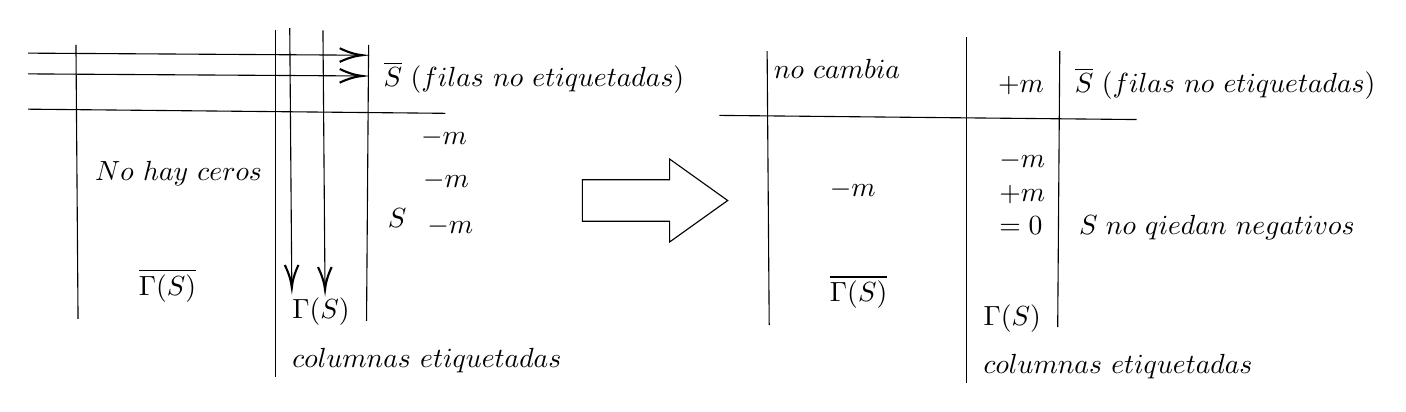
\begin{tikzpicture}[x=0.75pt,y=0.75pt,yscale=-1,xscale=1]
        %uncomment if require: \path (0,345); %set diagram left start at 0, and has height of 345
        %Straight Lines [id:da7621214744983624] 
        \draw    (29,22) -- (30,154) ;
        %Straight Lines [id:da3228432102557248] 
        \draw    (170,22) -- (169,155) ;
        %Straight Lines [id:da2616205007188461] 
        \draw    (6,53) -- (207,55) ;
        %Straight Lines [id:da5101429907461392] 
        \draw    (125,182) -- (125,15) ;
        %Straight Lines [id:da6327284465087757] 
        \draw    (6,26) -- (165,26.99) ;
        \draw [shift={(167,27)}, rotate = 180.36] [color={rgb, 255:red, 0; green, 0; blue, 0 }  ][line width=0.75]    (10.93,-3.29) .. controls (6.95,-1.4) and (3.31,-0.3) .. (0,0) .. controls (3.31,0.3) and (6.95,1.4) .. (10.93,3.29)   ;
        %Straight Lines [id:da16803123210681292] 
        \draw    (6,36) -- (165,36.99) ;
        \draw [shift={(167,37)}, rotate = 180.36] [color={rgb, 255:red, 0; green, 0; blue, 0 }  ][line width=0.75]    (10.93,-3.29) .. controls (6.95,-1.4) and (3.31,-0.3) .. (0,0) .. controls (3.31,0.3) and (6.95,1.4) .. (10.93,3.29)   ;
        %Straight Lines [id:da26346681835575736] 
        \draw    (132,14) -- (132.98,137) ;
        \draw [shift={(133,139)}, rotate = 269.54] [color={rgb, 255:red, 0; green, 0; blue, 0 }  ][line width=0.75]    (10.93,-3.29) .. controls (6.95,-1.4) and (3.31,-0.3) .. (0,0) .. controls (3.31,0.3) and (6.95,1.4) .. (10.93,3.29)   ;
        %Straight Lines [id:da6754611104200088] 
        \draw    (148,15) -- (148.98,138) ;
        \draw [shift={(149,140)}, rotate = 269.54] [color={rgb, 255:red, 0; green, 0; blue, 0 }  ][line width=0.75]    (10.93,-3.29) .. controls (6.95,-1.4) and (3.31,-0.3) .. (0,0) .. controls (3.31,0.3) and (6.95,1.4) .. (10.93,3.29)   ;
        %Right Arrow [id:dp13027636235600637] 
        \draw   (273,87) -- (315,87) -- (315,77) -- (343,97) -- (315,117) -- (315,107) -- (273,107) -- cycle ;
        %Straight Lines [id:da5904443269843922] 
        \draw    (362,25) -- (363,157) ;
        %Straight Lines [id:da24213000279475994] 
        \draw    (503,25) -- (502,158) ;
        %Straight Lines [id:da3457300599456079] 
        \draw    (339,56) -- (540,58) ;
        %Straight Lines [id:da8432486889122361] 
        \draw    (458,185) -- (458,18) ;

        % Text Node
        \draw (37,76.8) node [anchor=north west][inner sep=0.75pt]    {$No\ hay\ ceros$};
        % Text Node
        \draw (58,128.8) node [anchor=north west][inner sep=0.75pt]    {$\overline{\Gamma ( S)}$};
        % Text Node
        \draw (132,142.8) node [anchor=north west][inner sep=0.75pt]    {$\Gamma ( S)$};
        % Text Node
        \draw (178,99.8) node [anchor=north west][inner sep=0.75pt]    {$S$};
        % Text Node
        \draw (176,28.8) node [anchor=north west][inner sep=0.75pt]    {$\overline{S}$};
        % Text Node
        \draw (189,30.8) node [anchor=north west][inner sep=0.75pt]    {$( filas\ no\ etiquetadas)$};
        % Text Node
        \draw (132,166.8) node [anchor=north west][inner sep=0.75pt]    {$columnas\ etiquetadas$};
        % Text Node
        \draw (194,60.8) node [anchor=north west][inner sep=0.75pt]    {$-m$};
        % Text Node
        \draw (195,81.8) node [anchor=north west][inner sep=0.75pt]    {$-m$};
        % Text Node
        \draw (197,103.8) node [anchor=north west][inner sep=0.75pt]    {$-m$};
        % Text Node
        \draw (391,131.8) node [anchor=north west][inner sep=0.75pt]    {$\overline{\Gamma ( S)}$};
        % Text Node
        \draw (465,145.8) node [anchor=north west][inner sep=0.75pt]    {$\Gamma ( S)$};
        % Text Node
        \draw (511,102.8) node [anchor=north west][inner sep=0.75pt]    {$S$};
        % Text Node
        \draw (509,31.8) node [anchor=north west][inner sep=0.75pt]    {$\overline{S}$};
        % Text Node
        \draw (522,33.8) node [anchor=north west][inner sep=0.75pt]    {$( filas\ no\ etiquetadas)$};
        % Text Node
        \draw (465,169.8) node [anchor=north west][inner sep=0.75pt]    {$columnas\ etiquetadas$};
        % Text Node
        \draw (472,35.8) node [anchor=north west][inner sep=0.75pt]    {$+m$};
        % Text Node
        \draw (466,68.8) node [anchor=north west][inner sep=0.75pt]    {$ \begin{array}{l}
        -m\\
        +m\\
        =0
        \end{array}$};
        % Text Node
        \draw (391,85.8) node [anchor=north west][inner sep=0.75pt]    {$-m$};
        % Text Node
        \draw (364,27.8) node [anchor=north west][inner sep=0.75pt]    {$no\ cambia$};
        % Text Node
        \draw (524,102.8) node [anchor=north west][inner sep=0.75pt]    {$no\ qiedan\ negativos$};
        \end{tikzpicture}
        \end{figure}

    Entonces, en el algoritmo al buscar nuevos ceros los tendremos en la siguiente
    región de la matriz:

        \begin{figure}[h!]
            \centering
            \tikzset{every picture/.style={line width=0.75pt}} %set default line width to 0.75pt        

            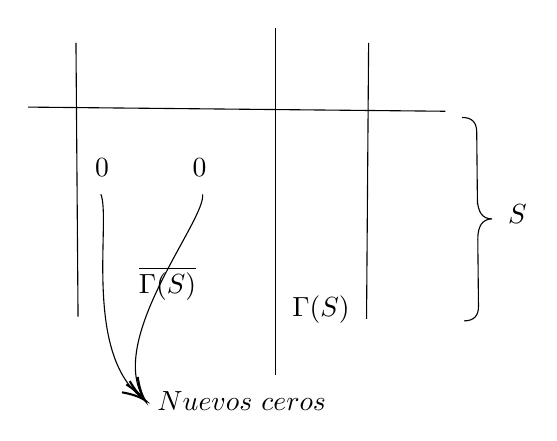
\begin{tikzpicture}[x=0.75pt,y=0.75pt,yscale=-1,xscale=1]
            %uncomment if require: \path (0,345); %set diagram left start at 0, and has height of 345

            %Straight Lines [id:da43671896021279566] 
            \draw    (79,30) -- (80,162) ;
            %Straight Lines [id:da7624681737268457] 
            \draw    (220,30) -- (219,163) ;
            %Straight Lines [id:da15351564236577664] 
            \draw    (56,61) -- (257,63) ;
            %Straight Lines [id:da9581191619998763] 
            \draw    (175,190) -- (175,23) ;
            %Shape: Brace [id:dp643775637620954] 
            \draw   (266,164) .. controls (270.67,163.95) and (272.98,161.6) .. (272.93,156.93) -- (272.6,124.93) .. controls (272.53,118.26) and (274.83,114.91) .. (279.5,114.86) .. controls (274.83,114.91) and (272.47,111.6) .. (272.4,104.93)(272.43,107.93) -- (272.08,72.93) .. controls (272.03,68.26) and (269.68,65.95) .. (265.01,66) ;
            %Curve Lines [id:da7441773535908995] 
            \draw    (91,103) .. controls (95.93,114.82) and (82.42,179.03) .. (110.68,201.02) ;
            \draw [shift={(112,202)}, rotate = 214.99] [color={rgb, 255:red, 0; green, 0; blue, 0 }  ][line width=0.75]    (10.93,-3.29) .. controls (6.95,-1.4) and (3.31,-0.3) .. (0,0) .. controls (3.31,0.3) and (6.95,1.4) .. (10.93,3.29)   ;
            %Curve Lines [id:da6037489259291242] 
            \draw    (140,103) .. controls (141.97,114.82) and (94.46,171.27) .. (111.19,200.68) ;
            \draw [shift={(112,202)}, rotate = 236.77] [color={rgb, 255:red, 0; green, 0; blue, 0 }  ][line width=0.75]    (10.93,-3.29) .. controls (6.95,-1.4) and (3.31,-0.3) .. (0,0) .. controls (3.31,0.3) and (6.95,1.4) .. (10.93,3.29)   ;

            % Text Node
            \draw (87,84.8) node [anchor=north west][inner sep=0.75pt]    {$0$};
            % Text Node
            \draw (108,136.8) node [anchor=north west][inner sep=0.75pt]    {$\overline{\Gamma ( S)}$};
            % Text Node
            \draw (182,150.8) node [anchor=north west][inner sep=0.75pt]    {$\Gamma ( S)$};
            % Text Node
            \draw (286,106.8) node [anchor=north west][inner sep=0.75pt]    {$S$};
            % Text Node
            \draw (134,84.8) node [anchor=north west][inner sep=0.75pt]    {$0$};
            % Text Node
            \draw (117,196.8) node [anchor=north west][inner sep=0.75pt]    {$Nuevos\ ceros$};
            \end{tikzpicture}
        \end{figure}
    Cualquier nuevo cero estará en $S\times \overline{\Gamma(S)}$. Supongamos que 
    está en la fila $i$, columna $j$, entonces $i \in S$ y $j\in \overline{\Gamma(S)}$
    (la columna $j$ no tiene etiqueta). Ese nuevo cero hará que etiquetemos la columna 
    $j$ con la etiquete $i$. Al chequear si la columna $j$ esta libre o forma parte 
    del matching, tenemos:
    \begin{itemize}
        \item [-] Si esta libre, entonces extendemos el matching por lo que crece.
        \item [-] Si forma parte del matching, existe una fila $k$ tal que $(k,j)$ es 
            parte del matching.
            
            En particular, $j$ es vecino de $k$. Entonces $k \notin S$, pues $j \notin \Gamma(S)$
            pero el algoritmo al chequear $j$ va a agregar a $k$ al nuevo $S$ por lo que $S$ crece.
            Como lo muesta la siguiente imagen.
            \begin{figure}[h!]
                \centering
                \tikzset{every picture/.style={line width=0.75pt}} %set default line width to 0.75pt        
                \begin{tikzpicture}[x=0.75pt,y=0.75pt,yscale=-1,xscale=1]
                %uncomment if require: \path (0,345); %set diagram left start at 0, and has height of 345

                %Straight Lines [id:da8372784341649588] 
                \draw    (79,30) -- (80,162) ;
                %Straight Lines [id:da5109874942006682] 
                \draw    (220,30) -- (219,163) ;
                %Shape: Rectangle [id:dp06089573648047919] 
                \draw   (132,70) -- (152,70) -- (152,88) -- (132,88) -- cycle ;
                %Straight Lines [id:da551912388218476] 
                \draw    (55,77) -- (132,77) ;
                %Straight Lines [id:da22608547891665576] 
                \draw    (152,77) -- (229,77) ;
                %Straight Lines [id:da22717619842304848] 
                \draw    (135,121) -- (222,121) ;
                %Straight Lines [id:da9916414867336225] 
                \draw    (57,121) -- (117,121) ;
                %Straight Lines [id:da0038770896514386255] 
                \draw    (127,160) -- (128,142) -- (128,129) ;

                % Text Node
                \draw (122,113.8) node [anchor=north west][inner sep=0.75pt]    {$0$};
                % Text Node
                \draw (134,72.8) node [anchor=north west][inner sep=0.75pt]    {$j$};
                % Text Node
                \draw (138,18.8) node [anchor=north west][inner sep=0.75pt]    {$j$};
                % Text Node
                \draw (234,69.8) node [anchor=north west][inner sep=0.75pt]    {$j$};
                % Text Node
                \draw (229,114.8) node [anchor=north west][inner sep=0.75pt]    {$i$};
                % Text Node
                \draw (123,161.8) node [anchor=north west][inner sep=0.75pt]    {$i$};
                % Text Node
                \draw (43,113.8) node [anchor=north west][inner sep=0.75pt]    {$i$};
                % Text Node
                \draw (44,68.8) node [anchor=north west][inner sep=0.75pt]    {$k$};
                \end{tikzpicture}
            \end{figure}
    \end{itemize}
    \begin{corolario} Puede haber a lo sumo $O(n)$ cambios de matriz. Antes de extender 
        el matching en un lado (pues $S$ puede crecer a lo sumo $O(n)$ veces).
    \end{corolario}
\end{itemize}

\subsection{Complejidad del algoritmo hungaro}
\begin{teorema} La complejidad del algoritmo Hungaro como lo vimos en clase es $O(n^4)$.
\end{teorema}

\underline{Prueba:} Resta el $min$ de una fila es $O(n)$, entonces restar $min$ de 
cada columna es $O(n^2)$. Mismo análisis para restar $min$ a cada columna es $O(n^{2})$.
\medskip

Hallar matching inicial es $O(n^2)$. Este matching se puede extender a los umo 
$O(n)$ veces. Por lo tanto:
$$\text{Complejidad Hungaro} = O(n^2) + O(n)*(\text{Complejidad de extender matching en un lado})$$

Para extender el matching, hay que revisar $m$ filas buscando ceros, entonces cada 
busqueda es $O(n)$.
\medskip

Luego revisar de revisar a lo sumo $n$ filas, si o si extendemos el matching pero 
en el medio quezas debamos hacer cambios de matrices, si seguimos con el matching 
parcial que teniamos, no hace falta re-escanear las filas de $S$ (esta dentro del 
cambio de matriz).
\medskip

Y además por le lema sabemos que hay $\< O(n)$cambios de matries antes de extender 
el matching. Por lo tanto:
$$\text{Complejidad de extender el matching en un lado} = \underbrace{O(n^{2})}_{\text{escanear filas}} + \underbrace{O(n)}_{\text{\# cambio de matrices}} + CCM$$

donde $CCM$ es la complejidad de hacer un cambio de matriz (esto pude cambiar al programarlo).
Entonces, cambiar la matriz requiere:
\medskip

\begin{itemize}
    \item [1.] Calcular $m = \min \llaves{S \times \Gamma(S)}$ (esto es $O(|S \times \Gamma(S)|)=O(n^2)$).
    \item [2.] Restar $m$ de $S$ (filas) esto es $O(n)*|S| = O(n^2)$. Sumar $m$ a $\Gamma(S)$ (columnas) 
        eso es $O(n)*|\Gamma(S)| = O(n^2)$.
\end{itemize}
Entonces:
$$CCM = O(n^2) + O(n^2) + O(n^2) = O(n^2)$$

Por lo tanto:
$$\text{Complejidad hungaro} = O(n^{2}) + O(n)*(O(n^{2}) + O(n)*O(n^{2})) = O(n^{4})$$

\begin{teorema} El hungaro se puede coficar en $O(n^3)$.
\end{teorema}
\underline{Prueba:}
\medskip

Hay que tratar de hacer que $CCM = O(n)$, entonces:
$$\text{Complejidad hungaro} = O(n^{2}) + O(n)*(O(n^{2}) + O(n)*O(n)) = O(n^{3})$$

Debemos:
\begin{itemize}
    \item [1.] Hallar un $min$ de $O(n^{2})$ elementos en $O(n)$.
    \item [2.] Debemo cambiar $O(n^{2})$ elementos en $O(n)$.
\end{itemize}

Para hacer $1.$ parte del costo de hallar cada $m$ se traslada a la parte donde 
escaneamos filas, entonces:
\begin{align*}
    m &= \min \llaves{S \times \Gamma(S)},\,\, \text{Sea $C$ la matriz de costos} \\
    &= \min \llaves{C_{x,y} : x \in S, y \notin \Gamma(S)} \\
    &= \min_{y\notin \Gamma(S)} \parent{\min_{x\in S}\llaves{C_{x,y}}}\,\,(\text{esto de puede calcular en $O(n)$ haciendo})\\
    &= \min_{y \notin \Gamma(S)} M_{y} 
\end{align*}

donde $M_{y} = \min_{x\in S}\llaves{C_{x,y}}$, siempre hay que tenerlo precalculado. Precalcular 
los $M_{y}$ demanda $O(n)$ pero los podemos hacer cuanod escanemos una fila al buscar 
ceto, en los no cero actualizamos $M_{y}$.
\medskip

Para $2.$ hacemos una resta y suma virtual (indicar cuanto se le deberia restar y sumar). 
Entonces usamos $RF(x)$ que indique cuanto restarle a la fila $x$ y $SC(x)$ que indique 
cuanto sumarle a la columna $y$.
\medskip

Restar $m$ de $S$ es simplemente hacer $RF(x) += m,\, \forall x\in S$ esto es $O(n)$.

Sumar $m$ a $\Gamma(S)$ es simplemente hacer $SC(y) += m,\, \forall y\in \Gamma(S)$ esto es $O(n)$.
\medskip

El problema es el chequeo de ceros. Entonces, en vez de hacer
\begin{lstlisting}[language=C]
    if(0 == C(x)(y))
\end{lstlisting}

se chequea haciendo:
\begin{lstlisting}[language=C]
    if(0 == C(x)(y) - RF(x) - SC(y))
\end{lstlisting}
que es $O(n)$.

\section{Códigos de corrección de errores}
Un código (binario de bloque) es un subconjunto de $\llaves{0,1}^{n}$ para algún 
$n$ fijo. Que sea en bloque quiere decir que todas las palabras tienen la misma
longitud.
\medskip

Suponemos que el medio de transmisión puede cambiar bits pero no agregar ni sustraer.
También suponemos que la probabilidad de cambiar $0 \to 1$ es igual a la de $1 \to 0$ 
es la misma para todos los bits, y e independiente entre los bits.
\medskip

Si a esa probabilidad la llamamos $p$, entonce $0 < p < \frac{1}{2}$. Y la probabilidad 
de $t$ errores es $p^{t}$.

\begin{definition} La distancia de hamming entre dos palabras $x,y\in \llaves{0,1}^{n}$ es:
    $$d_{H}(x,y) = \# \text{de bits de diferencia entre $x$ e $y$}$$
\end{definition}

\underline{Propiedad:} Como $d_{H}$ es una distancia, valen las siguientes propiedades:
\begin{itemize}
    \item [A)] $d_{H}(x,y) = d_{H}(y,x)$
    \item [B)] $d_{H}(x,y) \> 0$
    \item [C)] $d_{H}(x,y) = 0 \iff x = y$
    \item [D)] Desigualdad triangular: $d_{H}(x,y) \< d_{H}(x,z) + d_{H}(z,y)$
\end{itemize}

\subsection{Código de corrección de errores:}

\begin{definition} Sea $\delta = \delta(c) = \min \llaves{d_{H}(x,y): x,y\in C, x\neq y}$
\end{definition}

\begin{definition} Un código $C$ detecta $r$ errores.\\
    Si $D_{r}(x) \cap C = \llaves{x},\, \forall x\in C$ (detecta si hubo por lo menos 
    un error, pero no sabe cuantos.). Donde $D_{r}(x) = \llaves{y\in \llaves{0,1}^{n}: d_{H}(x,y) \< r}$.
    $C$ corrige $t$ errores si $D_{t}(x) \cap D_{y}(y) = \emptyset,\, \forall x,y \in C, x\neq y$
\end{definition}

\begin{teorema} Sea $C$ un código tal que $R$ es la mayor capacidad de detección 
    de errores de $C$, es decir, $C$ detecta $R$ errores pero no $R+1$ y $Q$ la 
    mayor capacidad de corrección de errores de $C$, es decir , $C$ corrige $Q$
    errores y no corrge $Q+1$ errores. Entonces:
    $R = \delta-1$ y $Q = \lfloor \frac{\delta-1}{2} \rfloor $
\end{teorema}
\underline{Prueba:}
\medskip

Sea $z\in D_{\delta -1}(x) \cap C$ para algún $x\in C$. Entonces como $z\in D_{\delta -1}(x)$
podemos decir que $d{H}(x,z) \< \delta -1$ por definición de disco.
\medskip

Como $x,z \in C$ entonces $x=z$ o $\delta \< d_{H}(x,z)$. Pero es un absurdo. Conclusión 
$x=z$ por lo tanto $D_{\delta -1}(x) \cap C = \llaves{x}$ y $C$ detecta $\delta -1$ errores.
\medskip

$C$ no detecta $\delta$ errores. Pues sean $x,y\in C$ donde $x\neq y$, $d_{H}(x,y) = \delta$, entonces 
$y\in D_{\delta}(x)$ además $y\in C$ entonces $D_{\delta}(x) \cap C \neq \llaves{x}$.
\medskip

Veamos ahora que $C$ corrige $t = \lfloor \frac{t-1}{2} \rfloor$ errores.
\medskip

Sean $x,y\in C$, con $x\neq y$ supongamos que $D_{t}(x) \cap D_{t}(y) \neq \emptyset$. 
Entonces $\exists x\in D_{t}(x) \cap D_{t}(y)$, por lo que $d_{H}(x,z) \< t$ y 
$d_{H}(z,y) \< t$.
\medskip

Por desigualdad triangular $d_{H}(x,y) \< d_{H}(x,z) + d_{H}(z,y) \< 2x \< \delta -1$. 
Pero $x\neq y$ entonces $\delta \< \delta_{H}(x,y) \Rightarrow \delta \< \delta -1$, 
que es un absurdo.
\medskip

\underline{C no corrige $t+1$ errores:} Sean $x,y\in C, x\neq y: d_{H}(x,y) = \delta$. 
Entonces $y$ difiere de $x$ en $\delta$ lugares. Sea $z$ talque $z$ sea distinto de $x$ 
en $t+1$ de esos $\delta$ lugares.
\medskip

Entonces por construcción:
$$d_{H}(x,z) = t+1 \Rightarrow z\in D_{t+1}(x)$$

Si probamos que $z\in D_{t+1}(y)$ tendremos $D_{t+1}(x) \cap D_{t+1}(y) \neq \emptyset$.
Y habremos terminado.
\medskip

\underline{Caso $\delta$ impar:} $t = \frac{\delta -1}{2}$.
\begin{align*}
    d_{H}(z,y) &= \delta - (t+1) = \delta - t - 1 = \delta - \frac{\delta -1}{2} -1 =\\
    &= \frac{\delta}{2} + \frac{1}{2} -1 = \frac{\delta}{2} - \frac{1}{2} = \frac{\delta -1}{2} = t
\end{align*}

Entonces $z \in D_{t}(y) \subsetneq D_{t+1}(y)$.
\medskip

\underline{Caso Par:} $\lfloor \frac{\delta -1}{2} \rfloor = \frac{\delta -2}{2} = \frac{\delta}{2}-1 \Rightarrow t + 1 = \frac{\delta}{2}$
\begin{align*}
    d_{H}(x,y) &= \delta - (t+1)\\
    &= \delta - \frac{\delta}{2} = \frac{\delta}{2} = t+1
\end{align*}

Entonces $z\in D_{t+1}(y)$. $\square$

\subsubsection{Cota de Hamming}
\begin{teorema} (cota de hamming) Sea $C$ código de longitud $n$, $t = \lfloor \frac{\delta -1}{2} \rfloor$, entonces:
    $$|c| \< \frac{2^{n}}{1+n+ \binom{n}{2} + \cdots + \binom{n}{t}}$$
\end{teorema}
\underline{Prueba:}

Sea $A = \bigcup_{x\in C} D_{t}(x)$. Como $C$ corrige $t$ errores, 
$D_{t}(x) \cap D_{t}(y) = \emptyset,\, \forall x,y\in C, x\neq y$. Entonces esa 
unión es disjunta $|A| = \sum_{x\in C} |D_{t}(x)|$.
\medskip

Queremos calcular $|D_{t}(x)|$, para ello definimos $S_{r}(x) = \llaves{y\in \llaves{0,1}^{n}, d_{H}(x,y)=r}$ 
(parto al disco en circulos de radio $r$).
\medskip

Entonces, $D_{t}(x) = \bigcup_{r=0}^{t} S_{r}(x)$ y la unión es disjunta. Entonces
$$|D_{t}(x)| = \sum_{r=0}^{t} |S_{r}(x)|$$

$y\in S_{r}(x) \iff y\,\, \text{difiere de $x$ en exactamente $r$ lugares}$.
\medskip

$y\in S_{r}(x) \to r$ lugares ($r$ posiciones del conjunto $\llaves{1,2, \ldots, n}$), 
es un biyección.
\medskip

Cada $y\in S_{r}(x)$ determina $r$ lugares y el conjunto de $r$ lugares determina 
un $y\in \delta(x)$. Entonces:
$$|S_{r}(x)| = |\llaves{L \subseteq \llaves{1,\ldots,n}:|L|=r}| = \binom{n}{r}$$

(es cantidad de conjuntos de subconjuntos). Por lo tanto:
\begin{align*}
    |A| &= \sum_{x\in C} |D_{t}(x)| = \sum_{x\in C} \sum_{r=0}^{t} |S_{r}(x)|\\
    &= \sum_{x\in C} \sum_{r=0}^{t} \binom{n}{r}\\
    &= \parent{\sum_{r=0}^{t} \binom{n}{r}} \cdot |C|\\
\end{align*}
Despejando $C$:
$$|C| = \frac{|A|}{\sum_{r=0}^{t} \binom{n}{r}}\< \frac{2^{n}}{\sum_{r=0}^{t} \binom{n}{r}}$$

la desiguandad sale de que $A = \bigcup_{x\in C} D_{t}(x) \subset \llaves{0,1}^{n}$.
$\square$

\begin{definition} Un código de longitud $n$ con $\delta = \delta(C)$ es perfento si
    $$|C| = \frac{2^{n}}{1+n+ \binom{n}{2} + \cdots + \binom{n}{t}}\,\,\text{con}\,\, t = \lfloor \frac{\delta -1}{2} \rfloor$$
\end{definition}

\subsection{Códigos lineales:}

Un código es linela si es un subespacio vectorial de $\llaves{0,1}^{n}$.

\begin{definition} El peso de Hamming es $||x||=d_{H}(x,0)=\# \, \text{de 1's de $x$}$.
\end{definition}

\underline{Propiedad} $C$ lineal $\Rightarrow \delta(C) = \min \llaves{||x||: x\neq 0, x\in C}$.
es lineal en el orden de palabras, sino es lineal $n\times n$ comparaciones, donde 
$n$ es el número de palabras.
\medskip

\underline{Prueba:}
\medskip

Sea $m = \min \llaves{||x|| :x\in C, x\neq 0}$, $\delta= \delta(C)$.
Sea $x,y \in C, x\neq y$ con $d_{H}(x,y) = \delta$. Entonces $x+y\in C$ por ser 
código lineal. Como $x\neq y$ entonces $x+y\neq 0$, esto implica que $||x+y||\> m$.
\medskip

Pero $||x+y|| = d(x+y,0) = d(x,y) = \delta$. entonces $\delta \> m$.
\medskip

Viceversa: Sea $x\in C, x\neq 0$ con $||x|| = m$, entonces $m= ||x|| = d(x,0) \> \delta$ 
(la desigualdad sale por definición).
\medskip

\underline{Cosas a tener en cuenta:}
\medskip

$C$ lineal es un subespacio vectorial de $\llaves{0,1}^{n}$. Todo espacio vectorial 
tiene dimención $k$ y al menos una base. La base es vista como un conjunto generador y 
además es LI es decir que $c_{1}\alpha_{1}+\ldots + c_{r}\alpha_{r} = 0 \Rightarrow c_{1} = \ldots = c_{r} = 0$.
\medskip

Una matriz generadora de un código lineal $C$ es una matriz cuyas filas son base de $C$. 
Como las filas deben ser base, cualquier matriz generadora debe ser $k\times n$.
\medskip

Observación: Si $k=Dim(C)$ entonces $C$ es isomorfismo a $\llaves{0,1}^{k}$, entonces 
$|C| = 2^{k}$.
\medskip

\begin{definition}
Una \underline{Matriz de chequeo:} es una matriz de chequeo de un código $C$ si 
$C = Nu(H)$.
$$C = Nu(H) = \llaves{y\in \llaves{0,1}^{n}: Hy^{t} = 0}$$
\end{definition}

(es para saber si lo que recibimos esta en el código, entonces se multiplica por 
la matriz y si está el resultado es 0).

\begin{teorema} Si $H$ es matriz de chequeo de $C$, entonces:
    \begin{align*}
        \delta(C) &= \min\,\,\llaves{\text{número de columnas de $H$ que son LD}}\\
        &= \min \llaves{r: \exists r\,\text{columnas LD de $H$}}
    \end{align*}
\end{teorema}

\underline{Prueba:}
\medskip

Sea $m = \min \llaves{r: \exists r\,\text{columnas LD de $H$}}$. Denotaremos la 
$j-$ésima columna de $H$ por $H^{(j)}$. Por definición de $m$ existe 
$j_{1},\ldots j_{r}$ tal que $H^{(j_{1})},\ldots, H^{(j_{r})}$ son LD.
\medskip

Entonces existen $c_{1},\ldots, c_{m}$ no todos $0$ tales que:
$$c_{1}H^{(j_{1})} + \cdots + c_{m}H^{(j_{r})} = 0$$

Sea $e_{i} = (0,\ldots,0,1,0,\ldots,0)$ con $1$ en la posición $i$. Entonces:
\begin{equation*}
    He_{i}^{t} =
    \begin{bmatrix}
        &   & i      &   &   & \\
        &   & \vdots &   &   & \\
        &   & i      &   &   & \\
        &   & \vdots &   &   & \\
        &   & i      &   &   & \\
    \end{bmatrix}
    \begin{bmatrix}
        0\\
        \vdots\\
        1\\
        \vdots\\
        0
    \end{bmatrix}
    =
    H^{(i)}
\end{equation*}

Es la columna $i-$ésima de $H$.
\medskip

Sea $x = c_{1}e_{j_{1}}+c_{2}e_{j_{2}}+\ldots + c_{r}e_{j_{r}}$. Entonces:
\begin{align*}
    Hx^{t} &= H(c_{1}e_{j_{1}}^{t}+c_{2}e_{j_{2}}^{t}+\ldots + c_{r}e_{j_{r}}^{t})\\
    &= c_{1}He_{j_{1}}^{t}+c_{2}He_{j_{2}}^{t}+\ldots + c_{r}He_{j_{r}}^{t} = 0\\
    &\Rightarrow Hx^{t} = 0 \Rightarrow x\in C
\end{align*}

Como $x \neq 0$ los $c_{i}$ no son todos ceros. Entonces $\delta(C) = ||x||$. 
Pero en realidad los $c_{i}$ son todos unos, porque si alguno fuese cero, tendria 
una cantidad menor de columnas LD de $H$.
\medskip

Entonces, $||x|| = r : \delta \< m$
\medskip

Para el otro lado. Sea $x\neq 0 : \delta(C) = ||x||$, entonces:
\begin{align*}
    x &= c_{1}e_{i_{1}} + \ldots + c_{\delta(C)}e_{i_{\delta(C)}}\\
    =&\llaves{\text{como $x\in C$, entonces $x=0$}}\\
    0 &= Hx^{t} = H^{(i_{1})} + \ldots + H^{(i_{\delta(C)})}\\
    &\Rightarrow \llaves{H^{j},\ldots, H^{(i_{\delta(C)})}}\,\text{son LD} \Rightarrow m \< \delta(C)
\end{align*} $\square$

\begin{corolario} Si $H$ no tiene la columna $0$ ni columnas repetidas y 
    $c = Nu(H)$, entonces $\delta(C) \> 3$, i.e., $C$ corrige al menos un error.
\end{corolario}

\underline{Prueba:} Como $H^{(j)} \neq 0$ para todo $j$, entonces 
$\min \llaves{r: \exists r\,\text{columnas LD de $H$}} \> 2$. Supongamos que 
fuese $2$, entonces existen $j_{1},j_{2}$ tales que $H^{(j_{1})} + H^{(j_{2})} = 0$,
$c_{1} = c_{2}=1$. Entonces como estamos en $\mathbb{Z}^{2}$ y sumar es igual a restar 
tenemos que $H^{(j_{1})} = H^{(j_{2})}$, lo cual es absurdo. $\square$.
\medskip

\underline{Observación:} Como calcular $Dim(C)$ a partir de $n$. Supongamos que 
las filas de $H$ son LI. Usaremos el teorema de que si $T: V\to W$ es una transformación 
lineal entonces $Dim(V) = Dim(Nu(T)) + Dim(Im(T)) = k + Dim(Im(T))$.
\medskip

Pero 
\begin{align*}
    Dim(Im(T)) &= Dim(\text{espacio columna de $H$})\\
    &= \text{rango columna}\\
    &= \text{rango fila, por teorema del rango}\\
    &= \# \,\text{de filas LI de $H$}
    &\Rightarrow k = n - \# \,\text{de filas LI de $H$}
\end{align*}

\underline{Propiedad:} Si $H$ es de la forma $[A|I]$ y $C=Nu(H)$, entonces 
$G=[I|A^{t}]$ es generadora de $C$ y viceversa si $G$ es de la forma $[I|A^{t}]$ 
y $C=Im(G)$, entonces $H=[A|I]$ es matriz de chequeo de $C$.
\medskip

Cabe resaltar que si estuvieramos en $\mathbb{Z}^{3\,o\,4}$, entonces $G=[I|-A^{t}]$
\medskip

\underline{Prueba:}
\medskip

Sea $w = \llaves{uG:w\in \llaves{0,1}^{n}}$ con $G=[I|A^{t}]$. Entonces queremos ver 
$w = C$ es decir que $w\subset C$ y $C\subset w$.
\medskip

Sea $x\in w$ entonces $\exists u: x=uG = u[I|A^{t}] = u + uA^{t}$. Entonces
\begin{align*}
    Hx^{t} &= H(uG)^{t} \\
    &= HG^{t}u^{t}\\
    &=[A|I]\corchet{\frac{I}{A}} u^{t}\\
    &= (A+A)u^{t} = 0\\
    &\Rightarrow x\in C \Rightarrow w\subset C\\
    &\text{Pero $Dim(w)=k$ y $Dim(C)=k$} \Rightarrow w=C\\
\end{align*}

Cabe resaltar que $A+A=0$ solo por estar en $\mathbb{Z}^{2}$, si estamos en otra 
dimensión es importante el $-$ que resaltamos más atrás.
\medskip

\underline{Propiedad:} Los códigos de Hamming son perfectos.
\medskip

\underline{Prueba:} Como no tienen calumnas repetidas ni columnas todas de ceros, 
sabemos que $\delta(C) \> 3$. Pero siempre existe $e_{1}^{t}, e_{2}^{t}$ y 
$(e_{1}+e_{2})^{t}$ por lo tanto $\delta(C) = 3\,\, (LD)$.
\medskip

$C$ es pefecto en ese tado sii $|C| = \frac{2^{n}}{1+n}$, pero $H$ tiene todos las 
columnas no nulas si son $r$ filas, con $2^{r}-1$ columnas nuevas (resto $1$ porque 
no puedo poner la de todos ceros). Entonces $n = 2^{r}-1$.
\medskip

Entonces:
$$\frac{2^{n}}{1+n} = \frac{2^{2^{r}-1}}{1+2^{r}-1} = \frac{2^{2^{r}-1}}{2^{r}} = 2^{2^{r}-r-1}$$

Pero $|C|=2^{k}$ entonces basta ver que $k = 2^{r}-r-1$. Pero:
\begin{align*}
    k &= \#\,\text{columas}-\#\,\text{filas de H} \\
    &= 2^{r} - 1 -r
\end{align*}

\subsection{Códigos Ciclicos:}

Cambio de notación: a la palabra $w_{1},\ldots,w_{n}$ la denotamos como 
$w_{0},w_{1},\ldots,w_{n-1}$ pues identificaremo la palabra $w=w_{0},\ldots,w_{n-1}$
con el polinomio $w(x) = w_{0} + w_{1}x + \ldots + w_{n-1}x^{n-1}$ en $\mathbb{Z}_{2}(x)$
\medskip

Importante: no confundir función polinoimal con polinomio. Ejemplo $1+x \neq 1+x^{2}$ 
como polinomios, pero como funciones sobre $\mathbb{Z}_{2}$ si son iguales (funciones 
que mandan a $0$ y $1$).
\medskip

Entonces queremos multiplicar palabras de longitud $n$ podriamos multiplicar los 
polinomios asociados pero queremos que el resultado tenga grado $<n$ lo que se hace 
es tomar la multiplicación modulo algún polinomio de grado $n$, por lo que tomaremos 
$1+x^{n}$.
\medskip

\begin{definition} $v(x) \bigodot w(x) = v(x)w(x) \mod (1+x^{n})$
\end{definition}

\underline{Ejemplo:}
\begin{align*}
    (1011) \odot (0110) &= ?\\
    &= 1+x^{2}+x^{3} \odot x + x^{2} =\\
    &= (1+x^{2}+x^{3})(x+x^{2}) \mod (1+x^{4})\\
    &= x + x^{2} + x^{3} + \cancel{x^{4}} + \cancel{x^{4}} + x^{5} \mod (1+x^{4})\\
    &= x + x^{2} + x^{3} + x^{5} \mod (1+x^{4})\\
\end{align*}

\underline{Observación:}
\begin{align*}
    &(1+x^{n}) \mod (1+x^{n}) = 0\\
    &1 \mod (1+x^{n}) + x^{n} \mod (1+x^{n}) = 0\\
    &x^{n} \mod 1 + x^{n} =1\\
    &\Rightarrow x^{n} \mod (1+x^{n}) = 1\\
    &\Rightarrow x^{n+1} \mod (1+x^{n}) = x\\
    &\Rightarrow x^{n+2} \mod (1+x^{n}) = x^{2}
\end{align*}

Entonces:
\begin{align*}
    &x + x^{2} + x^{3} + x^{5} \mod (1+x^{4})\\
    &x + x^{2} + x^{3} + x = x^{2} + x^{3} = (0011)
\end{align*}

\begin{definition} $Rot(w) = Rot(w_{0}\ldots w_{n-1}) = w_{n-1}w_{0}w_{1}\ldots w_{n-2}$
\end{definition}

\begin{definition} (Propiedad Obvia) $Rot(w) = x \odot w(x)$
    \label{prop:obvia}
\end{definition}

\underline{Prueba:}
\begin{align*}
    x \odot w(x) &= x w(x) \mod (1+x^{n})\\
    &= x(w_{0}+w_{1}x + \ldots + x_{n-1}x^{n}) \mod (1+x^{n})\\
    &= w_{0}x + w_{1}x^{2} + \ldots + w_{n-1}x^{n+1} \mod (1+x^{n})\\
    &= w_{0}x + w_{1}x^{2} + \ldots + w_{n-1}\\
    &= w_{n-1} + w_{0}x + w_{1}x^{2} + \ldots + w_{n-2}x^{n-1}\\
    &= Rot(w)4
\end{align*} $\square$

\begin{definition} Un código $C$ es ciclico si es lineal e invatiante por rotaciones, 
    es decir, $rot(w) \in C, \forall w\in C$
\end{definition}

\begin{definition} (Propiedad) Si $C$ es ciclico, existe un único polinomio no nulo 
    en $C$ de grado minimo.
\end{definition}

\underline{Prueba:}
\medskip

Supongamos que hay dos polinomios no nulos, $p(x)$ y $q(x)$ de grado minimo. Sea 
$t = gr(p) = gr(q)$. Entonces:
\begin{align*}
    p(x) &= x^{t} + \,\text{Cosas de grado $\< t-1$}\\
    q(x) &= x^{t} + \,\text{Cosas de grado $\< t-1$}\\
    &\Rightarrow \\
    p(x) + q(x) &= x^{t} + x^{t} + \,\text{Cosas de grado $\< t-1$}\\
    p(x) + q(x) &=  \,\text{Cosas de grado $\< t-1$}
\end{align*}

pero $t$ era el menor grado de un polinomio no nulo en $C$ y $p(x) + q(x) \in C$, 
entonces como son lineales $p(x) + q(x) \in C$ pero $gr(p+q) \< t-1$ esto solo pasa 
si $p(x) + q(x) = 0 \Rightarrow p=q$ lo cual es un absurdo. $\square$

\begin{definition} Al único polinomio no nulo de grado minimo de un código cilico 
    $C$ se le llama, el polinomio generador y se lo denota como $g(x)$.
\end{definition}

\begin{corolario} (de la \ref{prop:obvia}) Sea $C$ ciclico y $w(x)$ cualquier palabra 
    en $C$ y $v(x)$ cualquier polinomio de cualquier grado entonces:
    $$w(x) \odot v(x) \in C$$
    (absorvente)
\end{corolario}

\underline{Prueba:}
\medskip

Sea $v(x) = \sum_{i=0}^{f} v_{i}x^{i}$ entonces:
$$v(x)\odot w(x) = \sum_{i=0}^{f} v_{i}x^{i} \odot w(x) $$

Como $C$ es lineal, si probamos que $x^{i} \odot w(x) \in C\, \forall i$. Lo de 
arriba será una suma de cosas de $C$ por lo tanto estará en $C$. Pero $x \odot w(x) = rot(w)$. 
Por lo tanto, $x^{i} \odot w(x) = rot^{i}(w) \in C$. $\square$

\begin{teorema} (Fundamental de código ciclico) Sea $C$ un código ciclico de 
    longitud $n$ con generador $g(x)$ entonces:
    \begin{itemize}
        \item [1)] $C = \llaves{p(x)\in \mathbb{Z}_{2}(x):gr(p)<n \wedge g(x)|p(x)}$ por esto 
            se dice que $C$ es generador (son los multiplicos de $g(x)$ de menor grado).
        \item [2)] $C = \llaves{v(x)\odot g(x): v\in \mathbb{Z}_{2}(x)}$ son los multiplos 
            de $g$ modulares.
        \item [3)] Si $k=Dim(C)$ entonces $gr(g)=n-k$.
        \item [4)] $g(x) | (1+x^{n})$.
        \item [5)] Si $g(x) = g_{0} + g_{1}x + \ldots +$ entonces $g_{0}=1$.
    \end{itemize}
\end{teorema}

\underline{Prueba:}
\medskip

Sea $C_{1} = \llaves{p(x)\in \mathbb{Z}_{2}(x): gr(p)<n \wedge g(x)|p(x)}$ y
$C_{2} = \llaves{v(x)\odot g(x): v\in \mathbb{Z}_{2}(x)}$. Tenemos que 
$C_{1} \subseteq C_{2}$, pues $p(x) \in C_{1}$ y veremos si esta en $C_{2}$.
\medskip

Entonces $gr(p)<n \wedge g(x)|p(x)$, entonces existe $q(x): p(x) = g(x)q(x)$
tomando modulo nos queda:
\begin{align*}
    p(x) \mod (1+x^{n}) &= g(x)q(x)\mod (1+x^{n})\\
    &= g(x) \odot q(x) \in C_{2}
\end{align*}

Como $gr(p) < n \Rightarrow p(x) \mod (1+x^{n}) = p(x) \Rightarrow p(x) \in C_{2}$.
\medskip

Ahora veamos que $C_{2} \subset C$, es obvio por \ref{prop:obvia}
\medskip

$C \subseteq C_{1}$, Sea $p(x) \in C$ como las palabras de $C$ tienen longitud $n$, 
entonces $gr(p) < n$ (A).
\medskip

Dividamos $p(x)$ por $g(x)$ entonces existe $q(x)$ y $r(x)$ tal que:
\begin{align*}
    p(x) &= g(x)q(x) + r(x) \,\, gr(r) < gr(g)\\
    &\text{Tomando modulo y usando $gr(p)<n$}\\
    &= p(x) \mod (1+x^{n})\\
    &= g(x)q(x) + r(x) \mod (1+x^{n})\\
    &= g(x)q(x) \mod (1+x^{n}) + \underbrace{r(x) \mod (1+x^{n})}_{gr(r)<gr(g)<n}\\
    &= g(x) \odot q(x) + r(x)
\end{align*}

Por lo tanto:
\begin{align*}
    r(x) = \underbrace{\underbrace{p(x)}_{\in C} + \underbrace{g(x) \odot q(x)}_{\in C_{2}}}_{\in C\,\,\text{porque $C$ es lineal}}
\end{align*}

Pero $gr(r) < gr(g) = \,\,\text{menor grado de un polinomio no nulo en $C$}$. 
Entonces $r(x) = 0 \Rightarrow p(x) = g(x)q(x) \Rightarrow g(x)|p(x)$ (B).
\medskip

Entonces por (A) y (B) $\Rightarrow C \subseteq C_{1}$
\medskip

\underline{Prueba de 3):} $C = C_{1}$ dice que:
\begin{align*}
    C &= \llaves{q(x)g(x): gr(qg)<n} \\
    &= \llaves{q(x)g(x): gr(q)+gr(g)<n} \\
    &= \llaves{q(x)g(x): gr(q)<n-gr(g)} \\
\end{align*}
Limito el grado de $q$. Entonces:
\begin{align*}
    |C| &= |\llaves{q(x)g(x):gr(q) < n-gr(g)}|\\
    &= \llaves{\text{Como conjunto no son iguales, pero tienen la misma $\#$ de elementos}}\\
    &= |\llaves{q(x):gr(q)<n-gr(g)}|\\
    &= 2^{n-gr(g)}\\
\end{align*}
Pero $|C| = 2^{k} \Rightarrow k = n- gr(g)$. Entonces $gr(g) = n-k$.
\medskip

\underline{4):} Dividamos $1+x^{n}$ por $g(x)$, entonces:
\begin{align*}
    1+x^{n} &= g(x)q(x) + r(x)\,\, gr(r) < gr(g)\\
    &\text{Tomando modulo, $(1+x^{n})$}\\
    0 &= (1+x^{n}) \mod (1+x^{n})\\
    &= g(x) \odot q(x) + r(x) \\
    &\Rightarrow r(x) = g(x) \odot q(x) \in C\\
\end{align*}
Por lo tanto $r=0$.
\medskip

\underline{5)}
\medskip

Si $1+x^{n} = g(x)q(x)$ entonces $1 = g_{0}q_{0} \Rightarrow g_{0} = 1$.
\medskip

\underline{Método 2 de códificación:}
$$\forall p,\, (p \mod g) + p\,\, \text{es multiplo de $g$}$$

pues $((p \mod g) + p) \mod g = p \mod g + p \mod g = 0$ (lo divide).
\medskip

Usaremos este truco pero con cuidado,
\begin{align*}
    \llaves{0,1}^{k} &\to \llaves{0,1}^{n} \\
    q &\to q + (q \mod g)\\
\end{align*}

No funciona porque no es inyectiva. Primero hay que asegurarse que sea $1$ a $1$. 
Lo que hacemos es:
$$q \to (x^{n-k}q \mod g) + x^{n-k}q$$

\underline{Ejemplo:} $g(x) = 1+x^{2}+x^{3}$, $n=7$\\
$q(x) = 1100 = 1+x$ entonces $n-k = 3$ y $k = 4$.

\begin{align*}
    x^{n-k}q(x) &= x^{3}(1+x) = x^{3} + x^{4}\\
    &\Rightarrow x^{3} + x^{4} \mod g
\end{align*}

Idea de $g \mod g = 0$
\begin{align*}
    &1+x^{2}+x^{3} \mod g = 0\\
    &1 + x^{2} \mod g + x^{3} \mod g = 0\\
    &\Rightarrow x^{3} \mod g = 1 + x^{3}\\
    &\text{Otras potencias}\\
    &x^{4} \mod g = x(1+x^{2}) \mod g\\
    &= x + x^{3} \mod g\\
    &= x + 1 + x^{2} = 1 + x + x^{2}\\
    &\text{es como}\\
    &x^{4} \mod g \\
    &x(x^{3} \mod g) \mod g\\
    &x(1+ x^{2}) \mod g
\end{align*}
Entonces:
\begin{align*}
    q = 1100 &\to (x^{3} + x^{4}) \mod x^{3} + x^{4}\\
    &= \cancel{1+x^{2}+1}+x+\cancel{x^{2}}+x^{3} + x^{4}\\
    &= x + x^{3} + x^{4} = 010\underbrace{1100}_{q}\\ 
\end{align*}

\underline{Matriz asociada:} Corresponde a cada fila la base canonica de $\llaves{0,1}^{k}$.
\begin{equation*}
    \begin{bmatrix}
        100    & \to    & 1\\
        101    & \to    & x\\
        001    & \to    & x^{2}\\
        \vdots & \vdots & \vdots\\
               & \to    & x^{k-1}
    \end{bmatrix}
    \Rightarrow
    \begin{bmatrix}
        (x^{n-k} \mod g) + x^{n-k} \\
        (x^{n-k-1} \mod g) + x^{n-k-1} \\
        \vdots \\
        (x^{n-1} \mod g) + x^{n-1} \\
    \end{bmatrix}
\end{equation*}

En nuestro caso:
\begin{equation*}
    \begin{bmatrix}
        (x^{3} \mod g) + x^{3} \\
        (x^{4} \mod g) + x^{4} \\
        (x^{5} \mod g) + x^{5} \\
        (x^{6} \mod g) + x^{6} \\
    \end{bmatrix}
    = 
    \begin{bmatrix}
        x^{3} \mod g = 1 + x^{2}\\
        x^{4} \mod g = 1 + x + x^{2}\\
        x^{5} \mod g = 1+x(*)\\
        x^{6} \mod g = x+x^{2}
    \end{bmatrix}
\end{equation*}
(*) $x(x^{4} \mod g) \mod g = x(1+x+x^{2}) \mod g = x+x^{2}+x^{3} \mod g = x+x^{2}+1+x^{2}$
\medskip
Entonces:
\begin{align*}
    G =
    \begin{bmatrix}
        1+x^{2}+x^{3}\\
        1+x+x^{2}+x^{4}\\
        1+x+x^{5}\\
        x+x^{2}+x^{6}
    \end{bmatrix}
    =
    \begin{bmatrix}
        1 & 0 & 1 & 1 & 0 & 0 & 0\\
        1 & 1 & 1 & 0 & 1 & 0 & 0\\
        1 & 1 & 0 & 0 & 0 & 1 & 0\\
        0 & 1 & 1 & 0 & 0 & 0 & 1
    \end{bmatrix}
\end{align*}

Se puede pedir que verifiquen, verifique que $g(x)|1+x^{n}$ debe ser 
\begin{align*}
    (1+x^{n}) \mod g = 0\\
    x^{n} \mod g = 1\\
\end{align*}

Multiplicar el $(x^{n-1} \mod g)$ que sale de la matriz $g$. Entonces nuestro ejemplo:
\begin{align*}
    x^{6} \mod g &= x + x^{2}\\
    x^{7} \mod g &= (x^{2} + x^{3}) \mod g\\
    &= x^{2} + 1 + x^{2} = 1\\
\end{align*}

\underline{Polinomio chequeador:}
$$g|1+x^{n} \Rightarrow \exists h(x): 1+x^{n} = g(x)h(x)$$

donde $h(x)$ es el polinomio chequeador. ie. $h(x) = \frac{1+x^{n}}{g(x)}$. Por qué es chequeador?
\medskip

Sea $p\in C \Rightarrow p = qg$ para algún $q$ del grado apropiado. Entonces:
$$ph = qgh = q(1+x^{n}) \Rightarrow ph \mod (1+x^{n}) = 0$$

es decir, $p(x) \odot h(x) = 0$ (como en la matriz de chequeo).
\medskip

\underline{Matriz de chequeo:}
\medskip

\begin{eqnarray*}
    G =
    \begin{bmatrix}
        1 & 0 & 1 & 1 & 0 & 0 & 0\\
        1 & 1 & 1 & 0 & 1 & 0 & 0\\
        1 & 1 & 0 & 0 & 0 & 1 & 0\\
        0 & 1 & 1 & 0 & 0 & 0 & 1
    \end{bmatrix}
    \Rightarrow
    H =
    \begin{bmatrix}
        1 & 0 & 0 | & 1 & 1 & 1 & 0\\
        0 & 1 & 0 | & 0 & 1 & 1 & 1\\
        0 & 0 & 1 | & 1 & 1 & 0 & 1
    \end{bmatrix}
\end{eqnarray*}

$F_{1}$ es $1$, $F_{2} = x$, $F_{3} = x^{2}$, $F_{4} = x^{3}$, $F_{5} = x^{4}$, $F_{6} = x^{5}$, $F_{7} = x^{6}$.
todos $\mod g$.
\medskip

\underline{Error Traping: Eficiente pero no siempre funciona}
\medskip
es eficiente mientras los errores esten en una ventana de $n-k$ si estan dispersos 
no es eficiente.
\medskip

Supongamos que $C$ es ciclico de longitud $n$ con polinomio generadot y $t$ errores. 
Supongamos que mandamos $v \in C$ y llega $w = v + e$ con $e$ de peso $t$, es decir, 
$||e|| \< t$.
\medskip

Si tomamos $\mod g$
\begin{align*}
    &(w \mod g) = v + e \mod g = \underbrace{v \mod g}_{=0,\,\, \text{pues $v\in C$}} + e \mod g \\
    &\Rightarrow w \mod g = e \mod g
\end{align*}

Pero esto mismo vale para las rotaciones, en general:
\begin{align*}
    rot^{i}(w) &= rot^{i}(v) + rot^{i}(e) \\
    rot^{i}(w) \mod g &= \underbrace{rot^{i}(v) \mod g}_{=0} + rot^{i}(e) \mod g \\
    &\Rightarrow rot^{i}(w) \mod g = rot^{i}(e) \mod g
\end{align*}

Y obviamente $||rot^{i}(e)|| = ||e|| = t$.
\medskip

Si para algún $i$, $gr(rot^{i}(e)) \< gr(g)$ entonces $rot^{i}(e) \mod g = rot^{i}(e)$. Entonces:
$$gr(rot^{i}(e)) < gr(g)$$

Equivale a decir que los $i$ de $e$ estan en alguna ventana de longitud $n-k = gr(g)$
\medskip

Si eso pasa, como vimos:
\begin{align*}
    &rot^{i}(w) \mod g = rot^{i}(e) \mod g\\
    &\Rightarrow r = rot^{-i}(rot^{i}(w) \mod g)
\end{align*}

En termino de polinomios el algoritmo queda:
\begin{align*}
    &S_{0} = w \mod g\,\, (el sindrome)\\
    &si\,\, i\>1 \\
    &S_{1} = (xS_{i-1} \mod g)\\
    &\text{hasta que} |S_{t}| \< t \to error=x^{n-1}S_{i} \mod (1+x^{n})\\
\end{align*}

\underline{Ejemplo:} $g(x) = 1 + x^{2} + x^{4} + x^{5} + x^{6} + x^{10} + x^{11}, n =23$,
corrige $t=3$ errores.
\medskip

Se recibe $w = 1 + x + x^{8} + x^{9} + x^{12} + x^{13}$. Hallar $v$ que es la palabra enviada. 
Entonces $k = 23-11 =12$ dimensión.

\begin{align*}
    S = w \mod g\\
    S_{0} = 1 + x + x^{8} + x^{9} + (x^{12} \mod g) + (x^{13} \mod g)\\
\end{align*}

Calculos auxiliares:
\begin{align*}
    x^{11} \mod g &= 1 + x^{2} + x^{4} + x^{5} + x^{6} + x^{10}\\
    x^{12} \mod g &= x + x^{3} + x^{5} + x^{6} + x^{7} + 1 + x^{2} + x^{4} + x^{5} + x^{6} + x^{10}\\
    &= 1 + x + x^{2} + x^{3} + x^{7} + x^{10}\\
    x^{13} \mod g &= x + x^{2} + x^{3} + x^{8} + 1 + x^{2} + x^{4} + x^{5} + x^{6} + x^{10}\\
    &= 1 + x + x^{3} + x^{6} + x^{8} + x^{10}\\
\end{align*}

Entonces:
\begin{align*}
    S &= w \mod g\\
    S_{0} &= 1 + x + x^{8} + x^{9} + (x^{12} \mod g) + (x^{13} \mod g)\\
    &= 1 + x + x^{8} + x^{9} + (1 + x + x^{2} + x^{3} + x^{7} + x^{10}) + (1 + x + x^{3} + x^{6} + x^{8} + x^{10})\\
    &= 1 + x + x^{2} + x^{4} + x^{6} + x^{7} x^{9}\,\, \text{es el sindrome}\\
\end{align*}

Como $|S_{0}| = 7 > 3$ tengo que calcular $S_{1}$, entonces:
\begin{align*}
    S_{1} &= xS_{0} \mod g\\
    &= x(1 + x + x^{2} + x^{4} + x^{6} + x^{7} + x^{9}) \mod g\\
    &= x + x^{2} + x^{3} + x^{5} + x^{7} + x^{8} + x^{10}\\
\end{align*}

$|S_{1}| = 7 > 3$
\begin{align*}
    S_{2} &= xS_{1} \mod g\\
    &= x(x + x^{2} + x^{3} + x^{5} + x^{7} + x^{8} + x^{10}) \mod g\\
    &= x^{2} + x^{3} + x^{4} + x^{6} + x^{8} + x^{9} + (x^{11} \mod g)\\
    &= x^{2} + x^{3} + x^{4} + x^{6} + x^{8} + x^{9} + (1 + x^{2} + x^{4} + x^{5} + x^{6} + x^{10})\\
    &= 1 + x^{3} + x^{5} + x^{8} + x^{9} + x^{10}\\
\end{align*}

$|S_{2}| = 6 > 3$

\begin{align*}
    S_{3} &= x S_{2} \mod g\\
    &= x (1 + x^{3} + x^{5} + x^{8} + x^{9} + x^{10}) \mod g\\
    &= x + x^{4} + x^{6} + x^{9} + x^{10} + (x^{11} \mod g)\\
    &= x + x^{4} + x^{6} + x^{9} + x^{10} + (1 + x^{2} + x^{4} + x^{5} + x^{6} + x^{10})\\
    &= 1 + x + x^{2} + x^{5} + x^{9}\\  
\end{align*}

$|S_{3}| = 5 > 3$

\begin{align*}
    S_{4} &= x S_{3} \mod g\\
    &= x (1 + x + x^{2} + x^{5} + x^{9}) \mod g\\
    &= x + x^{2} + x^{3} + x^{6} + x^{10}\\
\end{align*}

\begin{align*}
    S_{5} &= x S_{4} \mod g\\
    &= x (x + x^{2} + x^{3} + x^{6} + x^{10}) \mod g\\
    &= x^{2} + x^{3} + x^{4} + x^{7} + (x^{11} \mod g)\\
    &= x^{2} + x^{3} + x^{4} + x^{7} + (1 + x^{2} + x^{4} + x^{5} + x^{6} + x^{10})\\
    &= 1 + x^{3} + x^{5} + x^{6} + x^{7} + x^{10}\\
\end{align*}

$|S_{5}| = 6 > 3$

\begin{align*}
    S_{6} = x S_{5} \mod g\\
    &= x (1 + x^{3} + x^{5} + x^{6} + x^{7} + x^{10}) \mod g\\
    &= x + x^{4} + x^{6} + x^{7} + x^{8} + (x^{11} \mod g)\\
    &= x + x^{4} + x^{6} + x^{7} + x^{8} + (1 + x^{2} + x^{4} + x^{5} + x^{6} + x^{10})\\
    &= 1 + x + x^{2} + x^{5} + x^{7} + x^{8} + x^{9}\\
\end{align*}

$|S_{6}| = 7 > 3$

\begin{align*}
    S_{7} &= x S_{6} \mod g\\
    &= x (1 + x + x^{2} + x^{5} + x^{7} + x^{8} + x^{9}) \mod g\\
    &= x + x^{2} + x^{3} + x^{6} + x^{8} + x^{9} + (x^{11} \mod g)\\
    &= x + x^{2} + x^{3} + x^{6} + x^{8} + x^{9} + (1 + x^{2} + x^{4} + x^{5} + x^{6} + x^{10})\\
    &= 1 + x + x^{3} + x^{4} + x^{5} + x^{8} + x^{9} + x^{10}\\
\end{align*}

$|S_{7}| = 9 > 3$

\begin{align*}
    S_{8} &= x S_{7} \mod g\\
    &= x (1 + x + x^{3} + x^{4} + x^{5} + x^{8} + x^{9} + x^{10}) \mod g\\
    &= x + x^{2} + x^{4} + x^{5} + x^{6} + x^{9} + x^{10} + (x^{11} \mod g)\\
    &= x + x^{2} + x^{4} + x^{5} + x^{6} + x^{9} + x^{10} + (1 + x^{2} + x^{4} + x^{5} + x^{6} + x^{10})\\
    &= 1 + x + x^{9}
\end{align*}

$|S_{8}| = 3$ ahora si.
\medskip

Entonces, $e = x^{23-8} S_{8} \mod (1+x^{23})$, donde $x^{23-8}$ es para rotarlo. Resolviendo:
\begin{align*}
    =& x^{15} (1 + x + x^{9}) \mod (1+x^{23})\\
    =& x^{15} + x^{16} + x^{24} \mod (1+x^{23})\\
    =& x + x^{15} x + x^{16} 
\end{align*}

$\therefore$ 
\begin{align*}
    v &= w + (x + x^{15} x + x^{16})\\
    &= 1 + x^{8} + x^{9} + x^{12} + x^{13} + x^{15} + x^{16} 
\end{align*}

Decodificar:
\begin{align*}
    \underbrace{v}_{\text{palabra enviada}} = \underbrace{10000000110}_{\text{bits chequea}}|\underbrace{0110110000000}_{\text{Decodificar}}
\end{align*}

$\therefore$ La palabra enviada es $0110110000000$, en polinomio $x+x^{2}+x^{4}+x^{5}$

\section{P-NP}

Son basicamente problemas de decisión (no hay calculo). Es decir, problemas con 
solo dos respuestas posibles, usualmente $SI$ o $NO$.
\medskip

Ejemplo:
\begin{itemize}
    \item $\underbrace{\text{Dada}\,\, A_{n\times n}}_{\text{instancia}}$, es invertible?
        La solución seria calcular el determinante.
    \item Dado $N$ network, existe un flujo $f$ tal que $v(f) \leq 100$?.
        La solución es calcular el flujo máximal.
    \item Otro que vimos es $k-$color. Dado un grafo $G$, es $\chi (G) \leq k$?
        $2-$color es polinomial.
\end{itemize}

La clase $P$ es la clase de problemas de decision que tienen un algoritmo polinomial 
que los resuelve. Ejemplo, $2-$color $\in P$, $3-$color no se sabe.
\medskip

$NP$ es \textbf{no es no polinomial}. $NP$ viene de \textit{non deterministic polynomial} 
(polinomial no deterministico). Es decir, que puede tomar decisiones al hazar al 
realizar un algoritmo. Ejemplo, $100-$color en algún orden de Greedy da $\chi (G)$, 
lo calculo y si da $100$ tengo suerte y sino no. Las respuestas sobre el problema 
de decision acá son $NO\,\, SE$ y $SI$.
\medskip

Entonces $NP$ es la clase de problemas de decisión para los cuales existe un algoritmo 
no deterministico polinomial que lo resuelve para el $SI$. Un algoritmo no deterministico 
$A$ \textbf{resuelve} para el $SI$ un problema de decisión $\Pi$. Si las únicas 
respuestas de $A$ son $NO\,\,SE$ o $SI$ y si para una instancia $I$ de $\Pi$,
$A(I) = SI$ entonces $\Pi(I) = SI$ y que si $\Pi(I) = SI$, entonces alguna 
elección $NO$.
\medskip

Deterministica de $A$ digo que $SI$. Si reemplazamos $SI$ por $NO$ la clase es 
$CO-$NP. Donde claramente $P \subseteq NP \cap CO-$NP.
\medskip

La pregunta del millon es. $P = NP$? 
\medskip

Ejemplo de algunos problemas:
\begin{itemize}
    \item Primo: Dado $n\in \mathbb{N}$. es $n$ primo? Se mide en terminos de 
        $log(n)$. Primo $\in CO-NP$ elegimos no deterministicamente, $a,b < n$ y 
        chequeamos si $n=ab$ y si eso pasa, respondemos $NO$ y sino $NO\,\,SE$.
    \item Primos $\in NP$ Algoritmos aleatorios que si dice $SI$ el número es primo
        se probo que si. Fue en 1976 la criptografia y los algoritmos de las tarjetas 
        de crédito se basan en esto, en caso de que $P = NP$ tendríamos algoritmos 
        para resolver estos problemas en tiempo polinomial.
    \item Primos $\in P$ algoritmo con alta complejidad $O(log(n)^{8})$
    \item Clique: Dado un grafo $G$ y un número $n$. Tiene $G$ un $K_{n}$ adentro?
        Clique $\in NP$ y no se sabe si hay algún algoritmo polinomial que lo 
        resuelve, es decir, no sa sabe si clique $\in P$.
    \item $n-$clique: Dado un grafo $G$, tiene $G$ un $K_{n}$ adentro? $n-$clique 
        $\in NP$. Buscar todos los subconjuntos de cardinalidad $n$ de $G$ y chequear
        si alguno es completo es
        $$\underbrace{O(n^{2})}_{\text{por el chequeo}} + \underbrace{O(\binom{N}{n})}_{\text{\# de subconjuntos}}$$
        $N = \# \text{vertices de} G$, para $n$ fijo, es un polinomico en $N$.
\end{itemize}

\underline{Clase VP:} son los problemas de decisión verificables polinomicamente 
con un certificado polinomial. $VP \to SI$.
\medskip

Se pueden hacer pasajes, $VP$ a $NP$ elijo un certificado al azar. $NP$ a $VP$ 
las decisiones aleatorias las transformo en un certificado.
\medskip

\underline{Reducción polinomial (Karp):} es mucho más fina que la de Cook.
\medskip

Dados problemas de decisión $\Pi$, $\tau$ diremos que $\Pi$ se reduce polinomialmente 
a $\tau (\Pi \leq_{p} \tau)$ si existe un algoritmo polinomial (deterministico) 
$A$ tal que cualquier instancia $I$ de $\Pi$, $A(I)$ es una instancia de $\tau$ 
(tiene que haber una relación entre $\Pi$ y $Pi(I)$) tal que 
$$\Pi(I) = SI \Leftrightarrow \tau(A(I)) = SI$$

Esto crea una jerarquia de problemas los cuales son comparables.
\medskip

\underline{SAT: \textit{satisfactibility}}
\medskip
Variable booleana $\to 1$ o $0$ como valores posibles.

Expresión booleana $\to$ función de variables booleanas.
\medskip

Dadas expresiones boolenas $B_{1},\ldots B_{r}$ la conjunción de ellas es 
$B_{1} \wedge \ldots \wedge B_{r}$ y la disyunción es $B_{1} \vee \ldots \vee B_{r}$.
\medskip

Un literal es una variable o negación de la variable. Una expresión booleana esta 
en forma conjuntiva normal (CNP), si es conjunción de disjunciones de literales. 
Ejemplo:

$$(x \vee y) \wedge (\bar{x} \vee z \vee w) \wedge (y \vee \bar{z} \vee u)\ldots$$

Una expresión booleana es \textbf{satisfacible} si existe un asignacmiento de valores 
para las variablas que la valuen verdadera (no es cierto que sea siempre fácil).
\medskip

Como en un $\vee$ solo alcanza que una variable booleana se satisfaga, pero como 
esta el $wedge$ se tiene que satisfacer todo simultaneamente.
\medskip

\begin{teorema} (Cook, 1972)
    $$\Pi \in NP \Rightarrow \Pi \leq_{p} SAT$$ 
\end{teorema}

No lo demostramos, es extramadamente dificil la demostración.
\medskip

Dado un problema $\tau$ tal que $\Pi \in NP \Rightarrow \Pi \leq_{p} \tau$ se dice 
que es $NP-$HARD y si $\tau$ es $NP-$HARD y $\tau \in NP$ se dice que es $NP-$COMPLETO.
\medskip

Por lo tanto Cook dice que $SAT$ es $NP-$COMPLETO.
\medskip

$SAT$ polinomial la Reducción dice que todos los problemas son polinomial.

\begin{corolario}
    $SAT \in P \Rightarrow P = NP$
\end{corolario}

Absolutamente si $SAT \notin P \Rightarrow P \neq NP$.
\medskip

Karp también propuso $21$ problemas equivalentes entre si. Entonces la idea es:
$$\Pi \leq_{p} SAT \leq_{p} \tau_{1} \leq_{p} \tau_{2}$$

\begin{definition} (SAT) Dado una expresión booleana $B$ en CNF, $SAT(B)$ es el
    problema de decidir si $B$ es satisfacible.
\end{definition}

$3-$SAT es como $SAT$ pero se requiere que cada disjunción tenga exactamente $3$ 
literales.

\subsection{3-SAT es NP-COMPLETO}
\begin{teorema} (Karp, 1978) $3-$SAT es $NP-$COMPLETO.
\end{teorema}

Nosotros vamos a demostras que $3-$Color es $NP-$COMPLETO, para ello usaremos 
$SAT \to 3-SAT \to 3-Color$, para el salto de $3-$SAT a $3-$Color usaremos 
un grafo bastante complejo que se puede colorear con $3$ colores. Cabe resaltar 
que el salto de $3$ a $2$ es $NP-$COMPLETO por esto.
\medskip

\underline{Prueba del teorema:}
\medskip

Veremos que $SAT \<_{p} 3-SAT$.
\medskip

Entonces, sea $B$ en $CNF$ tal que $B = D_{1} \wedge \ldots \wedge D_{r}$ con 
$D_{j} = l_{1,j} \vee l_{2,j} \vee \ldots \vee l_{i,j}$ con $l_{r_{j},j}$ literales.
\medskip

Queremos construir $\widetilde{B}$ polinomialmente tal que $\widetilde{B}$ este en
$CNF$ con $3$ literales por disjunción tal que $B$ sea satisfacible si y solo si 
$\widetilde{B}$ es satisfacible.
\medskip

Voy a definir unos $E_{j}$ y $\widetilde{B} = E_{1} \wedge \ldots \wedge E_{n}$.
\medskip

Con cada $E_{j}$ definimos a partir de $D_{j}$, entonces:
\medskip

Si $r_{j} = 3$ tenemos que $E_{j} = D_{j}$, por lo que no hago nada.
\medskip

Si $r_{j} < 3$ agregamos variables mudas que no afectan el resultado, vemos los casos:
\begin{itemize}
    \item $r_{j} = 2 \to D_{j}=l_{1,j}\vee l_{2,j}$\\
        $E_{j} = (l_{1,j} \vee l_{2,j} \vee y_{j}) \wedge (l_{1,j} \vee l_{2,j} \vee \bar{y}_{j})$
    \item $r=1 \to D_{j} = l_{1,j}$\\
        $E_{j} = (l_{1,j} \vee y_{1,j} \vee y_{2.j}) \wedge (l_{1,j} \vee \bar{y}_{1,j} \vee y_{2,j}) \wedge 
        (l_{1,j} \vee y_{1,j} \vee \bar{y}_{2,j}) \wedge (l_{1,j} \vee \bar{y}_{1,j} \vee \bar{y}_{2,j})$
\end{itemize}

Si $r_{j} > 3$ es el problema más grande:
$$D_{j} = l_{1,j} \vee l_{2,j} \vee \ldots \vee l_{r_{j},j}$$ 

entonces:

\begin{align*}
    E_{j} = &(l_{1,j} \vee l_{2,j} \vee y_{1,j}) \wedge (l_{3,j} \vee y_{2,j} \vee \bar{y}_{1,j}) \\
    &\wedge (l_{4,j} \vee y_{3,j} \vee \bar{y}_{2,j}) \wedge \ldots \wedge (l_{r_{j-2},j} \vee y_{r_{j-3},j} \vee \bar{y}_{r_{j-4},j})\\
    &\wedge (l_{r_{j-1},j} \vee l_{r_{j},j} \vee \bar{y}_{r_{j-3}},j)
\end{align*}

Son variables booleanas para evaluarlas tengo que elegir un vector de $0's$ y $1's$.
\medskip

Supongamos $\widetilde{B}$ satisfacible, $\widetilde{B}$ es suma de función de variables 
$x_{1},\ldots x_{algo}$ y variables extra $y_{i,j}$. Podriamos denotarlo con 
$\widetilde{B}(\overrightarrow{x}, \overrightarrow{y})$ mientras que $B$ depende 
solo de las $\overrightarrow{x}$, es decir, $B(\overrightarrow{x})$.
\medskip

Por lo que $\widetilde{B}$ satisfacible entonces existen vectores $\overrightarrow{a}, \overrightarrow{b}$
tales que $\widetilde{B}(\overrightarrow{a}, \overrightarrow{b}) = 1$. Vamos a demostrar 
que $B(\overrightarrow{a}) = 1$.
\medskip

Es decir:
$$\underbrace{B = D_{1} \wedge \ldots \wedge D_{n}}_{\overrightarrow{x}} \to \underbrace{\widetilde{B} = E_{1} \wedge \ldots \wedge E_{n}}_{\overrightarrow{x}, \overrightarrow{y}}$$

$\exists \overrightarrow{a}: B(\overrightarrow{a}) = 1 \Leftrightarrow \exists \overrightarrow{c}, \overrightarrow{b} : \widetilde{B}(\overrightarrow{c}, \overrightarrow{b}) = 1$.
(la idea es ver que $\overrightarrow{a} = \overrightarrow{c}$)
\medskip

$(\Leftarrow)$ Supongamos que $\widetilde{B}(\overrightarrow{c}, \overrightarrow{b}) =1$ 
queremos probar $B(\overrightarrow{a}) = 1$. Supongamos que no se cumple y llegaremos 
a un absurdo, entoces se da $B(\overrightarrow{a}) = 0$.
\medskip

Como $B = D_{1} \wedge \ldots \wedge D_{n}$ entonces $\exists j : D_{j}(\overrightarrow{a}) = 0$, 
pero $D_{j} = l_{1,j} \wedge l_{2,j} \wedge \ldots \wedge l_{r_{j},j}$ donde todos 
los terminos tienen que ser cero.
\medskip

Entonces, $l_{i,j}(\overrightarrow{a}) = 0\,\, \forall i$ (y ese $j$). Por otro 
lado $\widetilde{B}(\overrightarrow{a}, \overrightarrow{b}) = 1 \Rightarrow \exists E_{j}(\overrightarrow{a},\overrightarrow{b}) = 1\,\, \forall j$
en particular para ese $j$ que mencionamos antes.
\medskip

Ahora tenemos que ver los casos:
\begin{itemize}
    \item Si $r_{j} = 3$ tenemos que $E_{j} = D_{j}$ asi que esto es imposible.
    \item SI $r_{j} = 2$ tenemos que 
        $E_{j} = (l_{1,j} \vee l_{2,j} \vee y_{j}) \wedge (l_{1,j} \vee l_{2,j} \vee \bar{y}_{j})$
        pero $l_{i,j}(\overrightarrow{a}) = 0$ entonces:
        \begin{align*}
            1 &= E_{j}(\overrightarrow{a},\overrightarrow{b}) \\
            &= (0 \wedge 0 \wedge y_{j}(\overrightarrow{b})) \wedge (0 \vee 0 \vee \bar{y}_{j}(\overrightarrow{b}))\\
            &= y_{j}(\overrightarrow{b}) \wedge \bar{y}_{j}(\overrightarrow{b})\\
            1 &= 0
        \end{align*}
        Absurdo.
    \item $r_{j} =1$
        \begin{align*}
            1 &= E_{j}(\overrightarrow{a},\overrightarrow{b}) \\
            &=(l_{1,j} \vee y_{i,j} \vee y_{2,j}) \wedge (l_{1,j} \vee y_{1,j} \vee \bar{y}_{2,j}) \wedge (l_{1,j} \vee \bar{y}_{1,j} \vee y_{2,j}) \wedge \\ 
            &(l_{1,j} \vee \bar{y}_{1,j} \vee \bar{y}_{2,j})[\overrightarrow{a},\overrightarrow{b}]\\
            &=(p \vee q) \wedge \underbrace{(\bar{p} \vee q) \wedge (p \vee \bar{q})}_{sii} \wedge (\bar{p} \vee \bar{q}) \\
            &=0
        \end{align*}
        Absurdo.
    \item $r_{j} > 4$
        \begin{align*}
            1 &= E_{j}(\overrightarrow{a},\overrightarrow{b}) \\
            &= (l_{1,j} \vee l_{2,j} \vee y_{1,j}) \wedge (l_{3,j} \vee \bar{y}_{1,j} \vee y_{2,j}) \wedge (l_{4,j} \vee \bar{y}_{2,j} \vee y_{3,j}) \wedge \ldots \\ 
            &\wedge (l_{r_{j}-2,j} \vee \bar{y}_{r_{j}-4,j} \vee y_{r_{j}-3,j}) \wedge (\bar{y}_{r_{j}-r,j} \vee l_{r_{j}-1,j} \vee l_{r_{j},j})[\overrightarrow{a},\overrightarrow{b}]\\
            & \text{sabemos que:}\,\, l_{i,j}(\overrightarrow{a}) = 0\\
            & \text{si}\,\, p_{i} = y_{i,j}(\overrightarrow{b}) = p_{1} \wedge (\bar{p}_{1} \vee p_{2}) \wedge (\bar{p}_{2} \vee p_{3}) \wedge \ldots \wedge (\bar{p}_{r_{j}-4} \vee p_{r_{j}}) \wedge \bar{p}_{r_{j}}\\
            & p_{1} \wedge (p_{1} \Rightarrow p_{2}) \wedge (p_{2} \Rightarrow p_{3}) \wedge \ldots \wedge (p_{r_{j}-4} \Rightarrow p_{r_{j}-3}) \wedge \bar{p}_{r_{j}-3} =0
        \end{align*}
        Todos tienen que ser $1$ y el último $0$, es un absurdo.
\end{itemize}

$(\Rightarrow)$ Si $\exists \overrightarrow{a} : B(\overrightarrow{a}) = 1 \Rightarrow \exists \overrightarrow{b} : \widetilde{B}(\overrightarrow{a},\overrightarrow{b}) = 1$
\medskip

Para $r_{j} \< 3$ se le puede dar cualquier valor a los $y_{i,j}$ y se cumple (ejercicio)
\medskip

El único problema grande es $r_{j} > 4$
\medskip

Como $B(\overrightarrow{a}) = 1$ entonces $D_{j}(\overrightarrow{a}) = 1$ (al menos 
un término es $1$). Entonces, $\exists i_{j} : l_{i_{j},j}(\overrightarrow{a}) = 1$.
Si hay más de uno tomo cualquiera, por ejemplo el primero.
\medskip

Evaluamos los $y_{i,j}$ de forma tal que:
\begin{align*}
    y_{i,j}(\overrightarrow{b}) = 1 &\,\, si,\,\, i = 1,\ldots i_{j}-2 \\
    y_{i,j}(\overrightarrow{b}) = 0 &\,\, si,\,\, i \> i_{j}-1
\end{align*}

Entonces, si valueamos tenemos:
\begin{align*}
    E_{j}(\overrightarrow{a},\overrightarrow{b}) &= (l_{1,j} \vee l_{2,j} \vee \underbrace{y_{1,j}}_{=1}) \wedge \\
    & (l_{3,j} \vee \bar{y}_{1,j} \vee \underbrace{\bar{y}_{2,j}}_{=1}) \wedge \\
    & (l_{r_{j}-1,j} \vee y_{r_{j}-3,j} \vee \underbrace{y_{r_{j}-2,j}}_{=1}) \wedge \\
    & (\underbrace{l_{i_{j},j}}_{=1} \vee y_{i_{j}-2,j} \vee y_{i_{j}-1,j}) \wedge \\
    & (l_{i_{j}+1,j} \vee \underbrace{\bar{y}_{i_{j}-1},j}_{=1} \vee y_{i_{j},j}) \wedge \ldots \\
    &= 1
\end{align*}
$\square$

\subsection{3-Color es NP-COMPLETO}
\begin{teorema} (Karp) $3-$Color es $NP-$COMPLETO.
\end{teorema}

\underline{Prueba:}
\medskip

Veremos que $3-$SAT $\leq_{p} 3-$Color. Es decir, dada una expresión booleana $B$ 
en $CNF$ con $3$ literales por disjunción, debemos construir polinomialmente un grafo 
$G$ tal que se cumpla que:
$$B \text{ es satisfacible} \Leftrightarrow \chi (G) \leq 3$$ 

Suponemos $B = D_{1} \wedge \ldots \wedge D_{m}$ con variables $x_{1}, \ldots x_{n}$ 
y $D_{j} = l_{1,j} \vee l_{2,j} \vee l_{3,j}$. (por ser $3-$SAT, esto queda fijo).
\medskip

Construcción polinomialmente del grafo $G$:
\medskip

Vertices:
$$\llaves{s,t} \cup \llaves{v_{l}: l\,\text{es literal}} \cup \llaves{a_{i,j},e_{i,j}}_{i= 1,2,3; j = 1,2,\ldots m}$$

donde $\llaves{v_{l}: l\,\text{es literal}}$ es equivalente a $\llaves{v_{x_{1}},v_{x_{2}},\ldots ,v_{x_{n}},v_{\bar{x}_{1}},v_{\bar{x}_{2}},\ldots,v_{\bar{x}_{n}}}$
\medskip

Lados:
\begin{itemize}
    \item $st$
    \item $tv_{l}$ para todo literal $l$
    \item $v_{x_{i}}v_{\bar{x}_{i}}\,\, \forall i=1\ldots,n$
    \item $a_{1,j}a_{2,j}$
    \item $a_{2,j}a_{3,j}$
    \item $a_{1,j}e_{3,j}$ estos últimos para $j = 1,2,\ldots,m$ y forman un triangulo los tres.
    \item $a_{i,j}e_{i,j}$ para $i = 1,2,3$ y $j = 1,2,\ldots,m$
    \item $sl_{i,j}$ para $i = 1,2,3$ y $j = 1,2,\ldots,m$
    \item Usando que es $3-$SAT, es decir, $D_{j} = l_{1,j} \vee l_{2,j} \vee l_{3,j} = 0$ entonces tenemos $e_{i,j}v_{l_{i},j}$ para $i = 1,2,3$ y $j = 1,2,\ldots,m$
        Ejemplo: si $D_{j} = (x \vee \bar{x}_{2}\vee x_{4})$ entonces tengo $\overrightarrow{v_{x}e_{1,j}}, \overrightarrow{v_{\bar{x}_{2}}e_{2,j}}, \overrightarrow{v_{x_{4}}e_{e,j}}$
\end{itemize}

El grafo es como en la siguiente imagen:
\newpage
\begin{figure}[h!]
    \centering
    \tikzset{every picture/.style={line width=0.75pt}} %set default line width to 0.75pt        
    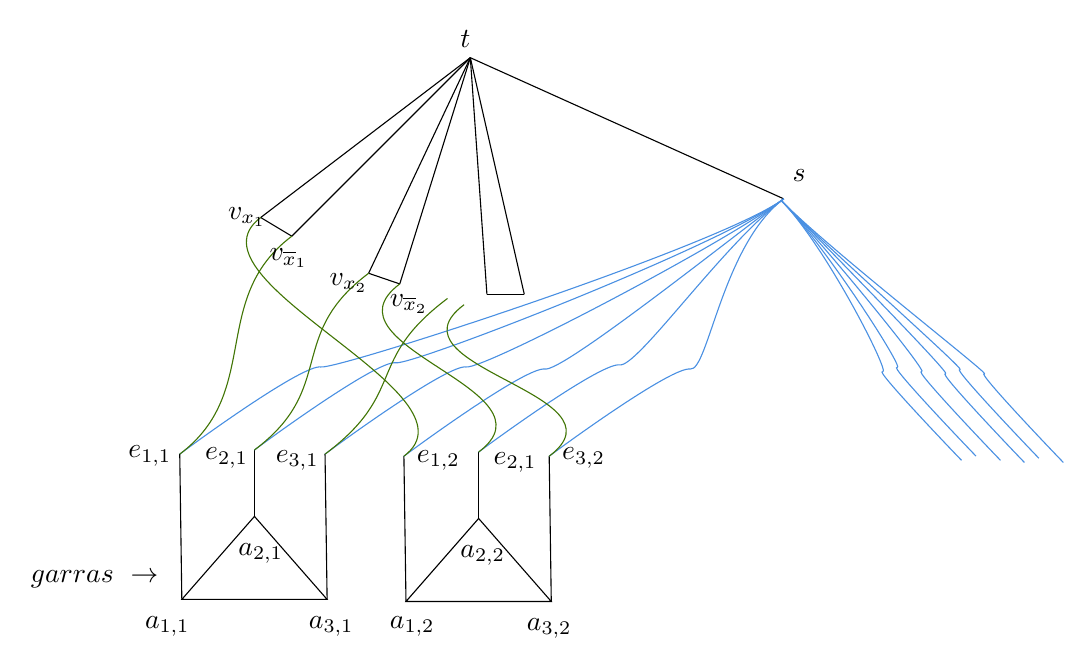
\begin{tikzpicture}[x=0.75pt,y=0.75pt,yscale=-1,xscale=1]
    %uncomment if require: \path (0,345); %set diagram left start at 0, and has height of 345

    %Straight Lines [id:da024577145388274158] 
    \draw    (282,24) -- (181,101) ;
    %Straight Lines [id:da9147970884158108] 
    \draw    (282,24) -- (196,110) ;
    %Straight Lines [id:da24241664675971752] 
    \draw    (282,24) -- (233,127.86) ;
    %Straight Lines [id:da0019185310537932487] 
    \draw    (282,24) -- (248,133) ;
    %Straight Lines [id:da7044595354738321] 
    \draw    (282,24) -- (290,138) ;
    %Straight Lines [id:da12066461117319749] 
    \draw    (282,24) -- (308,138) ;
    %Straight Lines [id:da9216806050314463] 
    \draw    (282,24) -- (433,92) ;
    %Straight Lines [id:da8579836464252726] 
    \draw    (181,101) -- (196,110) ;
    %Straight Lines [id:da33046636333965984] 
    \draw    (233,127.86) -- (248,133) ;
    %Straight Lines [id:da8169841491168588] 
    \draw    (290,138) -- (308,138) ;
    %Shape: Triangle [id:dp5066112718925191] 
    \draw   (178,245) -- (213,285) -- (143,285) -- cycle ;
    %Straight Lines [id:da987499546806103] 
    \draw    (178,213) -- (178,245) ;
    %Straight Lines [id:da2327644054665976] 
    \draw    (212,215) -- (213,285) ;
    %Straight Lines [id:da6985649002842926] 
    \draw    (142,215) -- (143,285) ;
    %Shape: Triangle [id:dp9994407735338462] 
    \draw   (286,246) -- (321,286) -- (251,286) -- cycle ;
    %Straight Lines [id:da9924493799376253] 
    \draw    (286,214) -- (286,246) ;
    %Straight Lines [id:da27535775663210726] 
    \draw    (320,216) -- (321,286) ;
    %Straight Lines [id:da2242309455971152] 
    \draw    (250,216) -- (251,286) ;
    %Curve Lines [id:da11992808862863669] 
    \draw [color={rgb, 255:red, 74; green, 144; blue, 226 }  ,draw opacity=1 ]   (142,215) .. controls (152.54,207.09) and (201.5,171.7) .. (210,173) .. controls (218.5,174.3) and (403.54,114.09) .. (433,92) ;
    %Curve Lines [id:da7810373386432186] 
    \draw [color={rgb, 255:red, 74; green, 144; blue, 226 }  ,draw opacity=1 ]   (178,213) .. controls (188.54,205.09) and (237.5,169.7) .. (246,171) .. controls (254.5,172.3) and (403.54,114.09) .. (433,92) ;
    %Curve Lines [id:da7610424465229726] 
    \draw [color={rgb, 255:red, 74; green, 144; blue, 226 }  ,draw opacity=1 ]   (212,215) .. controls (222.54,207.09) and (271.5,171.7) .. (280,173) .. controls (288.5,174.3) and (403.54,114.09) .. (433,92) ;
    %Curve Lines [id:da4850711005271304] 
    \draw [color={rgb, 255:red, 74; green, 144; blue, 226 }  ,draw opacity=1 ]   (250,216) .. controls (260.54,208.09) and (309.5,172.7) .. (318,174) .. controls (326.5,175.3) and (403.54,114.09) .. (433,92) ;
    %Curve Lines [id:da8453334931293217] 
    \draw [color={rgb, 255:red, 74; green, 144; blue, 226 }  ,draw opacity=1 ]   (286,214) .. controls (296.54,206.09) and (345.5,170.7) .. (354,172) .. controls (362.5,173.3) and (403.54,114.09) .. (433,92) ;
    %Curve Lines [id:da5079195764877538] 
    \draw [color={rgb, 255:red, 74; green, 144; blue, 226 }  ,draw opacity=1 ]   (320,216) .. controls (330.54,208.09) and (379.5,172.7) .. (388,174) .. controls (396.5,175.3) and (403.54,114.09) .. (433,92) ;
    %Curve Lines [id:da8271646687449208] 
    \draw [color={rgb, 255:red, 74; green, 144; blue, 226 }  ,draw opacity=1 ]   (518.66,217.98) .. controls (510.9,209.95) and (476.64,173.98) .. (480.66,175.31) .. controls (484.68,176.63) and (453.68,115.45) .. (432,93) ;
    %Curve Lines [id:da6033929929298949] 
    \draw [color={rgb, 255:red, 74; green, 144; blue, 226 }  ,draw opacity=1 ]   (525.63,215.95) .. controls (517.87,207.92) and (483.61,171.95) .. (487.63,173.27) .. controls (491.65,174.6) and (453.68,115.45) .. (432,93) ;
    %Curve Lines [id:da7047394504171489] 
    \draw [color={rgb, 255:red, 74; green, 144; blue, 226 }  ,draw opacity=1 ]   (537.42,217.98) .. controls (529.66,209.95) and (495.41,173.98) .. (499.43,175.31) .. controls (503.45,176.63) and (453.68,115.45) .. (432,93) ;
    %Curve Lines [id:da6505082289688271] 
    \draw [color={rgb, 255:red, 74; green, 144; blue, 226 }  ,draw opacity=1 ]   (548.95,219) .. controls (541.19,210.97) and (506.93,175) .. (510.95,176.32) .. controls (514.97,177.65) and (453.68,115.45) .. (432,93) ;
    %Curve Lines [id:da3291128010874702] 
    \draw [color={rgb, 255:red, 74; green, 144; blue, 226 }  ,draw opacity=1 ]   (555.92,216.97) .. controls (548.16,208.93) and (513.9,172.97) .. (517.92,174.29) .. controls (521.94,175.61) and (453.68,115.45) .. (432,93) ;
    %Curve Lines [id:da1520010028888894] 
    \draw [color={rgb, 255:red, 74; green, 144; blue, 226 }  ,draw opacity=1 ]   (567.71,219) .. controls (559.95,210.97) and (525.69,175) .. (529.71,176.32) .. controls (533.73,177.65) and (453.68,115.45) .. (432,93) ;
    %Curve Lines [id:da7481436423375991] 
    \draw [color={rgb, 255:red, 65; green, 117; blue, 5 }  ,draw opacity=1 ]   (142,215) .. controls (182,185) and (156,140) .. (196,110) ;
    %Curve Lines [id:da00851059064414783] 
    \draw [color={rgb, 255:red, 65; green, 117; blue, 5 }  ,draw opacity=1 ]   (178,213) .. controls (218,183) and (193,157.86) .. (233,127.86) ;
    %Curve Lines [id:da7905929568459347] 
    \draw [color={rgb, 255:red, 65; green, 117; blue, 5 }  ,draw opacity=1 ]   (212,215) .. controls (252,185) and (231,170) .. (271,140) ;
    %Curve Lines [id:da5572121126151761] 
    \draw [color={rgb, 255:red, 65; green, 117; blue, 5 }  ,draw opacity=1 ]   (250,216) .. controls (290,186) and (141,131) .. (181,101) ;
    %Curve Lines [id:da9639491981576338] 
    \draw [color={rgb, 255:red, 65; green, 117; blue, 5 }  ,draw opacity=1 ]   (286,214) .. controls (326,184) and (208,163) .. (248,133) ;
    %Curve Lines [id:da32366690739652726] 
    \draw [color={rgb, 255:red, 65; green, 117; blue, 5 }  ,draw opacity=1 ]   (320,216) .. controls (360,186) and (239,173) .. (279,143) ;

    % Text Node
    \draw (436,76.8) node [anchor=north west][inner sep=0.75pt]    {$s$};
    % Text Node
    \draw (276,9.8) node [anchor=north west][inner sep=0.75pt]    {$t$};
    % Text Node
    \draw (164,94.8) node [anchor=north west][inner sep=0.75pt]    {$v_{x_{1}}$};
    % Text Node
    \draw (213,126.8) node [anchor=north west][inner sep=0.75pt]    {$v_{x_{2}}$};
    % Text Node
    \draw (184,114.8) node [anchor=north west][inner sep=0.75pt]    {$v_{\overline{x}_{1}}$};
    % Text Node
    \draw (242,136.8) node [anchor=north west][inner sep=0.75pt]    {$v_{\overline{x}_{2}}$};
    % Text Node
    \draw (265,123.8) node [anchor=north west][inner sep=0.75pt]    {$\dotsc $};
    % Text Node
    \draw (124,291.8) node [anchor=north west][inner sep=0.75pt]    {$a_{1,1}$};
    % Text Node
    \draw (203,291.8) node [anchor=north west][inner sep=0.75pt]    {$a_{3,1}$};
    % Text Node
    \draw (169,256.8) node [anchor=north west][inner sep=0.75pt]    {$a_{2,1}$};
    % Text Node
    \draw (242,291.8) node [anchor=north west][inner sep=0.75pt]    {$a_{1,2}$};
    % Text Node
    \draw (308,292.8) node [anchor=north west][inner sep=0.75pt]    {$a_{3,2}$};
    % Text Node
    \draw (276,257.8) node [anchor=north west][inner sep=0.75pt]    {$a_{2,2}$};
    % Text Node
    \draw (116,209.8) node [anchor=north west][inner sep=0.75pt]    {$e_{1,1}$};
    % Text Node
    \draw (153,210.8) node [anchor=north west][inner sep=0.75pt]    {$e_{2,1}$};
    % Text Node
    \draw (187,211.8) node [anchor=north west][inner sep=0.75pt]    {$e_{3,1}$};
    % Text Node
    \draw (255,211.8) node [anchor=north west][inner sep=0.75pt]    {$e_{1,2}$};
    % Text Node
    \draw (292,212.8) node [anchor=north west][inner sep=0.75pt]    {$e_{2,1}$};
    % Text Node
    \draw (325,210.8) node [anchor=north west][inner sep=0.75pt]    {$e_{3,2}$};
    % Text Node
    \draw (378,247.8) node [anchor=north west][inner sep=0.75pt]    {$\dotsc $};
    % Text Node
    \draw (69,269.8) node [anchor=north west][inner sep=0.75pt]    {$garras\ \rightarrow $};
    \end{tikzpicture}
\end{figure}

Observemos que $G$ tiene un triangulo, por lo que
$$\chi(G) \< 3 \Leftrightarrow \chi(G) = 3$$

Probemos primero:
$$\chi(G) = 3 \Rightarrow B \text{ es satisfacible}$$

Como $\chi (G) = 3$ entonces existe un locoreo propio de $G$ con $3$ colores, 
llamemosle $C$.
\medskip

Necesitamos definir un vector $(b_{1},b_{2},\ldots ,b_{n}) \in \llaves{0,1}^{n}$ 
tal que $B(\overrightarrow{b}) = 1$.
\medskip

Entonces, en base al coloreo $C$ definimos:
$$b_{i}= \left\{ \begin{array}{lcc}
    1 & \to & C(v_{x_{i}} = C(s) \\
    \\ 0& \to & c.c\\
    \end{array}
    \right.$$

Queremos ver $B(\overrightarrow{b}) = 1$ basta ver que $D_{j}(\overrightarrow{b}) = 1\,\, \forall j$. 
Entonces tomemos un $j$ cualquiera, como para todo $j$ los $a_{1,j}a_{2,j}a_{3,j}$ 
forman un triangulo entonces los $3$ colores deben aparece ahí.
\medskip

En particular $\exists i: C(a_{i,j}) = C(t)$ (voy desde la garra hacia arriba). 
\medskip

Como $e_{i,j}a_{i,j} \in E \Rightarrow C(e_{i,j}) \neq C(t)$.
\medskip

Como $e_{i,j}s \in E \Rightarrow C(e_{i,j}) \neq C(s)$.
\medskip

Como $ts \in E \Rightarrow C(t) \neq C(s)$.
\medskip

Entonces $C(e_{i,j}) = \text{tercer color}$ (el color que es distinto del color de 
$s$ y $t$).
\medskip

Ahora ya sabemos que color tienen los extremos de las garras. Entonces, vemos que
$v_{l_{i},j}e_{i,j} \in E \Rightarrow C(v_{l_{i},j}) \neq C(e_{i,j}) = \text{tercer color}$.
$\Rightarrow C(v_{l_{i},j}) = C(t)$ o $C(s)$
\medskip

Pero $tv_{l_{i},j} \in E \Rightarrow C(v_{l_{i},j})\neq C(t)$ entonces no queda 
otra que $C(v_{l_{i},j}) = C(s)$ que es el candidato para cuando evalue en $b_{i}=1$.
\medskip

El $l_{i,j}$ es un literal por lo tanto es una variable o una negación. Veamos 
primero el caso que es una variable:
\medskip

Entonces $\exists k : l_{i,j} = x_{k}$ entonces $v_{l_{i},j} = v_{x_{k}}$ a su vez 
se da que $C(v_{l_{i},j}) = C(s) \Rightarrow C(v_{x_{k}}) = C(s) \Rightarrow b_{k} = 1$.
\medskip

Entonces $l_{i,j} = x_{k} \Rightarrow l_{i,j}(\overrightarrow{b}) = x_{k}(\overrightarrow{b}) = b_{k} = 1 \Rightarrow D_{j}(\overrightarrow{b}) = 1$.
\medskip

Supongamos ahora que es negación de una variable:
$\exists k: l_{i,j} = \bar{x}_{k} \Rightarrow l_{i,j}(\overrightarrow{b}) = \bar{x}_{k}(\overrightarrow{b}) = 1 + b_{k}$

Por $k: l_{i,j} = \bar{x}_{k}$ podemos decir que $C(s) = C(v_{l_{i},j}) = C(v_{\bar{x}_{k}})$
\medskip

Pero $v_{x_{k}}v_{\bar{x}_{k}} \in E \Rightarrow C(v_{x_{k}}) \neq C(v_{\bar{x}_{k}})$
\medskip

Como son distintos y $C(v_{\bar{x}_{k}}) = C(s)$ entonces $C(v_{x_{k}}) \neq C(s) \Rightarrow b_{k} = 0$
\medskip

Entonces $\bar{x}_{b}(\overrightarrow{b}) = 1+0 = 1$

$(\Leftarrow)$ 

$$B \text{ es satisfacible} \Rightarrow \chi(G) \< 3$$

Supongamos $B$ satisfacible $\Rightarrow \exists \overrightarrow{b} \in \llaves{0,1}^{n} : B(\overrightarrow{b}) = 1$ 
y hay que definir un coloreo a partir de esto. Entonces, debemos definir un coloreo 
$C$.
\medskip

Definimos $C(s) = 1$ y $C(t) =2$. Hay que analizar si el coloreo es propio en cada caso.
\medskip

Entonces el lado $st$ no crea problemas $(NCP)$.
\medskip

Para los $v_{l}$ definimos, $C(v_{l}) = l(\overrightarrow{b})$, en otras palabras:
\begin{align*}
    C(v_{x_{i}}) &= b_{i} \in (0,1) \\
    C(v_{\bar{x}_{i}}) &= 1 + b_{i} \in (0,1)
\end{align*}

Entonces hay que ver los casos:
$$\underbrace{v_{x_{i}}}_{0\,\,\text{ó}\,\,1} \underbrace{v_{\bar{x}_{i}}}_{1\,\,\text{ó}\,\,0} \Rightarrow NCP $$

$$\underbrace{v_{l}}_{0\,\,\text{ó}\,\,1} \underbrace{t}_{2} \Rightarrow NCP $$

Ahora como $B(\overrightarrow{b}) = 1$ (esto hay que usarlo si o si) entonces 
$D_{j}(\overrightarrow{b}) = 1\,\, \forall j$.
\medskip

$$\Rightarrow \forall j \exists i = i_{j} : l_{i_{j},j}(\overrightarrow{b}) = 1$$

Si hay más de uno elijo uno por ejemplo el primero.
\medskip

Coloreamos los $a_{i,j}$ de la siguiente forma (base de la garra)
\begin{align*}
    C(a_{i_{j},j}) &= 2 \\
    C(a_{i,j})_{con\,\, i = i_{j}} &= \text{le doy color $1$ a uno y $0$ al otro}
\end{align*}

Cómo los colores de las $a_{i,j}$ son $0,1,2$ entonces el triangulo $NCP$ y coloreamos 
los $e's$ de la siguiente forma:
$$C(e_{i,j})= \left\{ \begin{array}{lcc}
    2 & \to & i \neq i_{j} \\
    \\ 0& \to & i = i_{j}\\
    \end{array}
    \right.$$

Chequeamos los lados:
\begin{align*}
    &i \neq i_{j} \to \underbrace{a_{i,j}}_{0\,\,\text{ó}\,\,1}\underbrace{e_{i,j}}_{2} \Rightarrow NCP \\
    &i = j \to \underbrace{a_{i_{j},j}}_{2}\underbrace{e_{i_{j},j}}_{0} \Rightarrow NCP \\
    &\underbrace{s}_{1}\underbrace{e_{i,j}}_{0\,\,\text{ó}\,\,2} \Rightarrow NCP \\
    &\text{solo queda ver los}\,\, e_{i,j}v_{l_{i},j}\\
    &i \neq i_{j} \to \underbrace{e_{i,j}}_{2}\underbrace{v_{l_{i},j}}_{0\,\,\text{ó}\,\,1} \Rightarrow NCP \\
    &i = i_{j} \to \\
    &C(e_{i_{j},j}) = 0\\
    &C(v_{v_{l_{i_{j},j}}}) = l_{i_{j},j}(\overrightarrow{b}) = 1\\
    &\text{es igual a $1$ por la elección del $i_{j}$}\\
    &\Rightarrow \underbrace{e_{i,j}}_{0}\underbrace{v_{l_{i},j}}_{1} \Rightarrow NCP
\end{align*}
$\square$

\end{document}